\documentclass[a4paper, twoside, 12pt]{book}

\usepackage[french]{babel}
%--------------------------
% INPUTENC (encodage du texte)
% FONTENC (positionnement des accents)
%--------------------------
%\usepackage[utf8]{inputenc}
%\usepackage{ae,lmodern}
\usepackage[T1]{fontenc}
% Interligne
\usepackage{setspace}

%Pour gérer caractères spéciaux °
%\DeclareUnicodeCharacter{00B0}{ }
%Pour les épigraphes
\usepackage{epigraph}
\setlength{\epigraphrule}{0pt}
\setlength{\epigraphwidth}{0.6\textwidth}
 \renewcommand\textflush{flushepinormal}
 \renewenvironment{flushepinormal}{}{\vspace*{-\baselineskip}}
\usepackage{booktabs} % Required for better table rules
% Title page details: 
%--------------------------
% HYPERREF (liens hypertextes et métadonnées)
%--------------------------
\usepackage{hyperref}
\hypersetup{%
colorlinks=true,
linkcolor=black,
urlcolor=blue,
citecolor=black
}

%--------------------------
% TOCBIBIND (ajouter la bibliographie dans la Table des matières)
%--------------------------
%\usepackage{tocbibind}
\usepackage[nottoc,notlot,notlof]{tocbibind}
%--------------------------
% Éléments de mise en page (marge de 2,5 cm, alinéa en début de paragraphe 1cm, interligne 1,5)
%--------------------------
\usepackage[a4paper, margin=2.5cm]{geometry}
\usepackage{setspace}
\onehalfspacing
\setlength{\parindent}{1cm}

\usepackage{fancyhdr}
\setlength{\headheight}{28pt}
\renewcommand{\chaptermark}[1]{\markboth{#1}{}}
\renewcommand{\sectionmark}[1]{\markright{#1}}
\pagestyle{fancy}
\fancyhf{}
\fancyhead[LE,RO]{\thepage}
\fancyhead[LO]{\nouppercase{\rightmark}}
\fancyhead[RE]{\nouppercase{\leftmark}}
\renewcommand{\headrulewidth}{0pt}

%--------------------------
% Modules pour gérer les listes
%--------------------------
\usepackage{enumerate}
\usepackage{enumitem}


%--------------------------
% BIBLIOGRAPHIE
%--------------------------
\usepackage[backend=biber, sorting=nyt, style=enc]{biblatex}
\usepackage[autostyle]{csquotes}

\addbibresource{biblio/Genre & style.bib}
\addbibresource{biblio/Humanités numériques.bib}
\addbibresource{biblio/Le Pamphlet.bib}
\addbibresource{biblio/Sources.bib}

\setcounter{secnumdepth}{5}
\setcounter{tocdepth}{2}

\usepackage[official]{eurosym}
\usepackage{afterpage}
\usepackage{booktabs,xltabular}
%--------------------------
% FIGURES
%--------------------------
\usepackage{graphicx}
\graphicspath{ {./images/} }
\usepackage{float}
\usepackage{multirow}
\usepackage{longtable}


\usepackage{enumerate,lettrine}
\usepackage{tipa}


\title{Mémoire M2 HN ENC-PSL }
\author{Louis-Fiacre Franchet d'Espèrey}

%----------------------------------------------------------------------------------------
\begin{document}

\frontmatter

\begin{titlepage}
\begin{center}

\bigskip

\begin{large}
UNIVERSITÉ PARIS, SCIENCES \& LETTRES
\end{large}
%TODO: nom établissement de préparation
\begin{center}\rule{2cm}{0.02cm}\end{center}

\bigskip
\bigskip
\bigskip
\begin{Large}
\textbf{Louis-Fiacre Franchet d'Espèrey}\\
\end{Large}
\begin{normalsize} \textit{licencié ès lettres}\\
\textit{licencié d'histoire}\\
\end{normalsize}

\bigskip
\bigskip
\bigskip

\begin{Huge}
\textbf{Le pamphlet, un genre littéraire ?}\\
\end{Huge}
\bigskip
\bigskip
\begin{LARGE}
\textbf{Étude textométrique du genre pamphlétaire}\\
\end{LARGE}

\bigskip
\bigskip
\bigskip
\begin{large}
\end{large}
\vfill

\begin{large}
Mémoire 
pour le diplôme de master \\
\og Humanités numériques et computationnelles \fg{} \\
\bigskip
2021 - 2023
\end{large}

\end{center}
\end{titlepage}

\thispagestyle{empty}
\cleardoublepage

\section*{Résumé}
\addcontentsline{toc}{chapter}{Résumé}

Cette étude propose d'étudier le pamphlet en tant que genre littéraire. Le pamphlet est un phénomène littéraire propre au XIXe siècle qui a connu une grande popularité jusqu'à la seconde guerre mondiale et qui tend depuis à se résorber voire à disparaître. Une étude générique de l'écriture pamphlétaire combinant des méthodes issues des sciences computationnelles avec des analyses stylistiques permettra d'étoffer le champ de recherche des marges de la littérature d'où ce genre est relégué. Le pamphlet comme phénomène politique et historique circonstancié a pu être étudié au travers de nombreux axes de recherche autre que littéraire. Après les travaux de Marc Angenot sur la typologie du pamphlet \textit{La Parole pamphlétaire, Contribution a la typologie des discours modernes, Payot, 1982}, nous considérons que l'apport de méthodes computationnelles pourront enrichir le regard de la recherche sur le objet littéraire qu'est le pamphlet. Nous mobiliserons pour cette étude des outils de textométrie, de linguistique et de stylistique pour analyser la spécificité de l'écriture pamphlétaire.

\medskip

\textbf{Mots-clés:} Genre; Pamphlet; Stylistique; Humanités numériques; Textométrie

\textbf{Informations bibliographiques:} Louis-Fiacre Franchet d'Espèrey, \textit{Le pamphlet, un genre littéraire ?: Étude textométrique du genre pamphlétaire}, mémoire de master 2 \og Humanités numériques et computationnelles\fg{}, dirs. Camps, Jean-Baptiste et PAILLET Anne-Marie, Université Paris, Sciences \& Lettres, 2023.

\section*{Abstract}
\addcontentsline{toc}{chapter}{Abstract}
This study undertakes an examination of the pamphlet as a literary genre. The pamphlet emerged as a distinctive literary phenomenon during the 19th century, achieving considerable popularity until the outbreak of the Second World War, subsequently undergoing a process of obsolescence. Employing a synthetic approach informed by both computational methodologies and stylistic analyses, this investigation aims to expand the scholarly purview into the peripheries of the literary domain to which the pamphlet has been relegated. In addition to its conventional literary considerations, the pamphlet, as a nuanced political and historically contingent phenomenon, has been subject to multivarious investigatory trajectories. Building upon the foundational typological framework established by Marc Angenot \textit{La Parole pamphlétaire, Contribution a la typologie des discours modernes, Payot, 1982}, we posit that the incorporation of computational methodologies stands to augment the scholarly inquiry into the distinct literary object that is the pamphlet. Leveraging tools encompassing textometric analysis, linguistic examination, we will engage in a comprehensive exploration of the distinctive qualities underpinning pamphlet composition.
\medskip

\textbf{Keywords:} Genre; Pamphlet; Stylistics; Digital Humanities; Textometry

\textbf{Bibliographic Information:} Louis-Fiacre Franchet d'Espèrey, \textit{Le pamphlet, un genre littéraire ?: Étude textométrique du genre pamphlétaire}, M.A. thesis \og Digital and computational humanities\fg{}, dirs. Camps, Jean-Baptiste et PAILLET Anne-Marie, Université Paris, Sciences \& Lettres, 2023.

\clearpage
\thispagestyle{empty}
\cleardoublepage

\chapter*{Remerciements}
\addcontentsline{toc}{chapter}{Remerciements}
\bigskip
\lettrine{M}{es remerciements} vont tout d'abord à mes directeurs de recherche: Monsieur Jean-Baptiste Camps pour sa pédagogie, et ses conseils avisés et Madame Anne-Marie Paillet pour sa patience et son plaisir de transmettre que se soit dans ses séminaires de stylistique comme dans son atelier de diction et de théâtre. \\
Je veux aussi remercier Monsieur Chahan Vidal-Gorène pour ses nombreux conseils ainsi que pour sa grande disponibilité.\\
Je tiens aussi à remercier Cédric Passard pour le temps qu'il a pu consacrer à me relire.\\
Mais aussi je souhaite adresser ma gratitude à la promotion des masterants HN des chartes 2023 qui fut dans chacun de ses membres pendant deux belles années une source d'inspiration merveilleuse.\\
Mes remerciements sont aussi adressés à ma tendre épouse qui fut durant ce temps béni des études, une aide et un soutien précieux.

\clearpage
\thispagestyle{empty}
\cleardoublepage

\addcontentsline{toc}{chapter}{Bibliographie}
\nocite{*}
\printbibliography[keyword={Genre \& style}, title={Linguistique et stylistique}]
\printbibliography[keyword={pamphlet}, title={Genre du pamphlet}]
\printbibliography[keyword={HN}, title={Humanités numériques}]
\printbibliography[keyword={sources}, title={Sources}]
\clearpage


\mainmatter

\part*{Introduction}
\addcontentsline{toc}{part}{Introduction}
\markboth{Introduction}{Introduction}

\vspace*{\fill}
\epigraph{\enquote{  Pamphlétaire !\ldots  Ah ! je suis autre chose, pourtant… mais si je suis pamphlétaire, moi, je le suis par indignation et par amour ; et mes cris, je les pousse, dans mon désespoir morne, sur mon Idéal saccagé !\ldots  }}{\textit{Léon Bloy, Le Bon Conseil, Belluaires et porchers Paris, 28 mai 1892. }}

\vfill\clearpage
\chapter{Préliminaires}
Cette étude se propose d'analyser le genre du pamphlet avec des méthodes stylistiques et textométriques. Un des objectifs de ce travail est de tirer parti des méthodes computationnelles pour vérifier à une plus grande échelle certaines hypothèses sur les spécificités du genre pamphlétaire issues d'analyses stylistiques. Le pamphlet comme sujet de recherche fut longtemps déconsidéré, étant situé en marge de la littérature dite classique. Le pamphlet, par sa violence extrême, ses sujets de controverses d'une actualité dépassée ou son parfum de scandale, n'était pas voué à conserver une valeur littéraire quelconque, ce qui peut expliquer un certain désintérêt pour son étude. Il y eu un regain d'intérêt pour ce champ d'étude avec le travail de Marc Angenot sur la typologie pamphlétaire \footcites{angenot_parole_1982} dont notre propos se voudra être un prolongement par le déploiement de méthodes computationnelles. Ce travail s'appuiera notamment sur les domaines de la qualification et de la classification des genres à l'aune des humanités numériques.

Au tournant du XIX\ieme siècle, une forme nouvelle de littérature est apparue. Elle a considérablement marqué la vie politique française, a révélé ou fantasmé des scandales d'état, a détruit des réputations, a engendré des monuments littéraires pour finalement péricliter dans la seconde moitié du XX\ieme siècle jusqu'à quasiment disparaître de nos jours. Cette littérature nouvelle fut le pamphlet. Phénomène littéraire, ambigu et protéiforme, le pamphlet connu son âge d'or de 1868 à 1968 et fut un marqueur fort de la fin du XIX\ieme 
 siècle agité de la vie littéraire et médiatique française.

L'analyse du discours moderne en littérature s'est considérablement développée sur l'étude des formes canoniques de la fiction et de la poétique; la littérature de combat dont le pamphlet fait partie, peut sembler être le parent pauvre de cette recherche. La nature même du pamphlet comme écrit de circonstance (dont la littérarité passe souvent au second plan d'une volonté persuasive) se démarque fortement des formes classiques de la littérature (des écrits pour durer dont la littérarité est au premier plan). Une difficulté supplémentaire s'ajoutant, pour étudier le phénomène pamphlétaire, est que ce champ d'étude n'est pas clairement circonscris et ce pour plusieurs raisons : le qualificatif de pamphlet est utilisé par une multitude d'acteurs différents et parfois récusé par les auteurs eux-mêmes. Aussi les distinctions de la forme du pamphlet, face à d'autres modèles plus anciens, tel que la \textit{diatribe}, \textit{l'opuscule}, la \textit{brochure}, le \textit{brûlot} et de nombreux autres encore, ne sont pas d'une évidence formelle. Nous proposons dans cette présente étude d'ouvrir des pistes de recherche de définition du genre pamphlétaire en utilisant des méthodes quantitatives en soutien à une analyse stylistique. Cette étude part du présupposé que le style propre d'écrivains se combine aux exigences du genre littéraire dans lequel il écrit, et que ces inclinaisons à écrire dans un genre donné et d'une certaine manière, peut correspondre à définir certains aspects spécifiques de ce genre.

\chapter{Historiographie du pamphlet}

Une longue tradition de texte polémique et satirique existe en France bien avant la Révolution française et l'apparition du pamphlet, on peut citer les \textit{mazarinades}, les \textit{pasquinades}, les \textit{libelles}, \textit{diatribes}, les \textit{placards}, \textit{brulôts} et bien d'autres dont le pamphlet se retrouve en être une forme héritière, nouvelle et concurrente.
Le pamphlet est un phénomène littéraire circonscris dans une période historique, le XIX\ieme siècle français. Avec les différentes lois régissant la liberté de la presse, et la massification des publications, ce siècle fut propice au développement d'une littérature polémique considérablement plus violente que sous l'ancien régime. Les conditions de développement historique du pamphlet furent étudiés par Cédric Passard dans \textit{L'Âge d'or du pamphlet}\footcites{passard_lage_2015}. De nombreux facteurs techniques, politiques et moraux permettent, non pas d'expliquer, mais de se renseigner sur le développement fulgurant des pratiques politiques et culturelles nouvelles de \textit{l'écrit de combat}.

L'usage du mot pamphlet est une nouveauté pour le XIX\ieme siècle français, de nombreuses autres formes synonymes avaient cours sous l'ancien régime. Sans forcément supplanter ces mots (le terme brochure resta concurrent mais bien plus général durant l'ensemble du XIX\ieme siècle) le terme pamphlet permis de définir un type spécifique divergeant des précédents synonymes évoqués et des modèles plus anciens de la satire et de la polémique. 

\begin{figure}[H]
\centering %
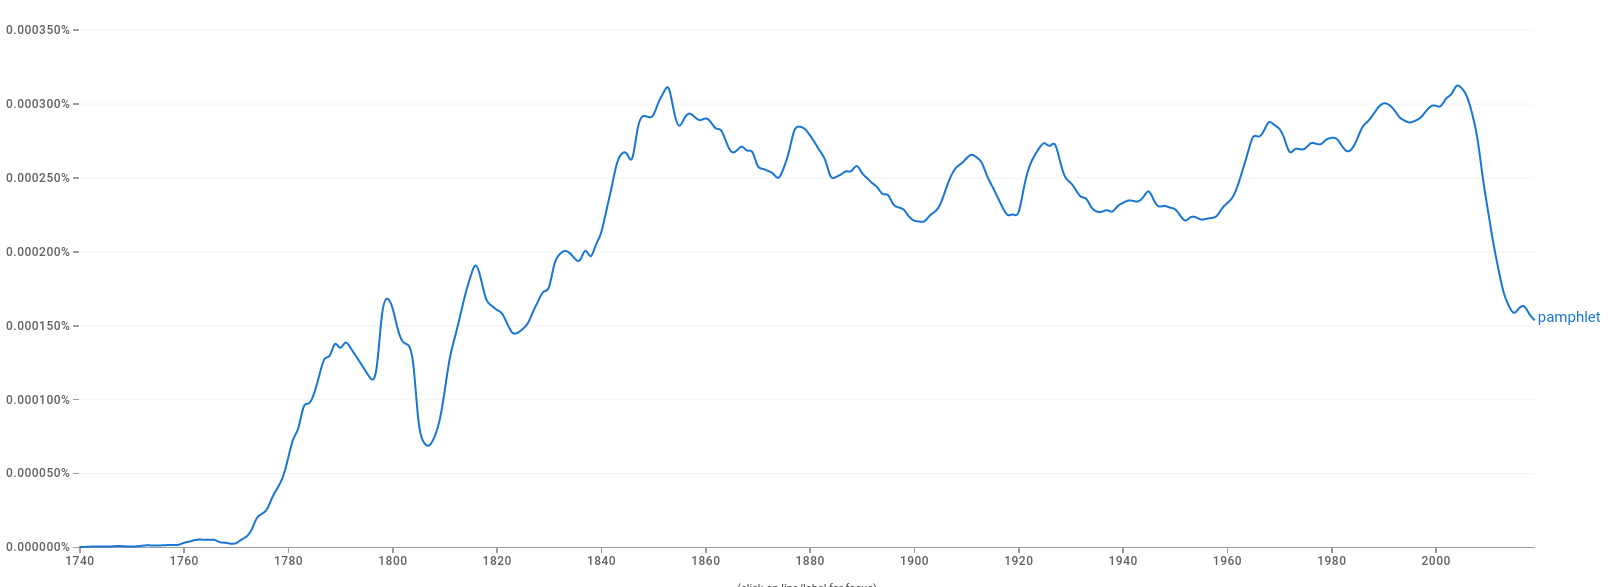
\includegraphics[width=1\textwidth]{img/google_ngramviewer_pamphlet_french_2019.png}
\caption{\textit{Visualisation de la fréquence d'emploi du terme pamphlet de 1740 à 2019, Google ngram Viewer, french corpus 2019}}
\label{fig:googlengram}
\end{figure}

La figure \textit{\ref{fig:googlengram}} montre l'ascension spectaculaire du terme \textit{pamphlet} de la fin du XVIII\ieme au début du XIX\ieme siècle. Il est intéressant de noter que certaines baisses de fréquence du mot ont l'air d'être directement corrélés aux périodes politiques propices à des lois encadrant strictement la presse. Sur la figure nous constatons trois pics baissiers qui peuvent correspondre aux période de la Terreur, de la Terreur blanche (sous la 1\iere Restauration avec la loi du 9 novembre 1815 sur les cris et écrits sédicieux \footcites{quensoi_de_la_hennerie_les_1925} qui fut adouci par la loi du 17 mai 1819) et de la seconde Restauration jusqu'aux ordonnances de juillet (dont la première ordonnance restreignait encore plus les libertés de la presse) et la révolution des Trois Glorieuses.

Sur la polysémie du mot pamphlet, le \textit{Dictionnaire de l'Académie française} donne à ce propos la définition suivante du terme pamphlet de la 4\ieme  édition de 1762 jusqu'à la 6\ieme  édition de 1835 : \enquote{\textit{Mot Anglois, qui s'emploie quelquefois dans notre langue, et qui signifie Brochure.}}\footcites{francaise_dictionnaire_nodate}. À l'entrée \textit{Brochure} de la 2\ieme  édition : \enquote{\textit{Petit ouvrage de peu de feüilles, qui n'est pas relié comme un Livre ; mais qui est seulement broché}}. Cette association du mot pamphlet à celui de brochure est présente jusqu'à la 8\ieme édition de 1935. Nous voyons que le rapport des deux termes est établi par la similitude de l'objet papier et non par son contenu bien qu'une grande partie des brochures ait pu traiter de politique. Paul-Louis Courrier relate dans \textit{le Pamphlet des pamphlets} son procès perdu à cause de l'ambiguïté du terme pamphlet entre écrit court et écrit injurieux, les contemporains du XIX\ieme siècle employaient le terme de pamphlet pour un grand nombre de texte divers et pour des raisons toutes aussi diverses et hétérogènes. 

\section{Une étymologie d'origine médiévale}

L'origine du terme à longtemps été controversée. Le \textit{Trésor de la Langue Française informatisé}\footcites{noauthor_tlfi_nodate} (TLFi) fait remonter la première occurrence du terme de pamphlet à Henri D'Andeli dans son poème la \textit{Bataille des VII Arts} de la moitié du XIII\ieme siècle, \textit{\enquote{La fu li sage Chatonez, Avionès et Panfilès}}.\footcites{henri_dandeli_oeuvres_1881} La forme \textit{Panfilès} est issue de Pamphile, suivant une évolution linguistique par nominalisation d'un nom propre par antonomase. Il existe plusieurs exemples de ce processus en Ancien Français, comme le recueil de fables attribué à Ésope se nomme \textit{\enquote{Isopet}} ou \textit{\enquote{Esopet}} comme l'\textit{\enquote{Avionès}} ou \textit{\enquote{Avionet}} est un poème d'Avianus et le \textit{\enquote{Chatonez}} ou \textit{\enquote{Catonet}} est un poème de Caton\footcites{morawski_pamphile_1917}. Ainsi le \textit{\enquote{Panfilès}} ou \textit{\enquote{pamphilet}} est le résultat d'une antonomase de Pamphile, désignant un ouvrage. \textit{le Pamphilus de amore}, \textit{Pamphile ou l'art d'être aimer} est une comédie latine très courte de 780 vers datant du X\ieme siècle, dont l'origine oscille entre la France et l'Espagne. Nous ne nous attarderons pas sur ce poème mais simplement, le sujet est d'une ironie assez marquée car le protagoniste éponyme, par le viol de Galatée, l'objet de son désir amoureux, échoue en amour. Cette comédie eu une grande influence dans toute l'Europe et on en retrouve une belle part dans l'inspiration du \textit{Roman de la Rose} et chez Geoffrey Chaucer, grand littérateur anglais du XIV\ieme siècle\footcites{morawski_pamphile_1917}. Le lien entre cette comédie et le genre du pamphlet se profile par deux prédicats communs, l'usage de l'ironie et la concision de l'ouvrage. La dimension européenne de la diffusion de cette comédie donne lieu, en 1344, au terme \textit{panfletus} du latin médiéval d'Angleterre qui se transforme en 1387-8 en \textit{pampflet} : \enquote{\textit{désignant parfois plus particulièrement une brochure sur un sujet d'actualité, éventuellement de politique ou propre à la controverse}} toujours d'après le TLFi. Les brochures, comme les opuscules sont de petits livrets qui circulaient par des canaux de diffusion non contrôlés par les instances politiques. La rapidité d'impression d'un ouvrage est associable à sa circulation clandestine, d'où la part importante de pamphilet à dimension ironique, satirique ou polémique. Cela préfigure notre acception moderne du pamphlet comme un texte utilisant les registres de l'ironie et de la polémique et de peu de pages.

\section{Libelle et pamphlet à l'époque moderne}
Le mot apparaît en français pour la première fois en 1653 dans \textit{Les voyages et observations du sieur de La Boullaye Le Gouz}\footcites{la_boullaye-le_gouz_les_1653} au sujet de l'abolition du vieux parlement anglais par le roi Charles X qui le \enquote{\textit{déclara pamphlet}}\footcites{la_boullaye-le_gouz_les_1653}. L'auteur précise en marge le sens du mot comme : \enquote{\textit{Pamphlet en Anglais est un papier barbouillé qui n'est bon à rien et revient en notre langue au mot de festu}}\footcites{la_boullaye-le_gouz_les_1653}. Un \textit{fétu} désignant alors au sens figuré dans le TLFi \enquote{\textit{Une chose sans importance, d'une valeur minimale}}. Voilà une nouvelle dimension du terme pamphlet qui met en évidence la connotation dépréciative qu'il porte en son sein dès son emploi dans la langue anglaise et au moment de son apparition dans un texte en français. Durant tout le XVI\ieme siècle, le terme pamphlet reste encore propre à la langue anglaise et ses rares occurrences en français sont toujours le fruit d'un emprunt direct à l'anglais. Nous retrouvons aussi dans les \textit{Mémoires et observations faites par un voyageur en Angleterre}\footcites{misson_de_valbourg_memoires_1698} de 1698 où à l'entrée \textit{libelle} une définition colloquée à celle de pamphlet écrit dans la marge pour : \enquote{\textit{papiers imprimez, où chacun prend la liberté de dire beaucoup de choses sur les Affaires de l'État \& de publier toutes sortes de nouvelles. Je ne dis pas que chacun s'émancipe impunément à dire tout ce qu'il pense, mais je dis qu'on y prend une très grande liberté. [. . .] L'extrême douceur du Gouvernement donne lieu à ces sortes de Licences}}.\footcites{misson_de_valbourg_memoires_1698} Le terme voit son sens s'infléchir vers la connotation de diffamation et l'aspect sulfureux ou immoral de son propos.

\section{Un phénomène européen}
La genèse du \enquote{genre} pamphlétaire que nous connaissons au début du XX\ieme siècle tire bien sa source de ces libelles qui désignent conformément à son étymologie \textit{libellus} un petit livre ; l'exemple de cette définition de 1698 rejoint un état de fait qui concerne toute l'Europe depuis plus d'un siècle où l'imprimerie sert à la diffusion très large de courts feuillets en contournant les rapports traditionnels entre l'imprimé et les autorités. Ces feuillets sont des vecteurs de polémiques et de controverses exceptionnelles. Durant les guerres de Religion par exemple, une multitude variée de feuillets ont vu le jour tel les \textit{occasionnels}, les \textit{canards}, les \textit{mazarinades} et plus communément les \textit{placards}, Jean Guillemain parle lui, pour la fin du XV\ieme siècle, de la naissance \enquote{\textit{de l'écrit politique de masse}}\footcites{guillemain_livre_nodate}. Cette révolution de l'écrit subversif passe évidemment par le taux extrême d'impression et de réplication que permet alors l'imprimerie ; on compte plus de 3700 éditions différentes des ouvrages de Martin Luther de son vivant\footcites{guillemain_livre_nodate}. Plus au sud, à Venise en 1606, après l'interdit prononcé par le pape Paul V contre la République de Venise, une guerre de l'information fut menée dans des proportions hors-normes pour l'époque. Filippo de Vivo a écrit à ce sujet : \enquote{\textit{Ces écrits ont animé un moment polémique et éditorial sans précédent en Italie, comparable à des conflits comme la Fronde française ou la guerre civile anglaise. Jamais un si grand nombre de textes n'avaient paru en si peu de temps pour mettre en question les rapports entre Église et État, les limites de l'autorité ecclésiastique, la légitimité et l'origine du pouvoir séculier}}\footcites{vivo_chapitre_2016}. 
L'ensemble de ces textes se publiaient sous anonymat ou pseudonymat. Mais ces formes antérieurs sont bien une étape nécessaire vers l'avènement du \enquote{genre} pamphlétaire par sa distinction de la satire, les cibles des ces textes sont rarement contre des modèles, à la manière des \textit{Caractères} de Théophraste, où sont dépeint par exemple le type de l'avare ou de l'orgueilleux, mais bien contre des personnes et des institutions. Le pamphlet dans son évolution concomitante des libelles perdit sa dimension satirique (au sens de la satire dite sociale) en conservant principalement celles polémique et ironique.

\section{Apparition en français de pamphlet}
Une des premières apparitions du terme de pamphlet en tant qu'acception française dans un texte se trouve en 1762, dans le premier tome des \textit{Mémoires secrets de Bachaumont}\footcites{bachaumont_memoires_1783} le terme de pamphlet y apparaît quatre fois, le plus souvent accolé au terme de libelle qui lui compte onze occurrences. Nous présentons ici deux extraits de ces premières apparitions en français du mot pamphlet.\\\par
\textit{Il étoit déja connu par la Vision de Sr. Paliffot, pamphlet très-satirique (Des femmes de la plus haute considération y étoient tournées en ridicule) qui lui avoit fait faire quelque séjour à la Bastille} p.48\footcites{bachaumont_memoires_1783}\\\par

\textit{8 Décembre 1762. Arrêt rendu par le conseil souverain du Parnasse. Cet écrit est une plaisanterie contre l'insolent libelle de M. Poinsiner : elle est de M... Il ne méritoit pas qu'un plus digne athlete descendît dans la lice. C'est un pamphlet médiocre, comme l'ennemi qu'on combat} p.154\footcites{bachaumont_memoires_1783}\\

C'est ainsi à partir de la seconde moitié du XVIII\ieme siècle que le pamphlet progressivement s'ajoute au terme de libelle dont la signification, depuis le XV\ieme siècle, évolua d'un acte à valeur juridique à un \enquote{\textit{écrit généralement court, diffamatoire, dirigé contre une personne, un groupe de personnes, une corporation}} d'après le TLFi. Au XIX\ieme, la différenciation du pamphlet face au libelle s'affermit car même s'ils sont souvent synonymes, c'est bien deux phénomènes distincts. Seulement l'étendu du terme pamphlet va lentement supplanter celui de libelle dans l'usage de la langue. Mais cette évolution du vocabulaire ne change pas la connotation diffamatoire, ordurière ou scandaleuse de cette littérature d'actualité. C'est encore au XIX\ieme siècle que le pamphlet évolua avec la lente apparition de la figure du pamphlétaire comme écrivain écrivant publiquement sans anonymat. Les différentes lois de censure de la presse n'empêchèrent pas le pamphlet d'avoir un véritable essor et malgré une très forte accusation de médisance publique, sa littérarité fut de plus en plus reconnu comme avec \textit{Napoléon le petit} de Victor Hugo par exemple. De fait le pamphlet devient l'oeuvre d'écrivains reconnus.

\section{Son développement au XIX\ieme siècle}
La polysémie du mot est d'ailleurs rapportée dans \textit{le Pamphlet des pamphlets} de Louis-Paul Courrier\footcites{courier_pamphlet_1824}. Durant le siècle des révolutions, le mot va lentement supplanter d'autres synonymes de texte polémique et violent. Son emploi au sens moderne est associé à la clandestinité de sa diffusion qui est souvent illicite, pour la première moitié du XIX\ieme siècle, les auteurs des pamphlets restent anonymes ou sous pseudonymat pour se prémunir de poursuites judiciaires. Sa grande popularité comme format court traitant d'actualité est facilitée par les évolutions techniques et économiques de l'imprimerie. Son développement est concomitant avec le développement de la presse française\footcites{feyel_presse_2007}. En mai 1868, Henri de Rochefort, ancien chroniqueur au \textit{Figaro}, lança son hebdomadaire \textit{La Lanterne}, brochure de 62 pages en petit format in16 dont le succès fut immédiat avec un tirage à 120 000 exemplaire dès le premier numéro. L'année suivante le 4 mai, Henri de Rochefort participa aussi à la fondation du quotidien \textit{Le Rappel}\footcites{barbieux_rappel_1869} de la famille de Victor Hugo, dont Victor Hugo y est indirectement associé. En 1880, le quotidien tirait 50 000 exemplaires. Néanmoins des freins à l'hégémonie de ce genre existent ; les variations des lois sur la liberté de la presse force nombre de pamphlétaires soit à cesser l'impression de leur brochure soit à s'exiler comme Henri de Rochefort qui parti pour la Belgique. La loi libérale du 11 mai 1868 sur la presse démantèle le précédent système transférant les pouvoirs de contrôle de la presse par l'administration à la justice. Cela eu comme conséquence de multiplier les procès à l'encontre des pamphlétaires mais sans réussir pleinement à diminuer le développement de la presse d'opposition. Une condamnation de ce genre est évoquée par Louis-Paul Courrier dans \textit{le Pamphlet des Pamphlets}. En 1870, 18 quotidiens politique parisiens fondée en 1868 diffusent au total 227 300 exemplaires\footcites{feyel_presse_2007}. La même année \textit{La Lanterne} est interdite, le quotidien \textit{La Marseillaise}\footcites{noauthor_marseillaise_1877} d'Henri Rochefort prend le relais. Cela montre bien que l'offre pamphlétaire répondait à une demande forte pour les lecteurs. Pour comprendre le succès éclatant de ce type de brochure, il faut savoir que \textit{La Marseillaise} et \textit{Le Rappel} sont (hors de trois quotidiens subventionnés par le gouvernement) les journaux les plus tirés. Avec la place hégémonique de cette nouvelle forme de brochure polémique et satirique, certains scandales politiques vont avoir une caisse de résonances énorme. Les exemples de l'affaire des souscriptions Baudin en 1869 sucscitée par la presse d'opposition et l'affaire de l'assassinat de Victor Noir, journaliste à \textit{La Marseillaise} par le prince Pierre Bonaparte, cousin de Napoléon III, lors d'un duel, ont montré l'impact qu'ont eu les pamphlets pour la société impériale. Henri de Rochefort écrivait au sujet de l'assassinat de Victor Noir dans \textit{La Marseillaise} : \enquote{\textit{J'ai eu la faiblesse de croire qu'un Bonaparte pouvait être autre chose qu'un assassin. J'ai osé m'imaginer qu'un duel loyal était possible dans cette famille où le meurtre et le guet-apens sont de tradition et d'usage}}. Ces lignes ont eu un retentissement extraordinaire et montrent la liberté de ton que s'accorde les écrivains pamphlétaires et la résonnance de leur textes dans la société française.

\section{L'Âge d'or du pamphlet}

D'autres scandales encore éclateront et furent amplifiés sous la plume de pamphlétaire comme le scandale de la corruption du canal de Panama en 1892 avec des pamphlets d'Édouard Drumont détaillant les ressorts du scandale dans son quotidien \textit{La Libre Parole}\footcites{drumont_libre_1892}. Enfin le développement de l'Affaire Dreyfus fut en grande partie porté par des pamphlétaires et certains pamphlets ont eu un retentissement pharamineux comme le très célèbre \textit{J'accuse} d'Émile Zola aujourd'hui étudié dans toutes les écoles. Pour définir cette période, un terme, \textit{le pamphlétarisme} fait son entrée dans \textit{le Grand Dictionnaire Larousse de 1877} : \enquote{\textit{pamphlétarisme — désigne la manie du pamphlet, l'emploi systématique du pamphlet pour attaquer, pour dénigrer}}\footcites{larousse_grand_1866}. Cédric Passard à traiter cette période de l'hégémonie du genre dans \textit{l'Âge d'or du pamphlet}\footcites{passard_lage_2015}.
Ainsi le pamphlet est partout, et est lu par tout le monde, c'est véritablement le triomphe du genre. Néanmoins l'image du pamphlet reste sulfureuse. Même si l'écriture de pamphlets s'est professionnalisé au même titre que le reste du journalisme, c'est surtout la période des professionnels du scandale. Le pamphlet entièrement sortie de la clandestinité atteint des sommets de lecteurs. En cela, il participe pleinement de cette fabrique moderne d'un nouveau lectorat qui englobe toutes les couches de la société : \enquote{l'opinion publique}\footcites{farge_dire_1992}. Ce sera avec les écrivains du début XX\ieme siècle comme Léon Bloy, Georges Bernanos ou Charles Péguy, que le genre sortira petit-à-petit de son aspect scandaleux de littérature souterraine et gagnera littérairement ses lettres de noblesse. Durant cette période, de nombreux journaux continueront d'utiliser le pamphlet comme arme idéologique tel \textit{l'Action française} ou d'autre mouvement comme celui des surréalistes et bien d'autres encore\footcites{passard_pamphlet_2009}.

\section{Déliquescence du genre}

Après la guerre d'Algérie et les révoltes de mai 1968, le genre du pamphlet à lentement disparu. Marc Angenot considère la fin de l'âge d'or du phénomène pamphlétaire en 1968 justement. La raréfaction du pamphlet depuis cette période et sa discrète déréliction peut s'expliquer par des phénomènes politiques et économiques, notamment les conséquences des Trentes glorieuses sur l'apaisement de l'opinion publique. Le pamphlet par son outrance verbale est moins populaire et plus facilement jugé sociétalement problématique. Quelques exceptions de survivance du genre apparaissent dans des portraits de personnalités politiques mais cela reste un phénomène circonscrit. D'autres tentatives d'actualisation du genre passent par la dissimulation du pamphlet dans une forme d'essai plus cognitifs comme l'exemple donné par Marc Angenot de \textit{La Trahison des Clers} de Julien Benda\footcites{angenot_parole_1982}.  La disparition des lois qui attentaient à la liberté de la presse et la mise en place de loi condamnant la diffamation ont probablement réussi à réduire considérablement les possibilités de diffusion de violence véhiculée sous la forme de pamphlet. Cédric Passard a étudié cette question de la disparition contemporaine du genre dans \textit{Le pamphlet meurt-il de liberté?}\footcites{passard_pamphlet_2009} et \textit{Les mutations du pamphlet dans la France contemporaine}\footcites{hastings_les_2009}. L'opinion partagée des chercheurs que nous avons convoqués pour résumer l'histoire passé du pamphlet est que son avenir passe par une mutation du genre tel qu'il ne recouvrira plus les spécificités qu'il lui était propre au début du XX\ieme siècle. Pour cette étude présente, nous ne chercherons pas à interroger l'homogénéité du genre pamphlétaire du point de vue diachronique dans le champ d'une linguistique historique du genre. En effet, nous voyons que le phénomène pamphlétaire est un phénomène littéraire qui a constament évolué et bourgeonné sous plusieurs formes, une étude de cette évolution historique ne recouvre pas notre sujet, nous nous intéréssons à la période la plus classique de son développement : la fin du XIX\ieme jusqu'au début du XX\ieme siècle. 
Après avoir retracer dans les grandes lignes l'histoire du pamphlet nous souhaitons établir ce qu'est le genre en littérature et en quoi le pamphlet peut-il s'y accoler.

\chapter{État de l'art}

\section{Qu'est-ce-que le genre ?, vers une définition du pamphlet ?}
Lorsque dans cette présente étude, nous écrivons \enquote{genre} pamphlétaire, nous insistons graphiquement sur les guillemets entourant le terme de genre du fait même que cette notion nécessite d'être clairement définie pour comprendre ce qui implique de parler d'un \enquote{genre} pamphlétaire et même si cela est possible.\par
La question de définition du genre en stylistique et plus largement en linguistique à de nombreux écueils. Bien qu'intuitivement la notion de genre en littérature classique est une catégorie bien établie, les linguistiques lui opposent de nombreuses subtilités. Dans les études linguistiques françaises le domaine de la linguistique de genre n'est pas un champ clairement délimité, il existe plusieurs écoles qui approchent cette question par des paradigmes distincts tel que les genres de discours, genres discursifs, genre de textes, genre textuels, genre de la parole ou encore types de textes ou styles de texte. Christophe Gérard dans son étude de \textit{Linguistique des genres}\footcites{gerard_linguistique_2019} propose de retracer les divers travaux de la linguistique textuelle dont la linguistique de genre est issue, il en ressort pour notre réflexion des notions directrices et empirique pour définir le genre. Le genre est une norme discursive distincte des normes idiomatiques, François Rastier lui, écrit que \enquote{les genres sont définis par l'interaction normée de composantes textuelles}\footcites{rastier_malrieu_nodate} En cela il appartient à une tradition discursive, chaque genre est avant tout un phénomène historique circonstanciable. Cette approche empirique permet de considérer le genre dans un aspect synchronique. L'appartenance d'un texte à une tradition discrusive tel qu'un genre ne s'oppose pas à l'appartenence d'autres traditions comme dans le cas d'hybridation générique où plusieurs traditions se mêlent au sein d'un même texte. Par exemple \textit{La France juive}\footcites{drumont_france_1888} d'Édouard Drumont se situe également (non au sens d'une stricte égalité mais de distributivité) entre l'essai cognitif et le pamphlet. Aussi cette recherche d'historicité des genres permets d'éviter l'écueil de nommer comme catégories génériques des catégories descriptives qui ne le seraient pas. L'exemple d'une catégorie descriptive n'indique rien de la tradition et de la séquence qu'elle comporte. En effet la description romanesque, la description satirique ou description poétique ne renvoient pas à un rapport générique, chacune de ces catégories issues de la description n'indiquent pas que la description soit un genre. La description ne défini pas un texte. La dénomination de genre doit être donc lié à l'historicité du genre. Christophe Gérard toujours, nous donne des exemples de genre dans cette acception précise : \enquote{\textit{la tragédie élisabéthaine, la tragédie classique, le sonnet baroque, le roman antique}}. Ainsi la tragédie en soi, le roman en soi sans borne diachronique n'est pas une réalité empirique mais une construction ou une reconstruction théorique. Le sonnet, la tragédie ou le roman en soi appartiennent alors à un champ générique (des familles de genre) fruit d'une théorisation réunissant des genres issues de traditions historiques. Un exemple de reconstruction apparait dans l'avant-propos de \textit{Les Polémistes français depuis 1789} de Pierre Dominique : \enquote{\textit{Dès que les hommes surent écrire, naquit le pamphlet qui, sans doute, commença par le graffiti injurieux et ordurier, et qui pouvait être illustré, la polémique orale suivant un chemin parallèle, d'où les pamphlets parlés, tels les Philippiques.}}\footcites{dominique_les_1962}. Nous comprenons l'acception du genre par cette visée de renommage de genre littéraire a posteriori mais comme nous développerons après, le genre du pamphlet en tant qu'objet linguistique dans notre étude ne sera compris que comme une réalité empirique et non comme un champ générique diachronique. 
Christophe Gérard reprend les travaux de Kuon et de Rastier pour affirmer qu'il y a pour les genres trois dimensions définitoires en tant qu'\enquote{\textit{objet idéal}} : la conception, la fonction et l'évolution \footcites{gerard_linguistique_2019}. La conception s'intéresse aux modalités du langage, à la rhétorique du texte, aux motifs, aux unités de sens. La dimension fonctionnelle renvoie aux actes de langage de la linguistique pragmatique tel que défini par Austin dans \textit{Quand dire, c'est faire}\footcites{austin_quand_1970} et déployé par Schaeffer \footcites{schaeffer_quest-ce_1989}. La dimension de l'évolution s'attache quant à elle à l'aspect diachronique du genre, c'est le propos de la linguistique historique des genres. Par exemple, l'ouvrage de M. Jalbert, \textit{De quoi l'essai est-il le nom ?}\footcites{jalbert_quoi_2013} s'attache à définir l'essai dans une perspective diachronique qui montre l'évolution dans le temps de ce genre. La dimension de la conception du genre d'un texte contient aussi les registres tel que défini par Douglas Biber et Susan Conrad \footcites{biber_register_2009} qui permet l'analyse des variétés lexicales et des relations syntaxiques.
Nous pouvons ajouter à cette définition tripartite du genre, une dimension verticale de classement, certains genres sont à rapprocher dans une famille de genres, le champ générique. François Rastier, dans \textit{Sémantique pour l'analyse}\footcites{rastier_malrieu_nodate}, écrit \enquote{Il faut reconnaître d'une part qu'il n'existe pas de texte sans genre, et en outre que tout genre relève d'un discours}\footcites{rastier_malrieu_nodate}. Cette hiérarchie entre champ générique, genre et discours se retrouve bien présenté dans \textit{Genres et variations morphosyntaxiques}\footcites{rastier_malrieu_nodate}. La \textit{figure \ref{fig:rastier_marlrieu_niveau_classification}} montre un exemple de ce classement verticale des textes et la place du genre au sein de celui-ci.
\begin{figure}[H]
\centering %
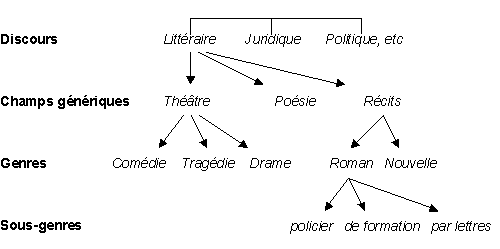
\includegraphics[width=0.8\textwidth]{img/MR_Genres1_niveau-declassification.png}
\caption{\textit{Niveau de classification défini par Rastier et Malrieu\footcites{rastier_malrieu_nodate}}}
\label{fig:rastier_marlrieu_niveau_classification}
\end{figure}


Marc Angenot, quant a lui propose une filiation générique du pamphlet sur des catégories essentiellement discursives. C'est ce que l'on peut observer avec la \textit{figure \ref{fig:angenot_niveau_inclusion_générique}}. Ces deux méthodes de classification du genre en ensemble et sous-ensemble montrent la richesse méthodologique et théorique de définition du genre littéraire.
\begin{figure}[H]
\centering %
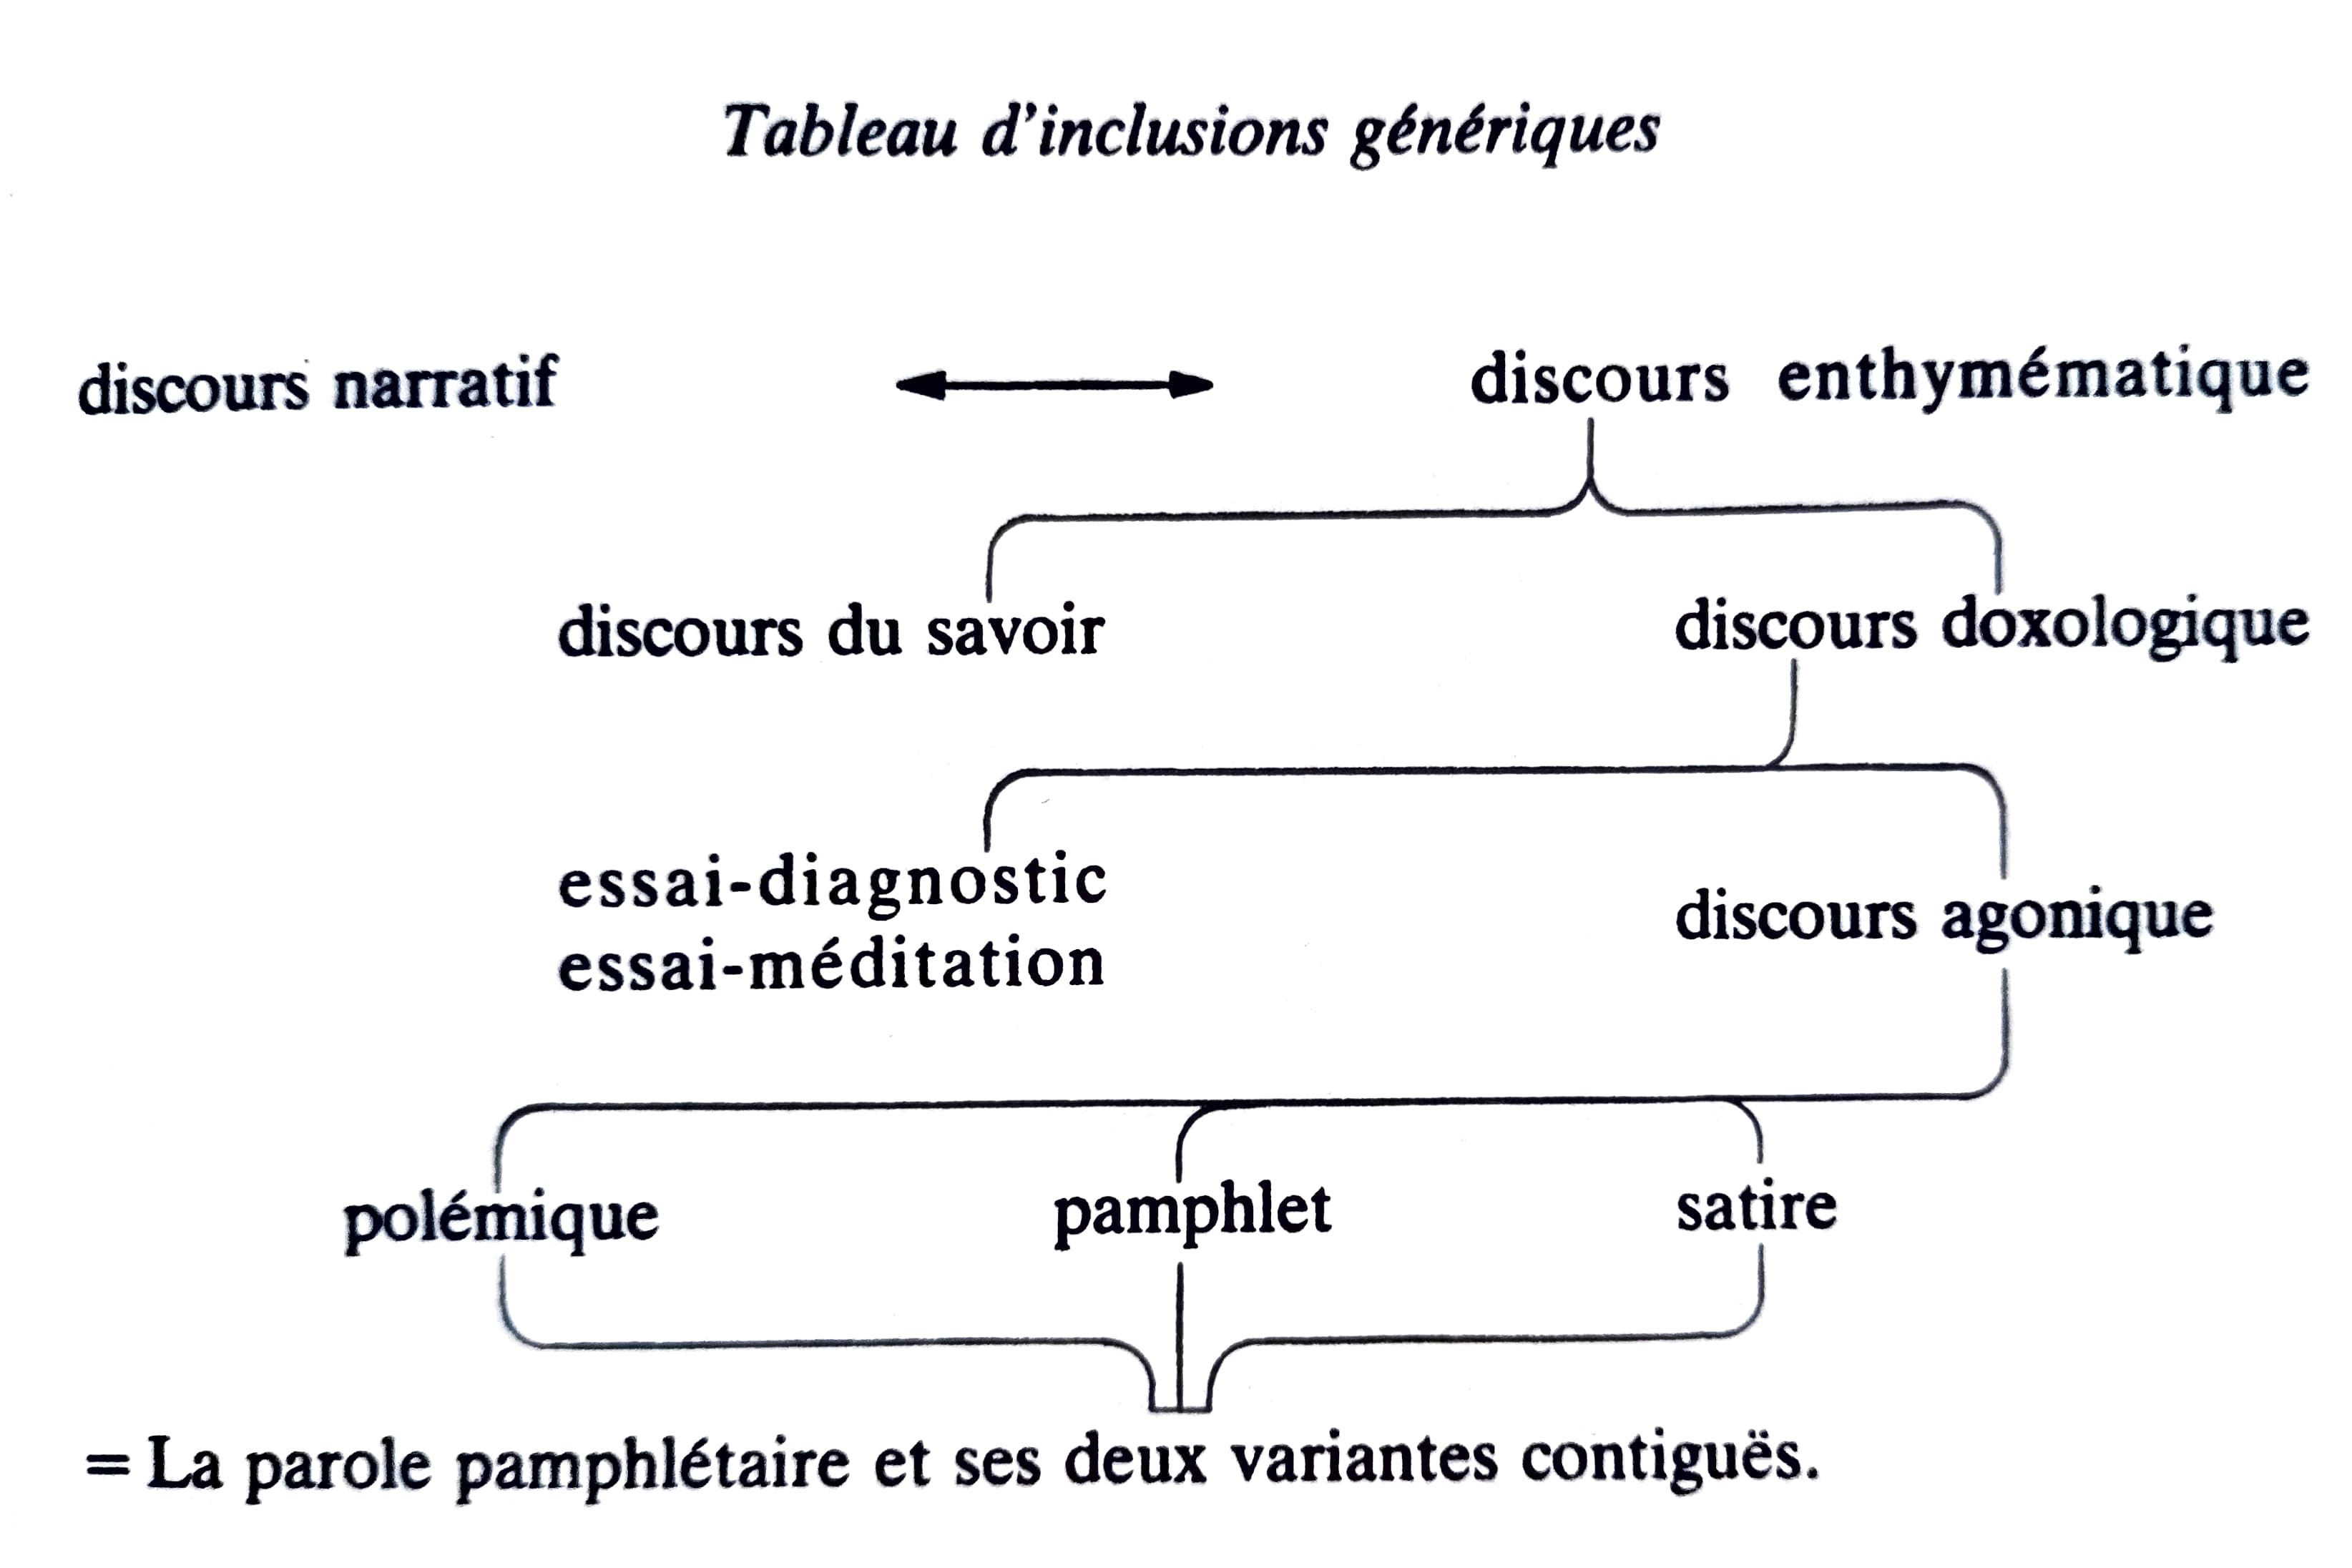
\includegraphics[width=0.65\textwidth]{img/fig_M_Angenot_tableau_inclusion_generique.png}
\caption{\textit{Niveau d'inclusion générique du pamphlet par Marc Angenot\footcites{angenot_parole_1982}}}
\label{fig:angenot_niveau_inclusion_générique}
\end{figure}
Ainsi nous observons le phénomène de genre comme catégorie s'insérant dans une hiérarchie d'ensemble. Une autre manière de définir le pamphlet peut passer par la définition d'un style collectif. Collectif à comprendre comme ensemble socioculturel, les pamphlétaires bien que ne se connaissant pas personnellement partagent un même air du temps. Marc Angenot d'ailleurs a dressé une typologie de la figure du pamphlétaire.
\section{Qu'est-ce-que le style ?}

La définition de la notion de style diffère en fonction du champ disciplinaire où l'on se place. Dans notre étude pluridisciplinaire nous empruntons la notion de style à la fois à la linguistique mais aussi à la stylométrie dont le mot même exprime l'étude de la mesure du style.
Notre recherche de traits formels spécifiques au \enquote{genre} pamphlétaire peux s'apparenter à une recherche d'un style collectif des textes étiquetés pamphlet. Rechercher des marques d'un style collectif suppose d'évincer les marques du style individuelle ou idiolecte. Si le style peut être compris comme \textit{la déviation d'une norme}, nous chercherons la norme de ces déviations dans les textes pamphlétaires. Notre approche de la notion de style est pluridisciplinaire et se situe au carrefour de la stylistique et de la stylométrie, une forme de linguistique de corpus appliqué avec de méthodes quantitatives. Dans la linguistique de corpus, le style est souvent défini comme la manière particulière dont un auteur ou un groupe d'auteurs utilise la langue pour communiquer, y compris les choix lexicaux, syntaxiques et sémantiques qui caractérisent leur production textuelle. Il peut être étudié à travers l'analyse de fréquences, de motifs récurrents, et d'autres caractéristiques linguistiques au sein de grands ensembles de textes. En stylométrie, le style se réfère aux propriétés linguistiques et statistiques distinctives qui permettent d'attribuer un texte à un auteur spécifique. Cette visée attributive nous intéresse particulièrement dans l'objectif d'une attribution non autoriale mais générique. En stylistique, le style se définit comme l'ensemble des choix linguistiques et stylistiques qu'un écrivain ou un locuteur fait pour s'exprimer de manière particulière. Cela inclut les aspects formels et expressifs de la langue, tels que la syntaxe, le vocabulaire, la ponctuation, les figures de style (métaphores, métonymies, etc.), et d'autres éléments qui contribuent à l'effet global du texte sur le lecteur ou l'auditeur. Nous prenons l'ensemble de ces notions pour étudier le style collectif des pamphlétaires comme la norme d'une déviation d'un champ générique qui se situe entre le style idiolectal et la catégorie de champ générique. 


\chapter{Objectifs et méthodes}

L'objectif de cette étude sera d'explorer avec des outils textométriques les spécificités discriminants le pamphlet, montrant en cela une stylistique propre du genre. Sur un large corpus étiqueté par auteurs et par genre nous déploierons des hypothèses stylistiques des procédés propres à la forme pamphlétaire, et appliquerons des méthodes quantitatives pour peser leur signification face aux autres genres de texte des mêmes auteurs pour extraire les traits spécifiques formels du pamphlet. Nous procéderons sur deux niveaux, à l'échelle des mots avec des méthodes de classification supervisé SVM et non supervisée avec une classification ascendante hiérarchique et une analyse en composantes principales, et à l'échelle de la phrase avec une analyse de l'énonciation et la recherche de motifs syntagmatiques génériques. Avec le déploiement de ces différentes focales et méthodes sur nos textes pamphlétaires nous espérons observer des composantes génériques suffisamment claires pour voir le pamphlet comme un genre.

\section{Constitution du corpus}

Pour mener à bien nos méthodes quantitatives, nous avons réuni des textes propres à constituer un échantillon assez représentatif des usages linguistiques écrits du pamphlet moderne. En linguistique de corpus, il existe une maxime comme quoi \enquote{Tout corpus reflète le point de vue qui a présidé à sa constitution}\footcites{rastier_malrieu_nodate}, nous tentons au maximum de réunir des textes de temporalité et de genre les plus proches possibles. Nous avons d'abord constitué un groupe d'écrivains reconnus pour avoir écrits des pamphlets : Claude Tillier, Paul-Louis Courier, Jules Vallès, Henri Rochefort, Léo Taxil, Auguste Chirac, Édouard Drumont, Zo d'Axa, Georges Darien, Octave Mirbeau, Maurice Barrès, Léon Bloy, Laurent Tailhade, Charles Péguy, Alphonse Daudet, Georges Bernanos, Louis-Ferdinand Céline. De la nous avons réuni le plus de texte numérisé possible pour chacun de ces écrivains. Par manque de quantité de texte par auteur, de cet ensemble nous avons du retrancher Claude Tillier, Paul-Louis Courrier, Henri Rochefort. Nous avons ensuite étiquetté chaque texte par date d'édition, par auteur et par genre. Nous aborderons par la suite les difficultés que cette étape de constitution d'un corpus a provoqué.

\subsection{Limites chronologiques}

Tout corpus reflète le point de vue qui a présidé à sa constitution : le nôtre a été réuni pour constituer un échantillon représentatif des usages linguistiques écrits du pamphlet.  Le cadre chronologique du corpus de cette étude va du Second Empire jusqu'à la fin de la seconde Guerre Mondiale, en cela il est plus restrictif que le corpus déployé par Marc Angenot qui lui propose de 1868 avec la parution de l'hebdomadaire \textit{La Lanterne}\footcites{rochefort_lanterne_1868} jusqu'à la révolte de mai 1968. Notre corpus est issu d'une conception intuitive et empire de ce qu'est le pamphlet d'après plusieurs acteurs de la critique ou de l'édition. La \textit{figure \ref{'fig:dates_editions'}} présente sous forme de boite à moustache la période de publication des auteurs du corpus en fonction des textes que nous avons pu intégrer au corpus et non la période absolue de publication. Il se compose de l'ensemble accessible de la production littéraire de treize écrivains dont chacun de leur ouvrage est catégorisé par un genre ou un ensemble.
\begin{figure}[H]
\centering %
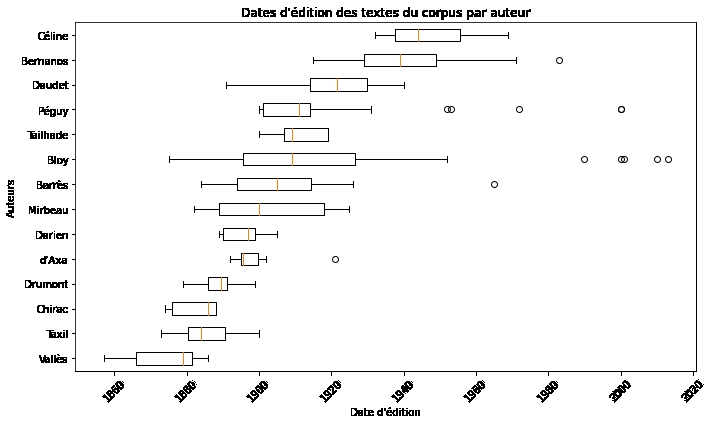
\includegraphics[width=0.85\textwidth]{img/M2_boxplot_corpus_chronologique.jpg}
\caption{\textit{Boite à moustache des dates d'éditions des textes du corpus par auteurs}}
\label{'fig:dates_editions'}
\end{figure}

Ces treize auteurs sont convoqués comme représentant la production pamphlétaire de cette période.  Ce choix est motivé par plusieurs facteurs : la pérennité de leur œuvre, la variété de leur idéologie et propos et l'impact de leur œuvre du vivant de ces écrivains. Ces facteurs restent difficilement mesurables, nous avons néanmoins essayé de représenter plusieurs sons de cloche de ce qu'a pu être la production littéraire pamphlétaire de cette période. 

De nombreuses difficultés n'ont pas pu être éliminés pour cette sélection de textes et la qualification en genre des textes. Une part importante de texte bien que qualifiée par différents acteurs (critiques, journalistes, éditeurs, encyclopédies, etc.) de pamphlet peut relever tout autant d'autres genres proches. Cela est en partie dû à l'ambiguïté et l'absence de définition clair du terme de pamphlet dans la recherche.
Une autre difficulté s'est ajouté pour la constitution de ce corpus quant à l'accessibilité des textes convoqués pour former ce corpus. La majorité des ouvrages sont issus de Wikisource, du projet Gutenberg, de Google Books et de Gallica. À l'exception des textes issus de Wikisource, l'ensemble des textes ont nécessités une étape laborieuse de traitement OCR (Optical Caracter Recognition) car uniquement disponible au format image. Cette conversion du format image au format texte s'est effectué sur les images des textes avec le logiciel Tesseract\footcites{noauthor_tesseract-ocrtesseract_nodate}. Une étape de préparation et de normalisation des images à été effectué avec l'utilitaire ScanTailor. \footcites{noauthor_4lex4scantailor-advanced_nodate}
Sur la figure suivante nous pouvons voir la part d'ouvrage réuni dans le corpus en rapport avec la production réelle identifiée de ces écrivains.
 \begin{figure}[H]
\centering %
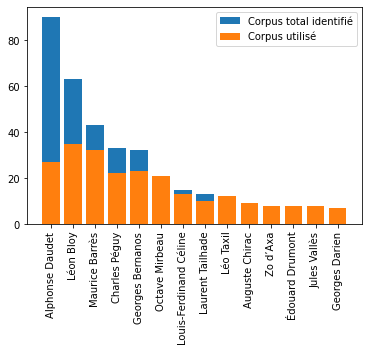
\includegraphics[width=0.85\textwidth]{img/barplot_corpus_auteurs.png}
\caption{\textit{Barplot des textes du corpus par auteurs sur le nombre total de textes identifié de l'auteur.}}
\end{figure}

\subsection{Limites génériques}

Nous avons identifié et réuni en catégorie générique large les différents textes du  corpus. Pour obtenir au maximum des catégories équilibrées, nous avons exclu les quelques pièces de théâtre et les recueils de poésie trop peu nombreux pour former une catégorie comparable aux autres. Cette production textuelle ce découpe en roman, nouvelle, intime, article, essai et pamphlet. Intime étant une catégorie regroupant des biographies, autobiographies et des mémoires. La catégorisation en genre des différents textes est basé sur l'état de l'art bien que certain textes puissent être qualifié par plusieurs étiquettes de genre, notamment certains essais et pamphlets qui sont parfois difficilement discernable les uns des autres sans une connaissance approfondi de leur contenu. Malgré ces difficultés nous avons donc un corpus cohérent de la production littéraire de nos auteurs pamphlétaires. La figure \ref{'fig:repartition_genre'} permet de visualiser le nombre de texte par catégorie générique et par auteur, montrant une distribution homogène, exception faite de la catégorie des nouvelles. 
 \begin{figure}[H]
\centering %
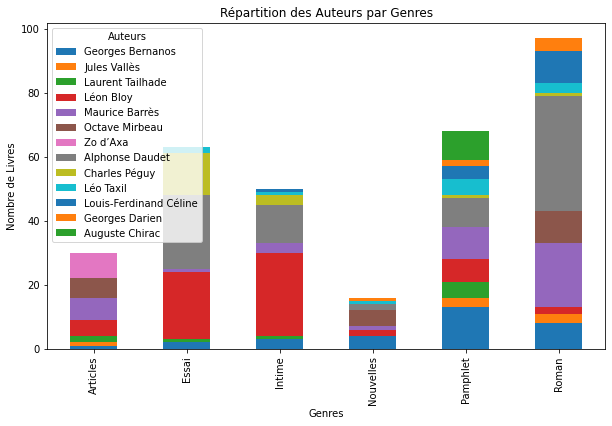
\includegraphics[width=0.65\textwidth]{img/barplot_corpus_genre.png}
\caption{\textit{Barplot de la répartition des auteurs par genre des textes du corpus}}
\label{'fig:repartition_genre'}
\end{figure}

\section{Conclusion}

Le corpus que nous avons constitué nous permettra à lui seul de déployer plusieurs méthodes quantitatives pour étudier le pamphlet. Sa constitution, bien que parfois elle ai nécessité des choix subjectifs et qu'elle soit dépendante de l'accessibilité imparfaite des ouvrages, fut le fruit d'un long travail de sélection des textes et des auteurs les plus représentatifs de la figure du pamphlétaire défini par Marc Angenot. Nous utilisons dans la première partie de cette étude un second corpus complémentaire issu de l'ANR Chapitres des romans du XIX\ieme et XX\ieme siècle, que nous définirons dans cette première partie.

%\footcites{guyot_stylemes_2006}
%\footcites{abbou_genre_2016}
%\footcites{bourdieu_les_1992}
%\footcites{marty_roland_2005}
%\footcites{molinie_style_1996}

%\footcites{molinie_approches_1993}

%\footcites{maingueneau_contexte_1993}

%\footcites{philippe_pourquoi_2021}
%\footcites{philippe_reve_2013}
%\footcites{barthes_degre_1972}
%\footcites{philippe_langue_2009}
%\footcites{jeannelle__2017}
%\footcites{molinie_quest-ce_1994}

%\footcites{angenot_glossaire_nodate}
\part{Approches générales stylométriques}

\chapter{Approche supervisé}

\section{Les Machines à vecteurs de support (SVM)}

Le terme de machines à vecteur de support se rapportent à un groupe d'algorithmes de classification basé sur l'apprentissage supervisé \footcites{noauthor_machine_2023}. 
Les SVM ont été largement utilisées dans divers domaines, y compris la classification de textes. Leur flexibilité pour traiter à la fois des séparations linéaires et non linéaires, ainsi que leur capacité à gérer des ensembles de données complexes avec de nombreuses dimensions, en font des outils puissants pour la classification et la régression dans le domaine de l'apprentissage automatique.
Les fondements des SVM ont été posés dans les travaux de Vladimir Vapnik et Alexey Chervonenkis des années 1960, qui ont développé la théorie de la dimension de Vapnik-Chervonenkis (VC-dimension). Cette théorie a permit à Vapnik avec son collègue Corinna Cortes, de formuler le concept de SVM dans les années 1990\footcites{cortes_support-vector_1995}. Leur objectif était de développer un algorithme d'apprentissage automatique capable de gérer des problèmes de classification complexes, notamment ceux impliquant des données non linéairement séparables. Ils ont introduit la notion d'hyperplan de marge maximale et ont développé des méthodes pour résoudre efficacement ce problème d'optimisation. Depuis les SVM ont rapidement gagné en popularité en tant qu'approche puissante pour la classification et la régression. Différentes variantes des SVM coexistent, y compris par l'utilisation de noyaux non linéaires pour traiter des données non séparables linéairement. Cela a conduit au développement de noyaux tels que le noyau gaussien (RBF) et le noyau polynomial qui ne nous intéresse pas particulièrement pour notre cas d'étude.

Depuis les années 2000, les SVM ont continué à évoluer avec l'avancée de la recherche en apprentissage automatique et en traitement du signal. Des variantes plus sophistiquées ont été développées pour aborder des tâches plus complexes, et des extensions ont été proposées pour la classification multi-classes et la régression. Malgré la concurrence qui existent avec de nouvelles approches, les SVM restent pertinentes et sont toujours utilisées pour des tâches de classification et de régression, en particulier lorsque les données sont en nombre limité ou lorsque l'interprétabilité du modèle est nécéssaire. Ils continuent de fournir une base théorique solide pour la compréhension de la complexité de l'apprentissage automatique et de la séparation des données. Les SVM comme classifieur de texte sont donc un choix judicieux du fait qu'ils gèrent facilement un très large nombre de dimensions, ce qui se produit avec une approche en n-grams de features.
Le choix de cet approche se trouve complémentaire des approches que nous déploierons ensuite au sens où, mise à part les choix du type de \textit{features} à extraire et la sélection des hyperparamètres de la SVM, l'ensemble ne dépend pas d'hypothèses inductives. C'est l'algorithme qui sélectionne de manière optimale les objets les plus discriminants pour définir nos classes génériques. En cela, il offre une entrée objectif pour définir des caractéristiques propres aux textes pamphlétaires.


En partant de données étiquetées en différentes classes, l'algorithme SVM cherche à maximiser des frontières entre chacune des classes fournies. Les SVM parviennent à accomplir cette tâche en exploitant des concepts géométriques et mathématiques. L'objectif principal est de trouver un hyperplan dans un espace de plusieurs dimensions. Cet hyperplan peut être linéaire (une simple ligne dans un espace bidimensionnel), mais les SVM peuvent également utiliser des fonctions de noyau pour projeter les données dans des espaces de dimensions supérieures, permettant ainsi de capturer des séparations non linéaires, ce qui est souvent le cas de données textuelles. Cette transformation permet aux SVM de gérer des problèmes de classification complexes et hautement dimensionnels. La notion de \enquote{marge} est cruciale dans les SVM. La marge est la distance entre l'hyperplan et les exemples de données les plus proches de chaque côté. L'objectif est de maximiser cette marge tout en minimisant les erreurs de classification. Les exemples de données qui se trouvent à la limite de la marge, et qui ont un impact sur la position de l'hyperplan, sont appelés \enquote{vecteurs de support}. Ce sont eux qui déterminent la position optimale de l'hyperplan en cherchant à maximiser la marge. 
Il est important de noter que les SVM peuvent également rencontrer des situations où les données ne peuvent pas être parfaitement séparées par un hyperplan. Dans ce cas, la SVM cherche un compromis en introduisant des marges d'erreur, ce qui est souvent désigné par le terme de \enquote{marges souples} (soft margins). Cela permet au modèle d'accepter un certain niveau d'erreur de classification tout en visant toujours à maximiser la marge.

\section{Méthode choisie}

Nous utilisons une implémentation de SVM déployée par Jean-Bapiste Camps nommée SuperStyl\footcites{camps_supervised_2021}. L'avantage de ce choix est de pouvoir facilement effectuer différentes variantes d'extraction de \textit{features} ainsi que différents entraînements en changeant aisément de paramètres et d'hyperparamètres.

Les SVM prennent en entrée non pas les textes eux-mêmes mais une matrice de caractéristiques issues des textes et de la classe à laquelle se rattache le texte. Ces caractéristiques sont les \textit{features} extraites des textes avec leurs occurrences. Une \textit{feature} dans ce contexte est une unité minimale qui couramment est choisie à l'échelle du caractère ou du mot. Pour évaluer la robustesse et la justesse d'un modèle et pour éviter le sous et le sur apprentissage, les SVM fonctionnent en deux temps, le premier sert à former le modèle et le second à vérifier sur de nouvelles données sa justesse.

Une option \textit{Hold-Out Validation} est de manuellement diviser les données en données d'entraînement et données de test. Les données d'entraînement servant à former le modèle en minisant sur ces données-ci ses erreurs, et les données de tests servants à vérifier la bonne généralisation du modèle de SVM ainsi formé. Le choix de la division du corpus de texte en données d'entraînement et de test étant à la discrétion du chercheur, traditionnellement on réserve entre 40\% et 30\% du corpus en données de test.

Il est possible d'augmenter la robustesse d'un modèle en faisant une \textit{cross validation}, c'est-à-dire une multiplication des entraînement et des tests où chaque donnée se sera retrouvée soit en entraînement soit en test dans une des multiples itérations.
Une autre option de division est le \textit{k-fold cross validation} où pour un nombre k, on divise les données en entraînement et en test k nombre de fois. 

Nous utilisons une autre méthode plus optimale sur nos données appelée \textit{leave-one-out cross validation}, cette méthode itérative va exclure de l'entraînement à chaque itération un texte de l'ensemble du corpus pour le fournir en donnée de test. Ainsi il y a autant d'entraînements et de tests que de texte dans le corpus. Cela correspond à un k-fold ou k est égale au nombre total de texte. L'estimation de la performance du modèle sera calculée par la moyenne des résultats sur les données tests. Cette option très robuste est aussi la plus coûteuse en ressource du fait de l'augmentation linéairement liée de ses itérations par rapport à la taille du corpus. C'est l'option que nous choisissons pour son gain de robustesse.

La première étape est de fournir des données cohérentes à l'algorithme de SVM. Nous passons pour chaque texte d'une chaîne de caractères à une représentation cohérente pour la classification. Le choix du contenu de cette représentation est l'étape d'extractions des \textit{features}. Plusieurs options s'offrent à nous. Nous ferons une extraction de \textit{features} par mots en trigrammes. Nous n'excluons pas des \textit{features} les mots outils \textit{ où stopwords} mais nous excluons la ponctuation ainsi que les caractères non alphabétique. Pour l'entrainement nous utiliserons un noyau linéaire, l'état de l'art en classification de textes avec une SVM considère que c'est le choix le plus approprié\footcites{kowalczyk_linear_2014}.

\chapter{Gestion du corpus pour l'approche supervisé SVM}

\section{Constitution de deux corpus}

Nous allons appliquer une extraction de \textit{features} et un entraînement de SVM sur deux corpus spécifiques. Le premier corpus permet de comparer les pamphlets à un ensemble de genre d'autres auteurs très divers pour vérifier l'aspect générique de nos pamphlets. Le second corpus est établi depuis l'ensemble de la production de nos auteurs pamphlétaire pour vérifier la force du signal générique vis-à-vis du signal autorial.

\subsection{Corpus de pamphlet face à d'autres genres d'autres auteurs}

Ce premier corpus est constitué des pamphlets de nos treize auteurs pamphlétaires mis ensemble avec des textes d'autres auteurs de genre distincts tels des romans, des mémoires et biographies et des nouvelles issus du Corpus ANR Chapitres : 2000romans19e20e constitué par l'unité de recherche THALIM 7172 \footcites{anrchapitres_anrchapitres2000romans19e20e_2022}. Il est constitué de 2033 romans francophones de 1813 au milieu du XX\ieme siècle au format xml:tei. Cette ressource est accessible sur Github\footcites{anrchapitres_anrchapitres2000romans19e20e_2023}, nous l'avons transformé au format plain-text en conservant les méta-données, telles que le genre, auteur et titre lorsque ces informations étaient accessibles.

L'intérêt de soumettre les pamphlets à d'autres genres et d'autres auteurs permet de créer un corpus très homogène et de réduire le signal autorial ou idiolecte en son sein. Il est homogène car nous avons accès à autant de texte que nous voulons depuis la base des 2000romans19e20e, ce qui n'est pas le cas de notre propre corpus de tous les textes (tous genres confondus) de nos pamphlétaires.

Pour constituer un corpus qui a du sens pour la SVM, nous partons de notre propre corpus de textes identifiés comme pamphlet et calculons la somme de mots et de caractères correspondants à cet ensemble. Avec cet étalon, nous sélectionnons aléatoirement dans le corpus ANR Chapitres un certains nombre de romans, de mémoires et biographies et de nouvelles qui respectent l'étalon fixé par le genre du pamphlet. C'est un problème d'optimisation ou nous souhaitons obtenir un nombre optimal de texte par genre respectant la contrainte où la somme de leur mots soit au plus proche de la somme des mots des textes pamphlets. Nous avons produit un code qui utilise la librairie \textit{pulp} en python qui résout ce problème d'optimisation linéaire où l'objectif est de sélectionner un certain nombre de fichiers par genre tout en respectant des contraintes sur la somme des caractéristiques des fichiers sélectionnés pour chaque genre. L'approche d'optimisation utilisée ici permet de choisir les fichiers de manière à maximiser le nombre total de fichiers tout en satisfaisant les contraintes imposées. La \textit{table \ref{'tab:corpus-mix-word'}} montrent cette répartition ou le nombre de texte par genre est inégal mais l'étalon de la somme des mots par genre est le plus homogène possible.
\begin{table}[H]
    \centering
    \begin{tabular}{lrrrrr}
    \toprule
    Genre & Nombre de texte & Somme & Min & Max & Moyenne  \\
    \toprule
    \midrule
    roman (ANR Chapitres) & 109 & 2939952 & 681 & 38207 & 26972.03 \\
    \midrule
    mémoire et biographie (ANR Chapitres) & 92 & 2951061 & 1399 & 45185 & 32076.75 \\
    \midrule
    nouvelle (ANR Chapitres) & 141 & 2935918 & 844 & 41442 & 20822.11 \\
    \midrule
    pamphlet & 48 & 2931562 & 2356 & 263090 & 61074.20 \\
    \bottomrule
    \end{tabular}
    \caption{Corpus 1 par genre et par proportion de mots}
    \label{'tab:corpus-mix-word'}
\end{table}

 Sur ce premier corpus constitué nous effectuons un échantillonage par 10000 mots pour obtenir un corpus homogène au niveau de la moyenne de mots par texte par genre. Nous choisissons ce pas de 10000 car il correspond plus au moins au dixième-vingtième des moyenne par texte par genre, ce qui nous assure d'un nombre d'échantillon élevé mais non trop copieux en ressource pour l'entraînement. La \textit{table \ref{'tab:corpus-mix-echantillons-word'}} vous présentent le résultat de cet échantillonnage. Nous remarquons que chaque moyenne par genre de la longueur des textes par mots est homogénéisée grâce à la division des textes en échantillons de 10000 mots, la conséquence évidente est l'augmentation du nombre de \textit{textes} par genre représentant des fractions de 10000 mots de chacun des textes précédents.

\begin{table}[H]
    \centering
    \begin{tabular}{lrrrrr}
    \toprule
    Genre & Nombre de texte & Somme & Min & Max & Moyenne  \\
    \toprule
    \midrule
    roman & 243 & 2939952 & 681 & 19819 & 12098.56 \\
    \midrule
    mémoire et biographie & 256 & 2951061 & 1399 & 19988 & 11527.58 \\
    \midrule
    nouvelle & 272 & 2935918 & 844 & 19984 & 10793.81 \\
    \midrule
    pamphlet & 277 & 2931562 & 2356 & 19970 & 10583.25 \\
    \bottomrule
    \end{tabular}
    \caption{Corpus 1 échantillonné par genre et par proportion de mots}
    \label{'tab:corpus-mix-echantillons-word'}
\end{table}

C'est ce corpus nouvellement constitué le plus homogène possible que nous appliquerons l'extraction des \textit{features}. Nous choisissons d'appliquer une extraction par unigramme de mots. Nous entraînons la SVM avec un noyau LinearSVC en cross-validation Leave-one-out avec le paramètre class-weights bien que le corpus nouvellement constitué soit particulièrement homogène.

\subsection{Corpus uniquement composé de différents genres des auteurs pamphlétaires}

Le second corpus est simplement l'ensemble des textes de nos pamphlétaires classés par genre ou grands ensembles génériques tel que des essais, des pamphlets, des mémoires et biographies, des articles et des romans, la \textit{table \ref{'tab:corpus-word'}} présente de la même manière que pour le corpus précédent la répartition des mots par genre.
L'intérêt du second corpus soumis à la SVM est de vérifier que le signal générique puisse être suffisamment spécifique pour que la SVM identifie le pamphlet comme une classe pertinente de catégorisation malgré un signal autorial fort (tous les textes se divisent alors seulement entre 13 auteurs). Et cela alors que nous sommes limité par notre corpus en nombre de textes par genre, ce qui rend se corpus bien moins homogène que le premier.
Il n'est pas possible d'espérer uniformiser la somme des mots par genre dans ce cas présent car nous ne souhaitons pas exclure des textes pour y parvenir étant donné qu'ils représentent l'ensemble des textes que nous avons réussi à identifier de nos auteurs pamphlétaires.

\begin{table}[H]
    \centering
    \begin{tabular}{lrrrrr}
    \toprule
    Genre & Nombre de texte & Somme & Min & Max & Moyenne  \\
    \toprule
    \midrule
    roman & 78 & 5702861 & 1450 & 284630 & 73113.60 \\
    \midrule
    mémoire et biographie & 13 & 757025 & 6043 & 88988 & 58232.69 \\
    \midrule
    article & 25 & 473482 & 570 & 114731 & 18939.28 \\
    \midrule
    essai & 37 & 2527073 & 2108 & 819600 & 68299.27 \\
    \midrule
    pamphlet & 48 & 2931562 & 2356 & 263090 & 61074.20 \\
    \bottomrule
    \end{tabular}
    \caption{Corpus 2 par genre et par proportion de mots}
    \label{'tab:corpus-word'}
\end{table}

Ce second corpus va lui aussi subir un échantillonage des textes tout les 10000 mots, cela permettra une certaine homogénéisation de la moyenne des mots par texte que l'on peut observer sur la \textit{table \ref{'tab:corpus-mix-echantillons-word'}}. Certaines classes se retrouvent sur représentées mais nous comptons sur l'hyperparamètre class\_weights implémenté dans \textit{Superstyl} pour appliquer un poids à chaque classe permettant de rétablir un équilibrage entre elles.

\begin{table}[H]
    \centering
    \begin{tabular}{lrrrrr}
    \toprule
    Genre & Nombre de texte & Somme & Min & Max & Moyenne  \\
    \toprule
    \midrule
    roman & 542 & 5702861 & 1450 & 19967 & 10521.88 \\
    \midrule
    mémoire et biographie & 70 & 757025 & 6043 & 18988 & 10814.64 \\
    \midrule
    article & 56 & 473482 & 570 & 18900 & 8455.03 \\
    \midrule
    essai & 239 & 2527073 & 2108 & 19600 & 10573.52 \\
    \midrule
    pamphlet & 277 & 2931562 & 2356 & 19970 & 10583.25 \\
    \bottomrule
    \end{tabular}
    \caption{Corpus 2 par genre et par proportion de mots}
    \label{'tab:corpus-echantillon-word'}
\end{table}

\section{Résultats et analyse de la SVM sur chacun des corpus}

Pour chacun des deux corpus, la SVM produit des métriques et différentes données propre à indiquer la pertinence de la classification ainsi que les réussites et les échecs des prédictions de chaque texte par classe. La sortie de l'entraînement de \textit{Superstyl}, l'implémentation de la SVM que nous utilisons donne à voir cinq métriques distinctes qui chacune éclaire notre compréhension de la pertinence du classifieur sur nos données. Ces métriques sont prédéfinies au sens de l'implémentation de \textit{SuperStyl}.

Précision :\\
La précision mesure la proportion de prédictions positives faites correctement par le modèle parmi toutes les prédictions positives qu'il a effectuées. Une haute précision indique que le modèle a tendance à être prudent lorsqu'il prédit l'appartenance d'un texte à une classe.

\begin{equation}
Pr\acute{e}cision = \frac{Vrais Positifs}{Vrais Positifs + Faux Positifs}
\end{equation}

Rappel (ou Sensibilité) :\\
Le rappel mesure la proportion de prédictions positives correctes parmi toutes les instances réellement positives. Un rappel élevé indique que le modèle a la capacité de détecter la plupart des textes appartenant à une classe.

\begin{equation}
Rappel = \frac{Vrais Positifs}{Vrais Positifs + Faux N\acute{e}gatifs}
\end{equation}

F1-score :\\
Le F1-score est une métrique qui combine à la fois la précision et le rappel en une seule valeur. Cela est particulièrement utile lorsque qu'il faut équilibrer la précision et le rappel, car ces deux mesures peuvent être en conflit. Le F1-score est la moyenne harmonique de la précision et du rappel, ce qui permet de donner plus de poids aux valeurs basses. Un F1-score élevé indique un bon équilibre entre la précision et le rappel.

\begin{equation}
F1-score = \frac{2 \times (Pr\acute{e}cision \times Rappel)}{Pr\acute{e}cision + Rappel}
\end{equation}

Accuracy (Précision globale) :\\
L'accuracy mesure la proportion de prédictions correctes (positives et négatives) faites par le modèle parmi toutes les prédictions. C'est la métrique la plus simple, mais elle peut être trompeuse lorsque les classes sont déséquilibrées. Par exemple, si nous avons une classe très majoritaire, un modèle prédisant toujours cette classe obtiendra une bonne \textit{accuracy} même s'il ne prédit jamais l'autre classe.

\begin{equation}
Accuracy = \frac{Vrais Positifs + Vrais N\acute{e}gatifs}{Total\quad des\quad instances}
\end{equation}

Macro-Average :\\
Le macro-average est une métriques pour calculer des mesures comme la précision, le rappel et le F1-score de l'ensemble de nos classes. C'est la moyenne non pondérée sur toutes les classes pour une métrique donnée. Cela garantit que chaque classe est traitée avec la même importance, indépendamment de sa taille.

\begin{equation}
Macro-Average = \frac{\sum_{chaque\quad classe} (M\acute{e}trique\quad pour\quad la\quad classe)}{Nombre\quad total\quad de\quad classes}
\end{equation}


Weighted-Average :\\
 Contrairement au macro-average, le weighted-average prend en compte le déséquilibre des classes. Il calcule la moyenne des métriques en fonction de la distribution des classes. Les classes avec plus d'instances ont un poids plus élevé dans le calcul de la moyenne, tandis que les classes moins représentées ont un poids plus faible.

\begin{equation}
Weighted-Average = \frac{\sum_{chaque\quad classe} (M\acute{e}trique\quad de\quad la\quad classe \times Poids\quad de\quad la\quad classe)}{Nombre\quad total\quad d'instances}
\end{equation}

En plus de ces métriques nous pouvons analyser la matrice de confusion indiquant le nombre de texte par classes véridiques et par classes prédites. Mais aussi le tableau des textes mal attribués avec leur classe réelle et leur classe prédite. Et enfin un diagramme à barres par des classes indiquant les \textit{features} significatives et leur coefficients. L'ensemble de ces métriques, tableaux et graphiques permettent au mieux de comprendre la pertinence et la robustesse du classifieur.

\subsection{Sortie du Corpus 1}
Pour notre corpus de texte issu de l'ANR Chapitres et de notre ensemble de textes pamphlétaires, nous constatons que le genre du pamphlet est la classe la mieux identifiée. Les métriques générales de l'accuracy, macro-average et weighted average montrent que le modèle produit 20\% d'erreur toutes classes confondues. Nos trois classes roman, mémoire et biographie et nouvelle sont celles qui ont le plus de mal à être identifiée de manière indépendante. Cela tient probablement à leur proximité de champ générique là où la classe pamphlet est pleinement distingué. Sur la \textit{table \ref{'tab:matriceconfusioncorpus1'}} nous constatons que seule deux échantillons de la classe pamphlet sont identifiés comme appartenant à une autre classe, en l'occurrence mémoire et biographie. La table des mauvaises attributions, \textit{table \ref{tab:misattributions-corpus1}}, indique qu'il s'agit du premier échantillon de 10000 mots de \textit{Bagatelles pour un massacre} de Louis-Ferdinand Céline et de \textit{La Noire Idole} de Laurent Tailhade. La première mauvaise attribution est composé du passage de la présentation du premier ballet par le narrateur, \textit{La Naissance d'une fée}. La seconde mauvaise attribution est aussi un cas limite en cela qu'elle porte en elle une grande part de narration de petites histoires sur la prise d'opioïde par les grands du monde. 
D'autres cas limites apparaissent dans les mauvaises attributions tel que des échantillons d'\textit{Aden Arabie} de Paul Nizan qui porte des passages souvent qualifiés de pamphlétaires.

\begin{table}[H]
    \centering 
    \begin{tabular}{l c c c c}
        \toprule
             & precision & recall & f1-score & support \\
        \toprule
        \midrule
        roman & 0.81 & 0.75 & 0.78 & 243 \\
        \midrule
        mémoire et bio. & 0.71 & 0.70 & 0.70 & 256\\
        \midrule
        nouvelle & 0.72 & 0.74 & 0.73 & 272\\
        \midrule
        pamphlet & 0.94 & 0.99 & 0.97 & 277\\
        \midrule
        & & & & \\
        \midrule
        accuracy & & & \textbf{0.80} & 1048 \\
        \midrule
        macro-average & 0.80 & 0.80 & 0.80 & 1048\\
        \midrule
        weighted average & 0.80 & 0.80 & 0.80 & 1048\\

        \bottomrule
    \end{tabular}
\caption{Sortie de la SVM sur corpus 1 échantillonné, 3-mots, LOOCV}
\label{'tab:SVMcorpus1'}
\end{table} 

\begin{table}[H]
    \centering 
    \begin{tabular}{|c|l|c|c|c|c|}
        \hline
        \multicolumn{2}{|c|}{} & \multicolumn{4}{c|}{Prédiction} \\
        \cline{3-6}
        \multicolumn{2}{|c|}{} & roman & mémoire et bio. & nouvelle & pamphlet \\
        \hline
        & roman & 183 & 24 & 34 & 2 \\
        \cline{2-6}
        \multirow{3}*{Vrai} & mémoire et bio. & 22 & 179 & 42 & 13 \\
        \cline{2-6}
        & nouvelle & 22 & 48 & 200 & 2 \\
        \cline{2-6}
        & pamphlet & 0 & 2 & 0 & 275 \\
        \hline
    \end{tabular}
\caption{Matrice de confusion du corpus 1 échantillonné}
\label{'tab:matriceconfusioncorpus1'}
\end{table}
La Matrice de confusion présente dans la \textit{table \ref{'tab:matriceconfusioncorpus1'}} permet d'observer la répartition des erreurs de classification qui est assez homogène entre les classes excepté pour la classe pamphlet où très peu d'échantillons de cette classe se retrouve mal classé et peu d'échantillon d'autres classes se retrouvent classés en pamphlet.

\begin{figure}[H]
\centering %
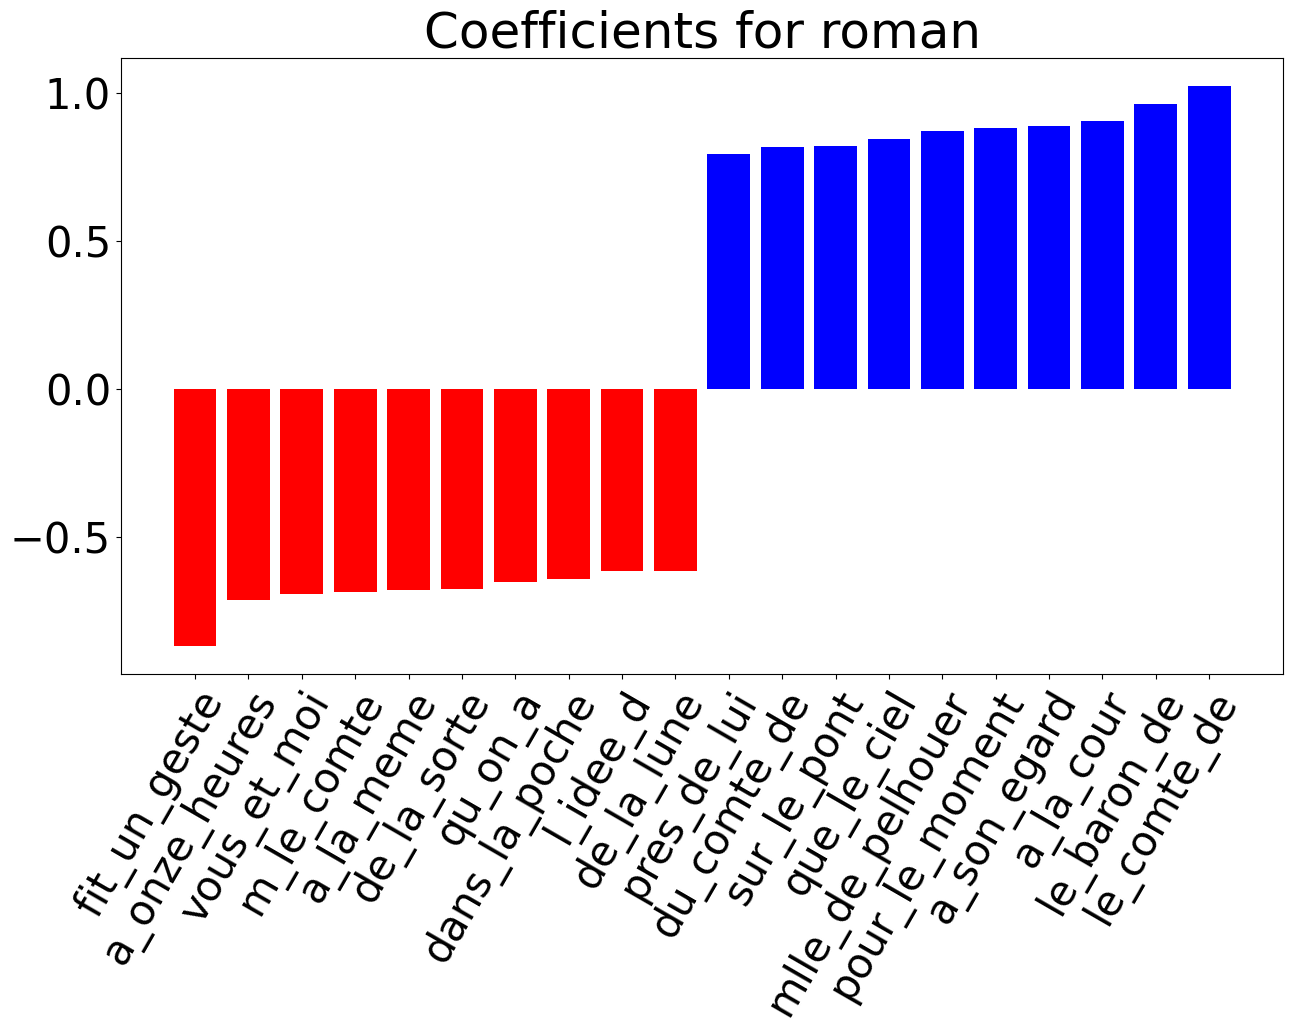
\includegraphics[width=0.70\textwidth]{img/coefs-corpus1-roman.png}
\caption{\textit{Diagramme à barres des coefficients de la classe roman du corpus 1}}
\label{'fig:coefs-corpus1-roman'}
\end{figure}

\begin{figure}[H]
\centering %
\includegraphics[width=0.70\textwidth]{img/coefs-corpus1-mémoire et bio..png}
\caption{\textit{Diagramme à barres des coefficients de la classe mémoire et biographie du corpus 1}}
\label{'fig:coefs-corpus1-mémoire et bio.'}
\end{figure}

\begin{figure}[H]
\centering %
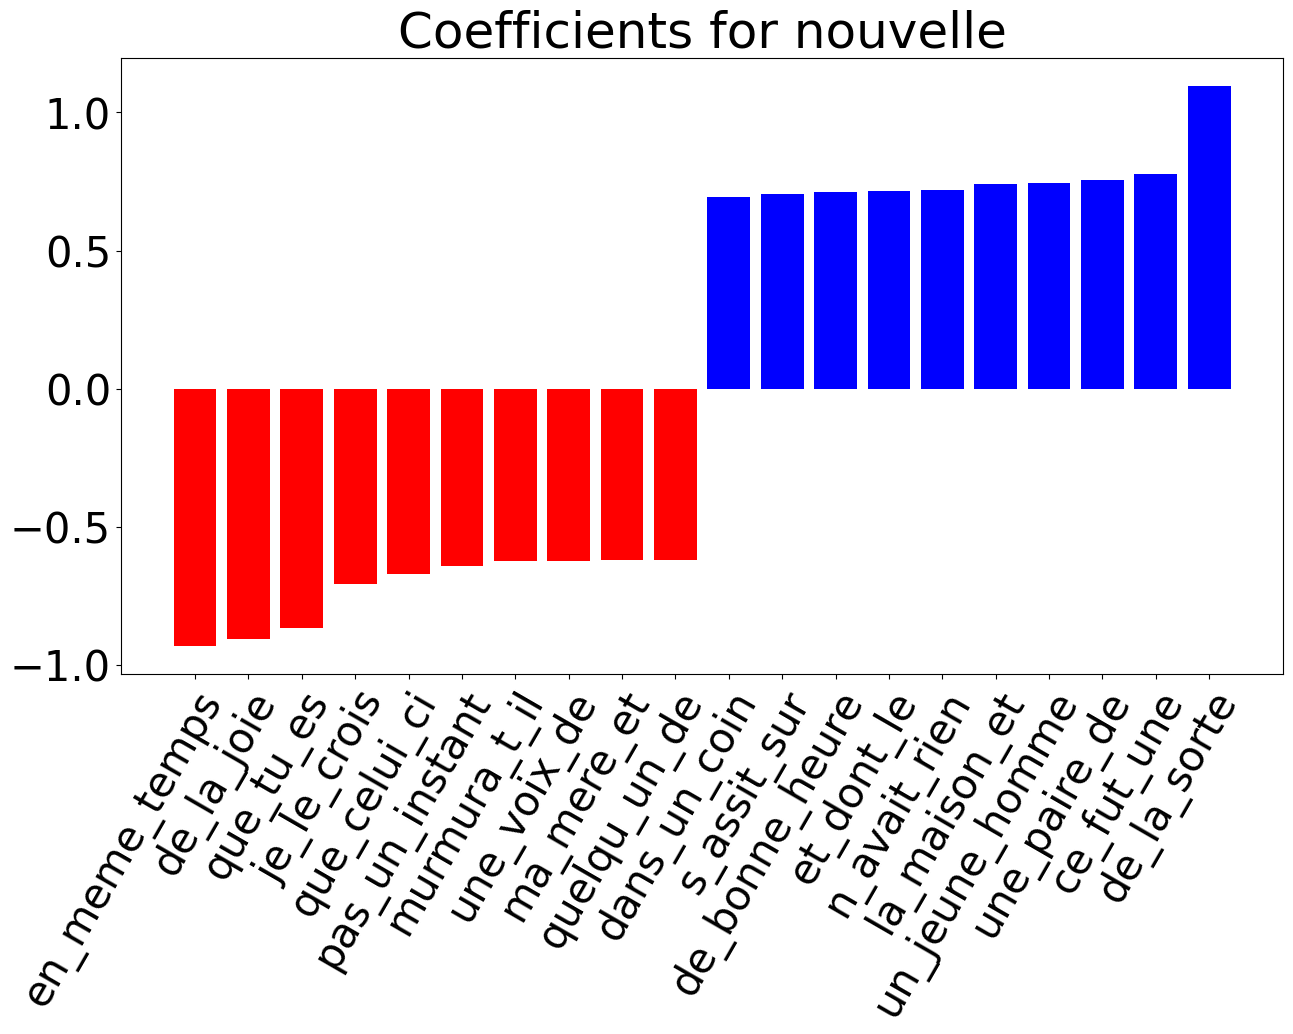
\includegraphics[width=0.70\textwidth]{img/coefs-corpus1-nouvelle.png}
\caption{\textit{Diagramme à barres des coefficients de la classe nouvelle du corpus 1}}
\label{'fig:coefs-corpus1-nouvelle'}
\end{figure}

\begin{figure}[H]
\centering %
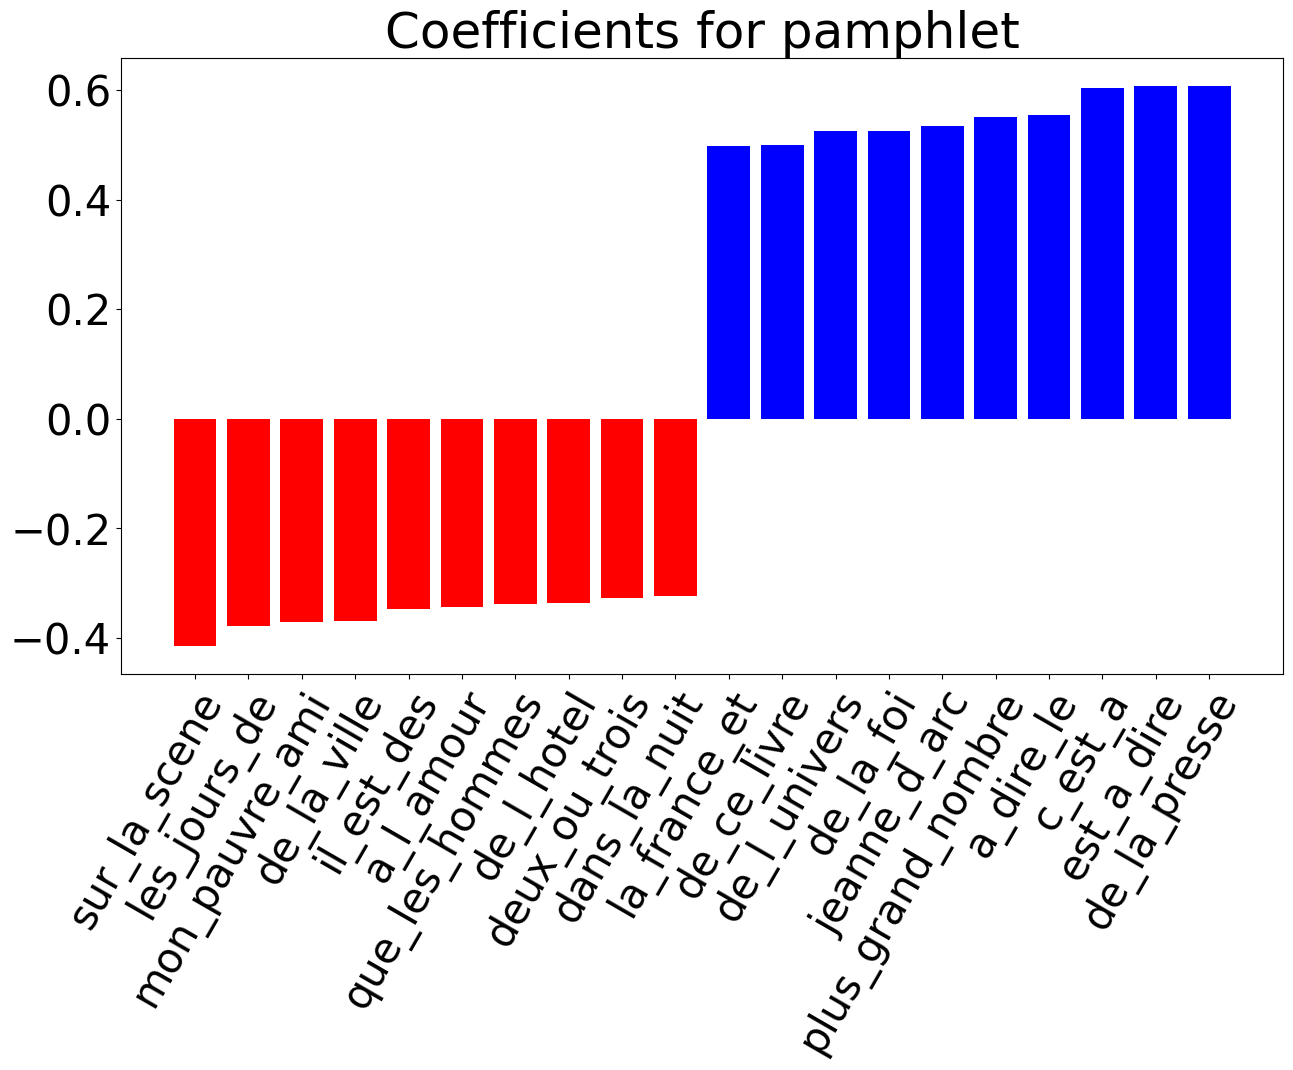
\includegraphics[width=0.70\textwidth]{img/coefs-corpus1-pamphlet.png}
\caption{\textit{Diagramme à barres des coefficients de la classe pamphlet du corpus 1}}
\label{'fig:coefs-corpus1-pamphlet'}
\end{figure}

Au niveau des diagrammes à barres des coefficients des classes du roman, de la nouvelle et des mémoires et biographies, nous pouvons regrouper plusieurs trigrammes de mots en groupes distincts. Le principale problème pour analyser ces fragments de proposition est qu'ils dépendent d'un contexte que nous ne pouvons observer ici. Nous regroupons en un champ générique les trois classes de mémoire et bio., roman et nouvelle en différents type de trigramme. Les trigrammes relatifs à la narration et à la description :
\enquote{\textit{près de lui}} (Roman), \enquote{\textit{sur le pont}} (Roman), \enquote{\textit{pour le moment}} (Roman), \enquote{\textit{dans un coin}} (Nouvelle), \enquote{\textit{s'assit sur}} (Nouvelle), \enquote{\textit{de bonne heure}} (Nouvelle).
Lest trigrammes liés aux personnages et aux titres de noblesse :
\enquote{\textit{mlle de pelhouer}} (Roman), \enquote{\textit{le baron de}} (Roman), \enquote{\textit{le comte de}} (Roman), \enquote{\textit{m le comte}} (Mémoire), \enquote{\textit{un jeune homme}} (Nouvelle), \enquote{\textit{du comte de}} (Roman).
Les trigrammes indiquant une proximité géographique ou spatiale :
\enquote{\textit{dans un coin}} (Nouvelle), \enquote{\textit{s'assit sur}} (Nouvelle), \enquote{\textit{hôtel de ville}} (Mémoire).
Les trigrammes indiquant une heure spécifique ou une durée :
\enquote{\textit{pour le moment}} (Roman), \enquote{\textit{de bonne heure}} (Nouvelle).
Les trigrammes relatifs à la connaissance et à l'expérience personnelle :
\enquote{\textit{tu ne sais}} (Mémoire), \enquote{\textit{il m'était}} (Mémoire).
Un trigramme indiquant des quantités approximatives :
\enquote{\textit{deux ou trois}} (Mémoire).
Un trigramme indiquant une observation ou un événement :
\enquote{\textit{on a vu}} (Mémoire).
Un trigramme exprimant une manière ou un processus :
\enquote{\textit{de la sorte}} (Nouvelle). Pour ces trois classes les trigrammes indiquent bien une réalité générique narrative sous-jacente.

Quand à la classe pamphlet nous divisons les trigrammes en quatre catégories. Les trigrammes liés à des thèmes spécifiques :
\enquote{\textit{la france et}}, \enquote{\textit{de ce livre, de l'univers}}, \enquote{\textit{de la foi}}, \enquote{\textit{jeanne d'arc}}.
Les trigrammes introduisant une déclaration ou une clarification :
\enquote{\textit{à dire le}}, \enquote{\textit{c'est à dire}}.
Un trigramme lié aux médias et à la communication :
\enquote{\textit{de la presse}} et un trigramme indiquant une généralisation ou une quantité :
\enquote{\textit{plus grand nombre}}

Nous espérions trouver dans les trois classes mémoire, roman et nouvelle des verbes d'incises qui distinguassent mieux ce champ générique de celui du pamphlet mais tel n'en fut pas le cas. Nous observons au-delà des thèmes qu'ouvrent les trigrammes, des trigrammes propres à une écriture argumentative, ce qui semble bien distinguer le champ générique de la narration du pamphlet plus proche de l'essai argumentatif. Les thèmes capturés par la SVM pour le pamphlet le distingue bien des autres classes. Il est notable d'observer la présence de Jeanne d'Arc qui est une figure de référence pour la plupart des pamphlétaires mais aussi les enjeux de patriotisme et de religion.




\subsection{sortie du Corpus 2}

Ce second corpus constitué uniquement des textes des auteurs pamphlétaires donne des résultats supérieurs en terme d'accuracy globale, chaque classe étant globalement mieux reconnue (\textit{table \ref{'tab:SVMcorpus2'}}) même si la classe pamphlet a un f1-score légèrement inférieur à celui du premier corpus. Nous sommes particulièrement surpris qu'il y ai une si bonne distinction entre la classe pamphlet et celle de l'essai, leur proximité de champ générique ajouté à la force du style autorial nous laissait à penser qu'ils s'interférassent l'un l'autre plus profondément. C'est la classe article qui donne la moins bonne classification, la principale cause peut être la faiblesse de sa consistance en terme de taille, mais il semble possible que la proximité du signal autorial puisse brouiller la classification.

\begin{table}[H]
    \centering 
    \begin{tabular}{l c c c c}
        \toprule
             & precision & recall & f1-score & support \\
        \toprule
        \midrule
        roman & 0.92 & 0.96 & 0.94 & 542 \\
        \midrule
        mémoire et biographie & 0.94 & 0.86 & 0.90 & 70\\
        \midrule
        article & 0.76 & 0.68 & 0.72 & 56\\
        \midrule
        essai & 0.83 & 0.88 & 0.85 & 239\\
        \midrule
        pamphlet & 0.91 & 0.83 & 0.87 & 277\\
        & & & & \\
        \midrule
        accuracy & & & \textbf{0.89} & 1184 \\
        \midrule
        macro-average & 0.87 & 0.84 & 0.85 & 1184\\
        \midrule
        weighted average & 0.89 & 0.89 & 0.89 & 1184\\

        \bottomrule
    \end{tabular}
\caption{Sortie de la SVM sur corpus 2 échantillonné, 3-mots, LOOCV, class-weight}
\label{'tab:SVMcorpus2'}
\end{table} 

\begin{table}[H]
    \centering 
    \begin{tabular}{|c|l|c|c|c|c|c|}
        \hline
        \multicolumn{2}{|c|}{} & \multicolumn{5}{c|}{Prédiction} \\
        \cline{3-7}
        \multicolumn{2}{|c|}{} & roman & mémoire et bio. & article & essai & pamphlet \\
        \hline
        & roman & 518 & 3 & 1 & 17 & 3 \\
        \cline{2-7}
        \multirow{3}*{Vrai} & mémoire et bio. & 7 & 60 & 1 & 1 & 1 \\
        \cline{2-7}
        & article & 9 & 0 & 38 & 2 & 7 \\
        \cline{2-7}
        & essai & 12 & 0 & 4 & 211 & 12 \\
        \cline{2-7}
        & pamphlet & 16 & 1 & 6 & 24 & 230 \\
        \hline
    \end{tabular}
    \caption{Matrice de confusion du corpus 2 échantillonné}
    \label{'tab:matriceconfusioncorpus2'}
\end{table}

\begin{figure}[H]
\centering %
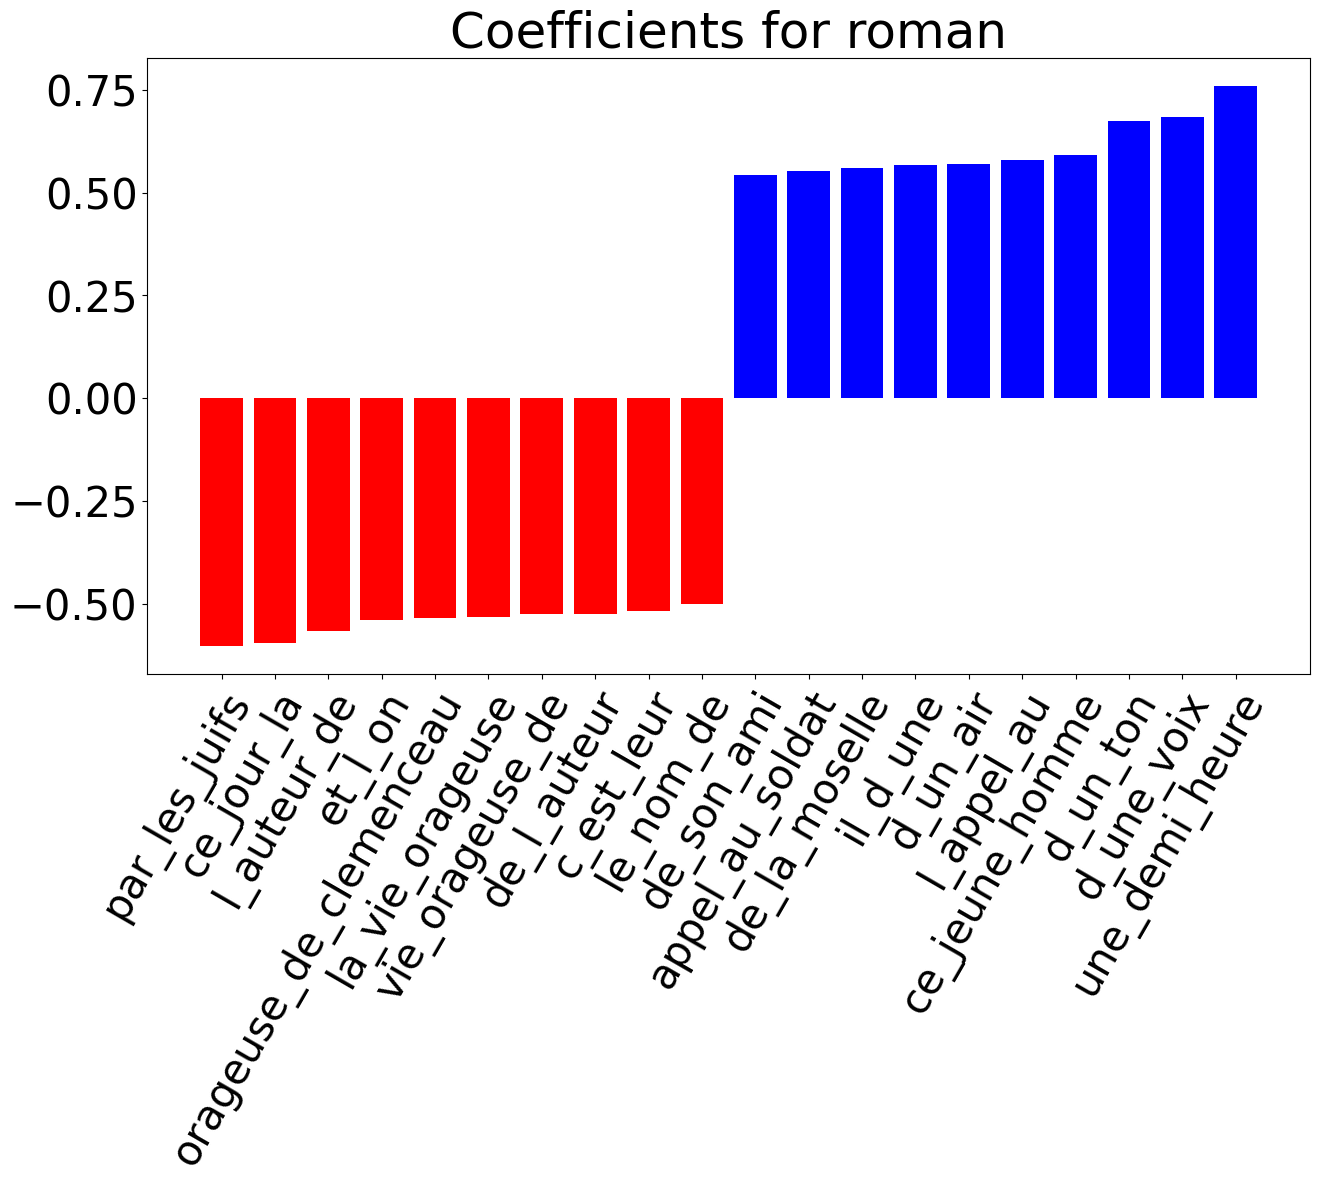
\includegraphics[width=0.70\textwidth]{img/coefs-corpus2-roman.png}
\caption{\textit{Diagramme à barres des coefficients de la classe roman du corpus 2}}
\label{'fig:coefs-corpus2-roman'}
\end{figure}

\begin{figure}[H]
\centering %
\includegraphics[width=0.70\textwidth]{img/coefs-corpus2-mémoire et bio..png}
\caption{\textit{Diagramme à barres des coefficients de la classe mémoire et biographie du corpus 2}}
\label{'fig:coefs-corpus2-mémoire et bio.'}
\end{figure}

\begin{figure}[H]
\centering %
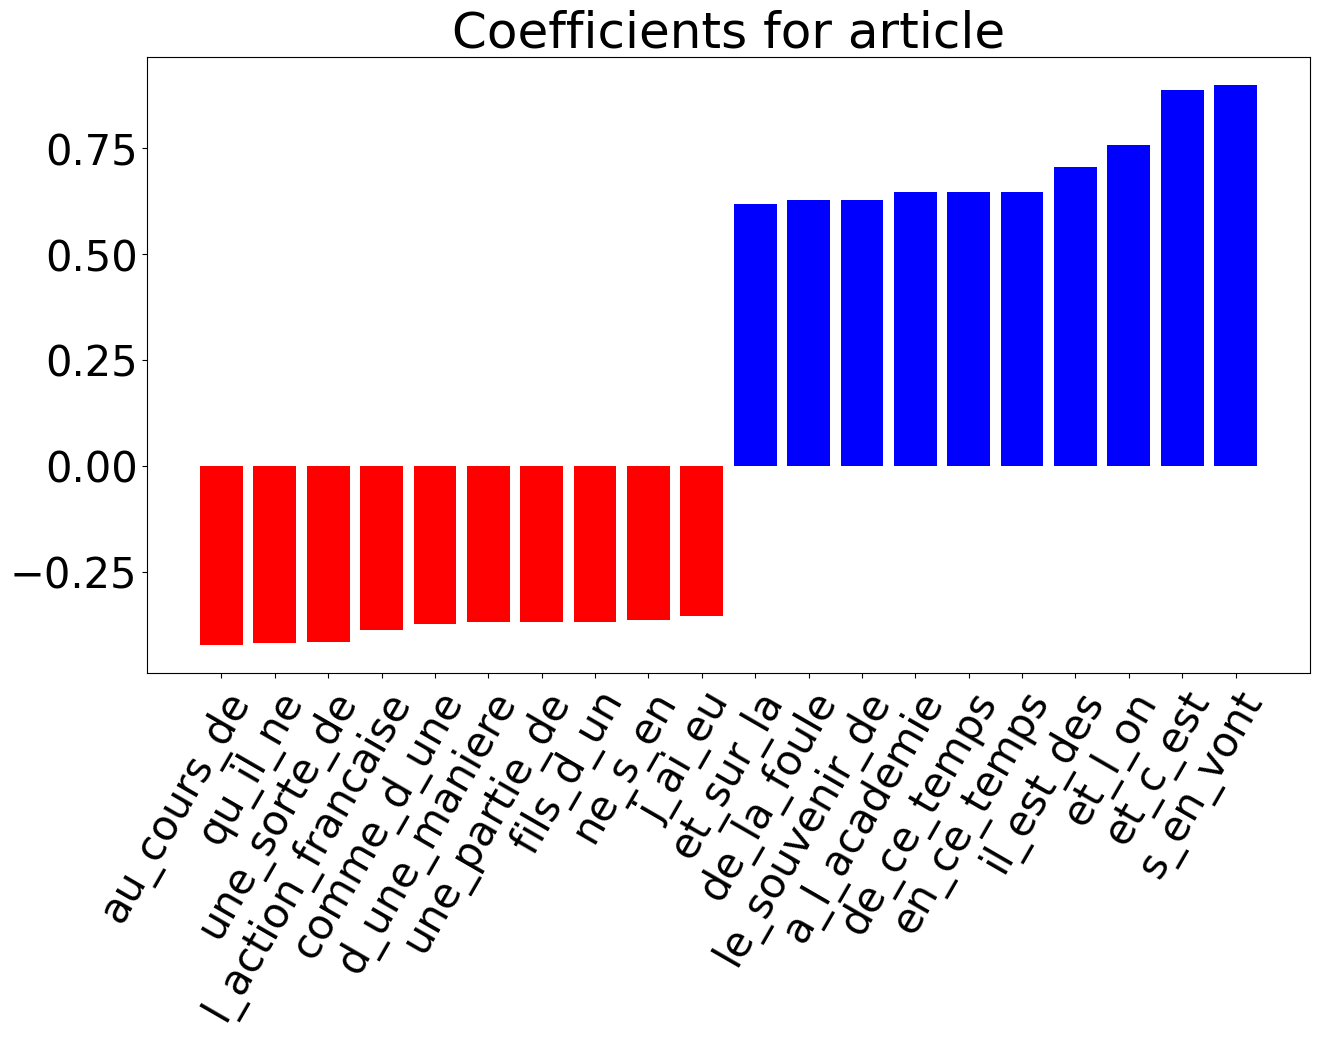
\includegraphics[width=0.70\textwidth]{img/coefs-corpus2-article.png}
\caption{\textit{Diagramme à barres des coefficients de la classe article du corpus 2}}
\label{'fig:coefs-corpus2-article'}
\end{figure}

\begin{figure}[H]
\centering %
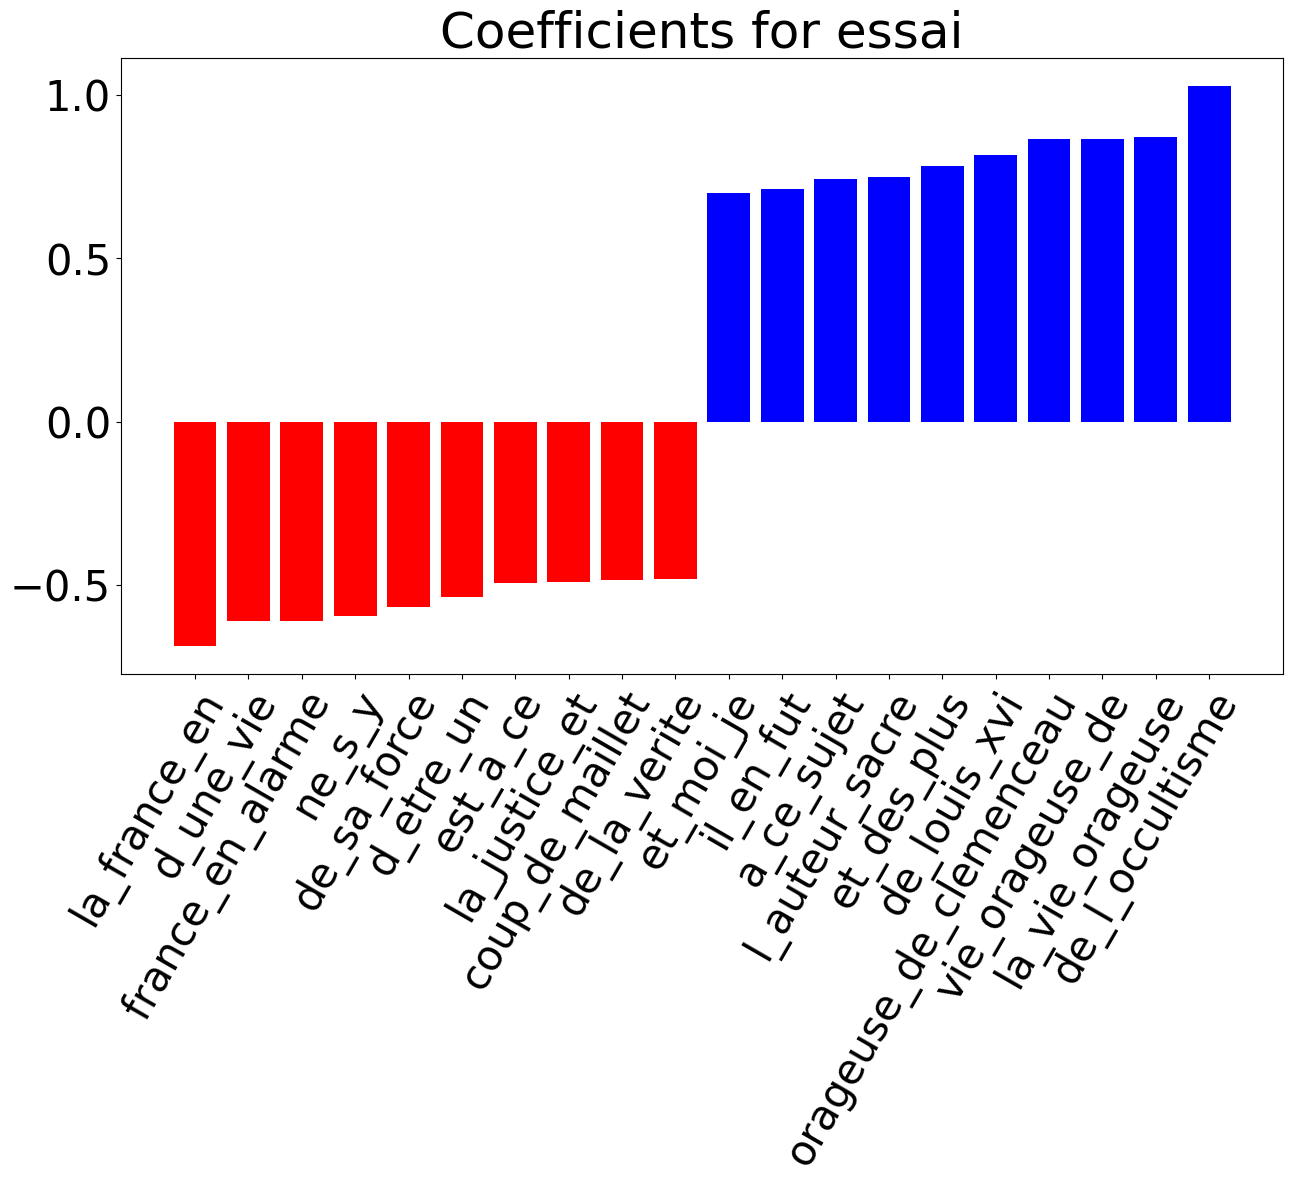
\includegraphics[width=0.70\textwidth]{img/coefs-corpus2-essai.png}
\caption{\textit{Diagramme à barres des coefficients de la classe essai du corpus 2}}
\label{'fig:coefs-corpus2-essai'}
\end{figure}

\begin{figure}[H]
\centering %
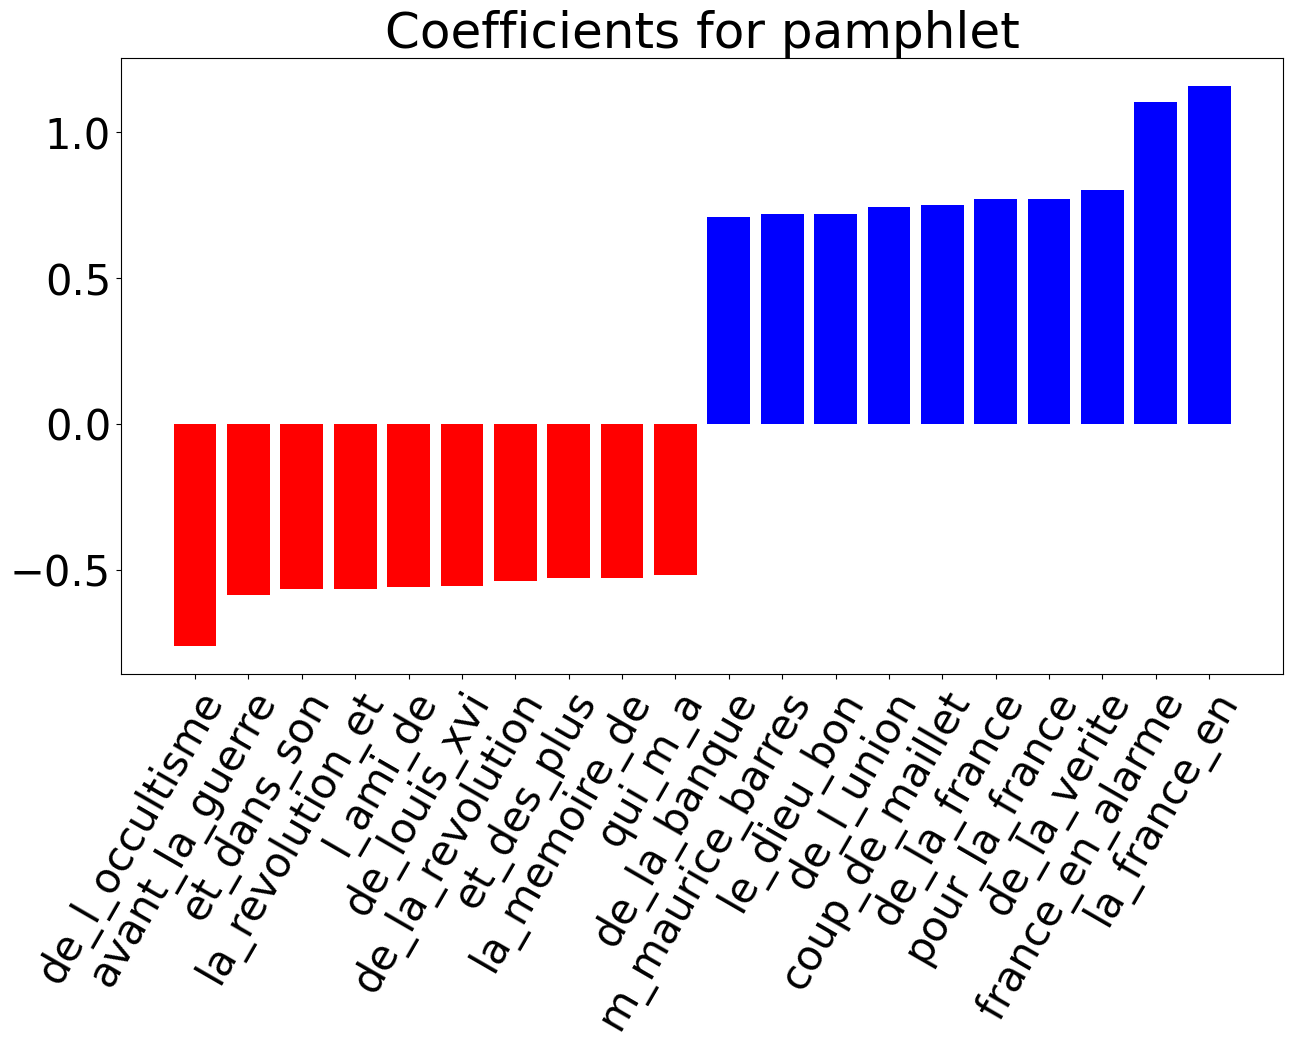
\includegraphics[width=0.70\textwidth]{img/coefs-corpus2-pamphlet.png}
\caption{\textit{Diagramme à barres des coefficients de la classe pamphlet du corpus 2}}
\label{'fig:coefs-corpus2-pamphlet'}
\end{figure}

Pour ce qui est de l'analyse des trigrammes reconnus comme pertinent par la SVM, nous nous permettons de remettre les accents là où il n'y a pas de doute sur leur présence, la SVM ne les prends pas en compte. Et nous unissons les trigrammes de mots qui forment une suite logique. Un problème majeur nous apparaît, une part conséquente des trigrammes sont liés aux titres des ouvrages tel que \enquote{\textit{appel au soldat}}, \enquote{\textit{au seuil de l'apocalypse}}, \enquote{\textit{le salut par les juifs}}, \enquote{\textit{le mendiant ingrat}}, \enquote{\textit{la vie orageuse de Clémençeau}}, \enquote{\textit{la france en alarme}} et quelques autres moins sur tel que \enquote{\textit{le scandale de la vérité}}. Cette apparition des titres d'ouvrages dans les trigrammes les plus représentatifs suppose des erreurs dans l'étape de la post-correction des OCR effectués par nous-même pour une part et des erreurs des versions numériques agrégées dans notre corpus pour une autre part. Ayant éludé ces trigrammes problématiques, nous obtenons quelques éléments sensés pour la classe roman  comme des éléments descriptifs \enquote{\textit{d'un air}}, \enquote{\textit{d'un ton}} et \enquote{\textit{d'une voix}} ainsi que deux trigrammes associés aux personnages \enquote{\textit{de son ami}} et \enquote{\textit{ce jeune homme}}. La classe mémoire mis à part le trigramme \enquote{\textit{de mes livres}} et la classe essai mis à part \enquote{\textit{et moi je}} ne sont pas parlants. La classe article met en lumière plusieurs occurrences de a conjonction \enquote{\textit{et}}. Enfin la classe pamphlet est composé de trigramme plus thématique tel que \enquote{\textit{de la france}} et \enquote{\textit{pour la france}}, \enquote{\textit{le dieu bon}} et \enquote{\textit{coup de maillet}}. On voit un certain lien avec la classe pamphlet du premier corpus ou un lexique du patriotisme frnaçais et de la religiosité poignent légèrement.
L'extraction de ces trigrammes par la SVM montre pour nous un intérêt analytique plus faible du fait de la présence de nom d'ouvrage en leur sein.
Enfin la \textit{table \ref{'tab:matriceconfusioncorpus2'}} montre que les classes de l'essai et du pamphlet sont assez perméables l'une de l'autre. Ces erreurs de prédiction peuvent montrer une plus proche proximité entre ces deux classes. Les erreurs de prédiction des classes vers la classe roman est assez homogène, c'est plus probablement le signal autorial qui doit causer ces erreurs.

\section{Conclusion}

Cette recherche de classification des genres permet de montrer que les textes pamphlétaires sont distinguables des genres narratifs du roman, de la nouvelle et des mémoire et biographie. Néanmoins, pour ce qui est de la distinction entre les articles et les essais vis-à-vis du pamphlet les dissimilitudes sont moins marquées. Cela tient de la proximité formelle des ces groupes. À titre d'ouverture et d'approfondissement, nous aurions aimé déployer les mêmes méthodes avec une approche de stylométrie roulante pour identifier plus clairement, depuis la classe pamphlet, les échantillons qui seraient identifiés comme similaire à l'essai, à l'article ou à la narration, ce qui permettrait d'approfondir les spécificités du pamphlet dans les échantillons de pamphlets dissimilaires de ces trois classes. 
Après avoir appliqué un outil d'analyse supervisé où la SVM recherche ce qui est commun à nos classes comme trait pertinent, nous souhaitons maintenant effectuer une analyse non-supervisé des deux mêmes corpus pour comprendre ce qui automatiquement rapprochent nos textes.

\chapter{Approche non-supervisé}

\section{La recherche de similarité générique non-supervisée}

L'analyse non-supervisé des données textuelles est un large pan de la textométrie et de la stylométrie. Le gain qu'apporte cette approche dans notre méthodologie est de caractériser les rapprochements et similitudes de nos textes sans présupposés sur leur appartenance à une classe. Depuis une même représentation vectorielle de nos corpus, nous cherchons à observer les rapprochements automatiques de nos textes par similitudes. La majorité de ces approches assurent des regroupements par auteurs, le signal autorial dans des genres issus de même champs génériques sont souvent plus fort que le style collectif d'un genre. Néanmoins nous souhaitons observer ce qui automatiquement rapproche nos textes et jouer sur différents paramètres pour au maximum faire émerger le style collectif du pamphlet. Pour nous prémunir d'un biais de comparaison du pamphlet d'un groupe d'auteurs restreint (13 pamphlétaires) face à une grande diversité d'écrivains d'autre genre (le corpus ANR Chapitres, Corpus 1), nous effectuerons une même analyse non-supervisé sur l'ensemble des textes de nos écrivains pamphlétaires (Corpus 2). 
Nous produirons deux chaînes de traitement distinctes, une classification ascendante hiérarchique et une analyse en composantes principales depuis une représentation matricielle de nos corpus ou (\textit{bag-of-words}). 
\par
Le concept de \textit{Bag-of-words}, ou sac de mots permet d'obtenir une représentation vectorielle de nos données textuelles. C'est une représentation simplifiée d'un document texte où l'ordre des mots est ignoré et seule la fréquence d'apparition des mots est prise en compte. Dans cette représentation chaque dimension est un mot unique et la valeur de celle-ci est sa fréquence dans un document donné. Nous parlons de mots, mais cela est vrai pour l'ensemble des \textit{features} que nous pourrions souhaiter extraire depuis les n-grams de caractères jusqu'à des n-grams de mots et bien d'autres encore. Cette seconde approche pour analyser nos données textuelles reprend les bases de l'extraction de \textit{features} de Superstyl que nous implémentons cette fois-ci nous même dans un soucis de contrôle fin des paramètres qui ajustent cette extraction. Notre implémentation permet de choisir le type de \textit{features} à extraire, mots, lemmes ou parti de discours ainsi que le nombre de n-grams ou la fenêtre de \textit{features} à sélectionner comme (1,3) ou (3,3). Les n-grams de (1,3) permettent de constituer une liste de l'ensemble des suites de gram (ou \textit{features}) de longueur 1 jusqu'à 3 par exemple.
La chaîne de traitement que nous mettons en place applique un calcul de fréquence, une normalisation L2 et une standardisation de nos \textit{features} pour obtenir notre représentation vectorielle.
Nous appliquons un calcul de fréquence brute à l'échelle des documents, un processus de normalisation correspondant à une mise à l'échelle des vecteurs de données pour qu'ils aient une certaine propriété, comme une longueur unitaire. Dans ce contexte, la normalisation L2 est utilisée, ce qui signifie que les vecteurs sont ajustés de manière à avoir une longueur euclidienne de 1. La mise à l'échelle standard implique de mettre à l'échelle les données de manière à ce qu'elles aient une moyenne nulle et un écart-type unitaire. Cependant, dans notre traitement, la mise à l'échelle standard est effectuée sans centrer les données autour de zéro car nous avons de nombreuses données creuses.


\section{Méthode choisie}

Nous appliquerons sur chacun des deux corpus définis précédemment pour la SVM notre propre chaîne de traitement. Nous n'effectuons pas d'échantillonnements par soucis de lisibilité des visualisations. Un échantillonement à rendrait le nombre de document à visualiser hors-norme. Nous appliquons un traitement unigram de mots non lemmatisé. Nous avons tenté avec des bigrammes et trigrammes de mots les mêmes analyses, le résultat ne différait peu. D manière itérative nous supprimons les \textit{features} en fonction d'un seuil où les \textit{features} non nulle doivent en être supérieurs. Cette étape de sélection de \textit{features} permet de réduire les variables aberrantes tel que les erreurs d'OCR ou autres \textit{hapax} que nous avons rencontrés au chapitre précédent sur le second corpus mais aussi cela permet de focaliser notre attention sur les valeurs mieux distribuées et potentiellement plus représentative de fait stylistique partagé. Le choix du seuil dépend des données et permet un aller-retour itératifs entre le seuil et les visualisations.
\par
Nous analyserons le fruit de cette matrice de sac de mots par un clustering ascendant hiérarchique et une analyse des Composantes Principales. Par soucis de visibilité nous produisons notre analyse sur des paires de 

\subsection{Clustering Ascendant Hiérarchique}

Le Clustering Ascendant Hiérarchique, abrégé en CAH, appartient à la catégorie des méthodes non supervisées, ce qui signifie qu'il est utilisé pour explorer et regrouper des données sans l'aide de variables cibles prédéfinies comme c'était le cas pour la SVM. Le CAH est particulièrement précieux lorsque l'on cherche à découvrir des structures intrinsèques, des similitudes et des dissimilarités au sein de données complexes et multidimensionnelles, c'est le cas pour nos données textuelles.
Le principe fondamental du CAH est de créer une hiérarchie de regroupements progressivement plus larges en fusionnant itérativement des éléments individuels ou des groupes de données similaires. À chaque étape, le CAH mesure la proximité ou la distance entre les données et combine les éléments les plus proches les uns des autres pour former des groupes de plus en plus vastes. Ce processus de fusion continue jusqu'à ce que toutes les données soient regroupées en un seul ensemble ou selon un critère prédéfini.
La première étape de la fonction implique le calcul de la distance entre les vecteurs représentant les documents dans l'espace des termes. Il existe plusieurs métriques pour définir la distance entre des données textuelles, nous choisissons la distance cosinus. Cette mesure de distance est choisie pour évaluer la similitude entre les documents en prenant en compte les angles entre leurs vecteurs, plutôt que les distances euclidiennes. La matrice de distance ainsi obtenue capture les dissimilarités entre les documents, où des valeurs plus élevées indiquent une dissimilitude plus importante.
À l'aide de la matrice de distance, l'algorithme d'agrégation hiérarchique avec méthode de Ward est employé pour former des groupes de documents en fonction de leurs similitudes. Cette approche construit progressivement une structure de regroupement en fusionnant les groupes les plus proches, en minimisant la variance intra-groupe. Nous générons ensuite une visualisation sous forme de dendrogramme, un diagramme arborescent utilisé pour représenter les regroupements hiérarchiques. Chaque feuille du dendrogramme correspond à un document du corpus. La coloration des branches du dendrogramme est déterminée par le seuil de couleur spécifié. Cette visualisation contrairement à d'autres permet de voir l'ensemble des différentes hiérarchies de cluster.

\subsection{Analyse en Composantes principales}

L'Analyse en Composantes Principales (ACP) est une technique de réduction de la dimensionnalité qui est couramment utilisée en statistiques et en apprentissage automatique pour explorer et analyser des données multidimensionnelles. Son objectif principal est de réduire la complexité d'un ensemble de données en projetant ces données dans un nouvel espace de plus petite dimension tout en conservant autant d'informations que possible. En d'autres termes, elle permet de trouver les combinaisons linéaires des variables d'origine (dans ce cas, les mots dans une matrice Bag-of-Words) qui expliquent le maximum de variabilité dans les données. Cette méthode consiste donc à transformer des variables corrélées en nouvelles variables dé-corrélées entre elles, ce qui est appelé les composantes principales.\par
L'ACP tire son origine du mathématicien Karl Pearson qui la développa au début du XX\ieme siècle. Ce sont ses travaux sur la régression qui le même à traiter des corrélations entre variables non pas pour expliquer une variable à partir des autres mais pour résumer et expliquer l'information contenue dans celles-ci. La formalisation des analyses factorielles dont l'ACP fait partie est déployé par Harold Hotelling, d'ailleurs le terme de transformation de Hotelling est utilisable pour parler de l'ACP. 
Cette capacité à réduire le nombre de dimension et à expliquer une matrice multivariée comme avec notre matrice de fréquences de \textit{features} de un gramme de mot est un atout pour l'explicabilité d'une classification des données.


\section{Résultats et analyses}

\subsection{Sortie du Corpus 1}

Nous présentons donc 3 paires de visualisations associées aux couples pamphlet-roman, pamphlet-mémoire et bio. et pamphlet-nouvelle. Les visualisation en dendrogramme sont accompagnées de trois niveau de légende correspondant à la qualification des textes en genre, auteur et titre, ce choix bien qu'alourdissant la visualisation apporte une meilleure visibilité. Le seuillage pour la colorisation des différentes branches du dendrogramme est fixé arbitrairement. 
La visualisation de l'ACP est fait en graphique bidimensionnel dont nous avons agrémenté la représentation des textes par des couleurs distinguant les genres et les motifs des points pour distinguer les auteurs. Nous omettons la légende des auteurs étant donné que le nom des textes suffit aisément à retrouver ceux-ci, l'intérêt de pouvoir rapidement évaluer l'appartenance d'un texte à un auteur par le choix des motifs de points permet de voir l'agglomération ou non de ceux-ci dans l'espace.

\par
Pour le \textit{dendrogramme \ref{'fig:dendogram-corpus-mix-PamRoman'}} du sous corpus pamphlet roman, nous constatons que la division par genre est fonctionnel sauf pour sept textes pamphlets de Léo Taxil, Laurent Thailade, Jules Vallès et Georges Darien. Nous observons néanmoins que les principaux groupes sont constitués avant tout par le signal autorial. 
Le \textit{graphique de l'ACP \ref{'fig:ACP-corpus-mix-PamRoman'}} quand à lui montre bien deux ensembles que nous soulignons nous même par l'emploi de couleurs distinctes par genre. Les différents motifs de points soulignent la distinction entre auteurs. Nous observons donc des regroupement par auteurs au sein de la division par genre. Le groupe de pamphlet paraît néanmoins très dispersé en opposition avec le groupe de roman. Cette disparité spatiale montre une certaine hétérogénéité des textes pamphlétaires. Nous retrouvons les mêmes cas ambiguës des pamphlets précédents aux plus près du groupe de roman tel que \textit{Les enfants du peuple} de Jules Vallès, \textit{Au pays du Mufle}, \textit{La Noire Idole}, \textit{Les Kalendes et les Ides} et \textit{À travers les Grouins} de Laurent Tailhade, \textit{Les Vrais Sous-Offs} de Darien et la \textit{Lanterne d'un suspendu} de Léo Taxil. Ces textes semblent être soit des cas limites à la frontières de deux genres soit une mauvaise attribution préalable de notre part nous reviendrons sur cela à la fin de cette partie.

\begin{figure}
\centering %
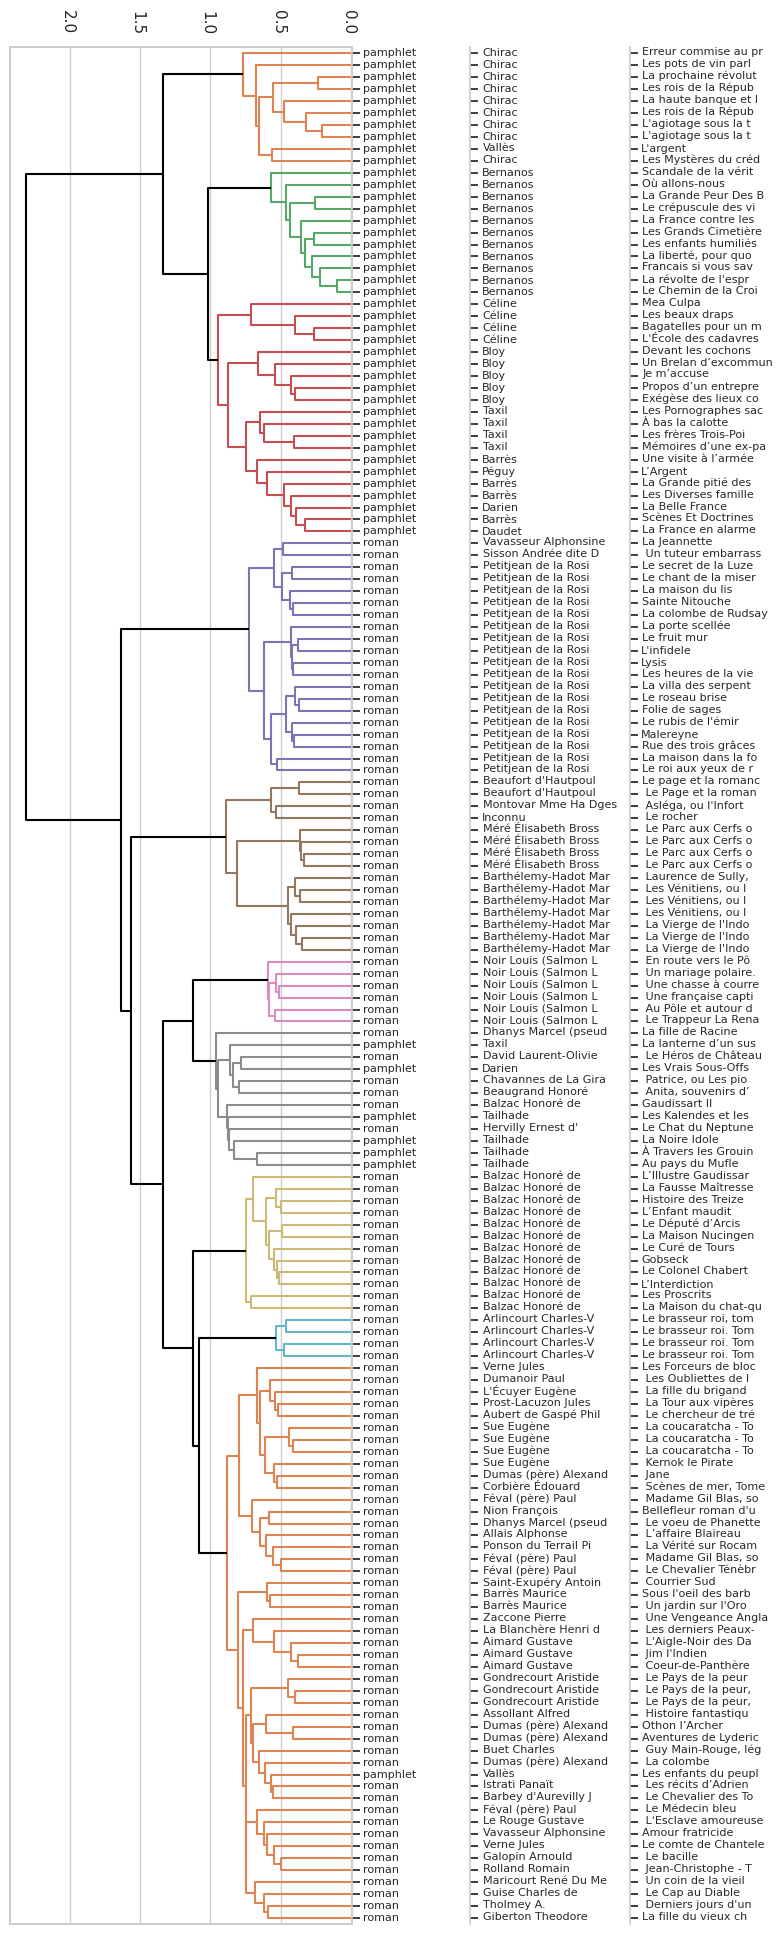
\includegraphics[width=0.60\textwidth]{img/dendogram-corpus-mix-PamRoman.png}
\caption{Dendrogramme de classification ascendante hiérarchique, Corpus 1, Genres pamphlet-roman, 1 n-gram de mot, 7192 / 107397 features, 25 non nulle}
\label{'fig:dendogram-corpus-mix-PamRoman'}
\end{figure}

\begin{figure}[H]
\centering %
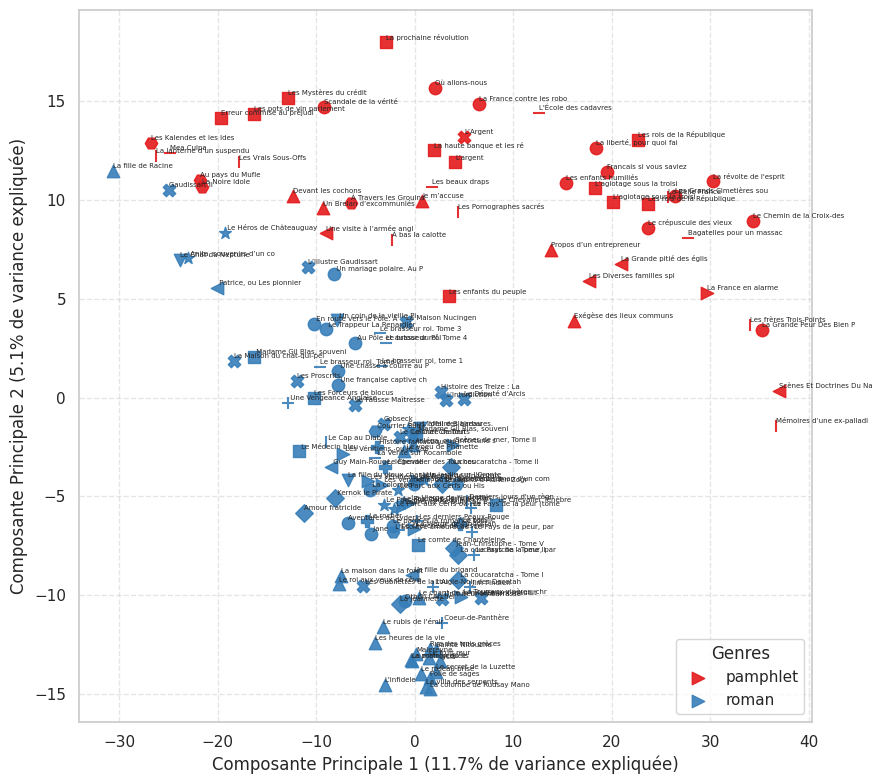
\includegraphics[width=1\textwidth]{img/ACP-corpus-mix-PamRoman.png}
\caption{Analyse en composantes principales, Corpus 1 Genres pamphlet-roman}
\label{'fig:ACP-corpus-mix-PamRoman'}
\end{figure}

Pour le sous corpus formant la paire pamphlet-mémoire et biographie, nous observons exactement les mêmes textes que précédemment être exclue de l'ensemble constitué de pamphlet. Trois mémoires et bio. sont elles-mêmes inclus dans l'ensemble de pamphlet. Les \textit{Lettres de Bayreuth} de Charles Henri Tardieu sont un cas ambigu, la forme même du recueil de lettres avec un style mélangé journalistique et essayistique et le ton très incarné assez proche de la figure des pamphlétaires tend à montrer les limites d'une approche statistique. Voici un bref extrait assez représentatif de ce ton :\\

\par\textit{ Bayreuth, 14 août 1876, matin 
 Vous me demandez la vérité vraie, c'est fort bien, mais la mienne, ma vérité à moi, ne sera peut-être pas vraie pour vous, et la vôtre pourrait bien être la fausseté même pour les quinze cents personnes qui ont acclamé hier soir l'auteur de l'Anneau du Nibelung. Il y a vingt vérités vraies, il y en a cent, il y en a mille en art, comme en religion et en politique. Je renonce à chercher la plus vraie de toutes, la seule vraie, la vérité des vérités. Tout ce que vous pouvez exiger de votre correspondant, c'est la sincérité. Permettez donc que je vous donne franchement et tout bêtement mon sentiment.} Lettres de Bayreuth, Charles Henri Tardieu.

Cela se rapproche de ce qu'à pu écrire Léon Bloy dans ses chroniques du Chat Noir rassemblé dans \textit{Propos d'un entrepreneur de démolitions} Ce texte issu de l'ARN Chapitres est donc un cas limite en soi. Le second et troisième cas spéciaux sont les deux tomes du \textit{Voyage d'un jeune grec} d'Hippolyte Mazier du Heaume. Ce texte semble aussi être un cas limite, le thème est artistique mais le ton est virulent.
La visualisation de l'ACP montre une grande dispersion des pamphlets face à une certaine homogénéité du groupe de mémoire, excepté une porosité entre les cas limite de pamphlet comme précédemment, les cas de mémoires et biographies spécieux auquel nous pouvons ajouter \textit{Aden Arabie} de Paul Nizan, nous avions évoqués ce texte qui fut dans le cas de la SVM aussi un cas limite que nous retrouvons ici.

\begin{figure}[H]
\centering %
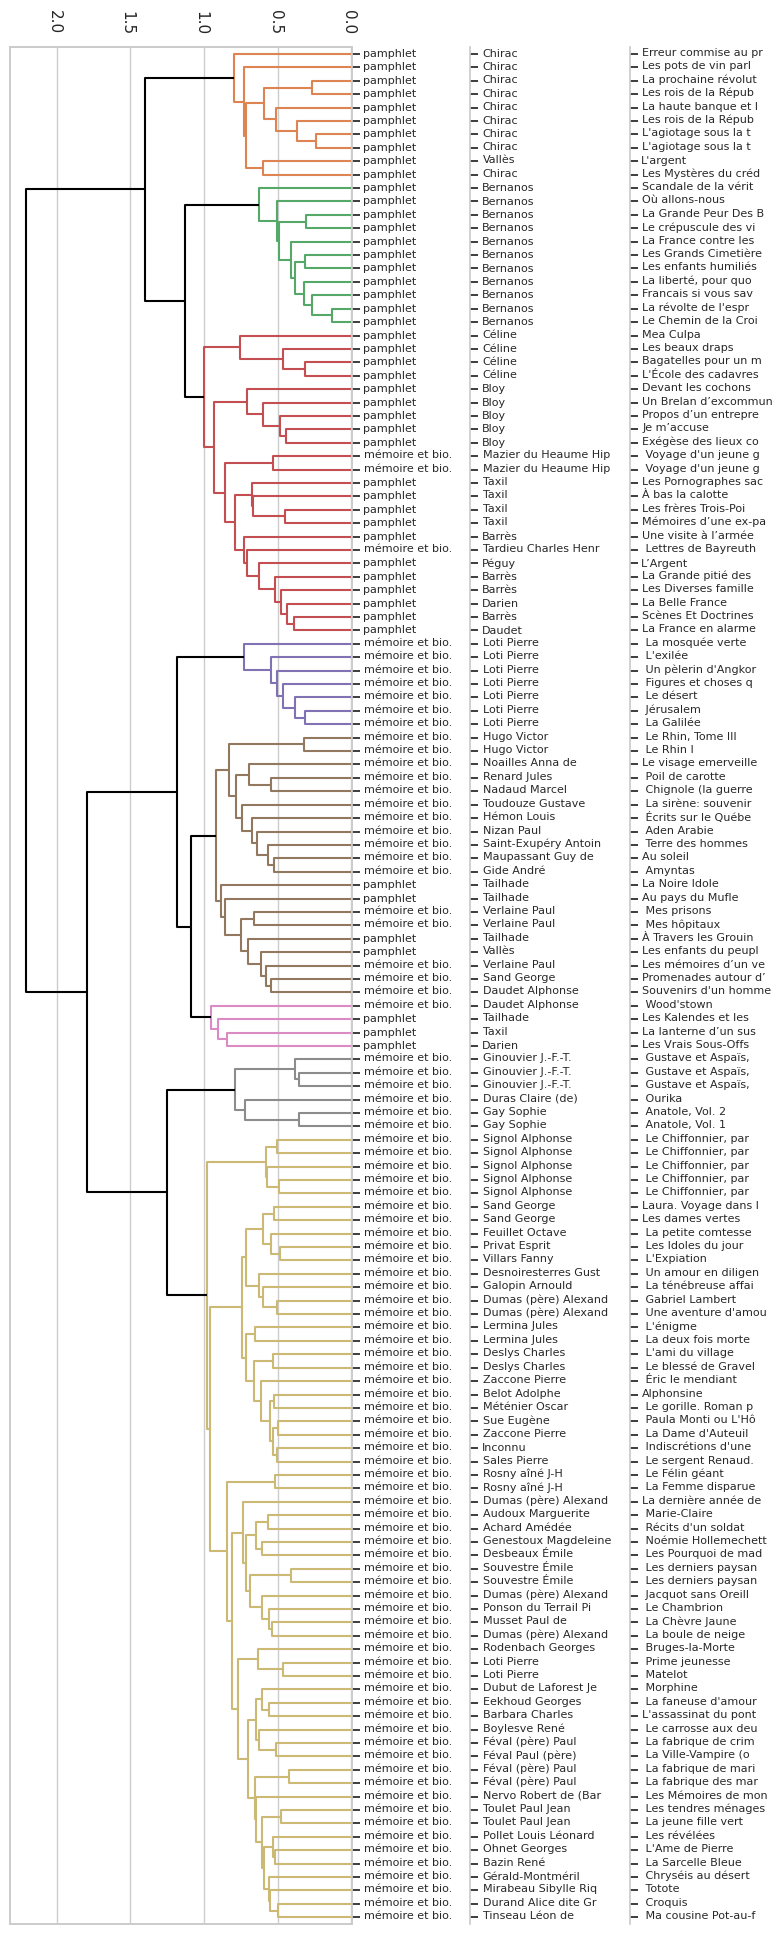
\includegraphics[width=0.60\textwidth]{img/dendogram-corpus-mix-PamMem.png }
\caption{Dendrogramme de classification ascendante hiérarchique, Corpus 1, Genres pamphlet-mémoire et biographie, 1 n-gram de mot, 8833 / 110741 \textit{features}, 25 non nulle}
\label{'fig:dendogram-corpus-mix-PamMem'}
\end{figure}

\begin{figure}[H]
\centering %
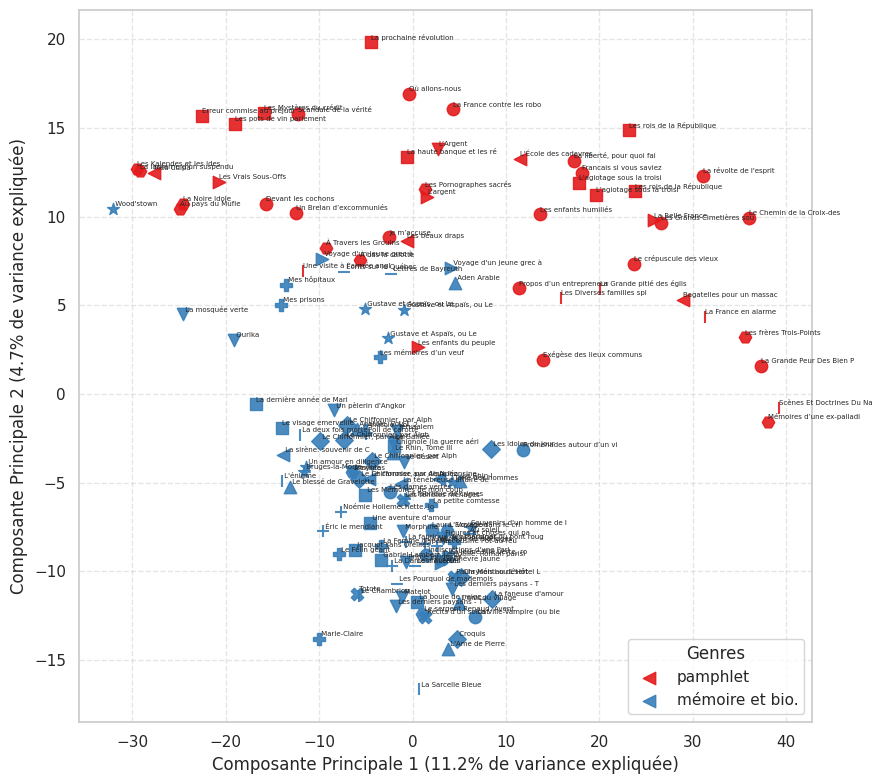
\includegraphics[width=1\textwidth]{img/ACP-corpus-mix-PamMem.png}
\caption{Analyse en composantes principales, Corpus 1, Genres pamphlet-mémoire et biographie}
\label{'fig:ACP-corpus-mix-PamMem'}
\end{figure}


Pour cette troisième paire pamphlet-nouvelle nous constatons que les mêmes textes classés pamphlet par nos soins qui se trouvaient placés hors des branches pamphlétaires pour les dendrogrammes précédent se retrouvent hors de la branche pamphlétaire du \textit{dendrogramme \ref{'fig:dendogram-corpus-mix-PamNouvelle'}} hormis \textit{Les enfants du peuple} de Jules Vallès qui cette fois-ci fait parti de cette branche pamphlétaire, cela permet de remettre en équilibre sa dimension de cas limite. Pour le reste des textes spécieux pamphlets, nous pouvons encore constater leur positionnement spatial comme en marge des deux ensembles.

\begin{figure}[H]
\centering %
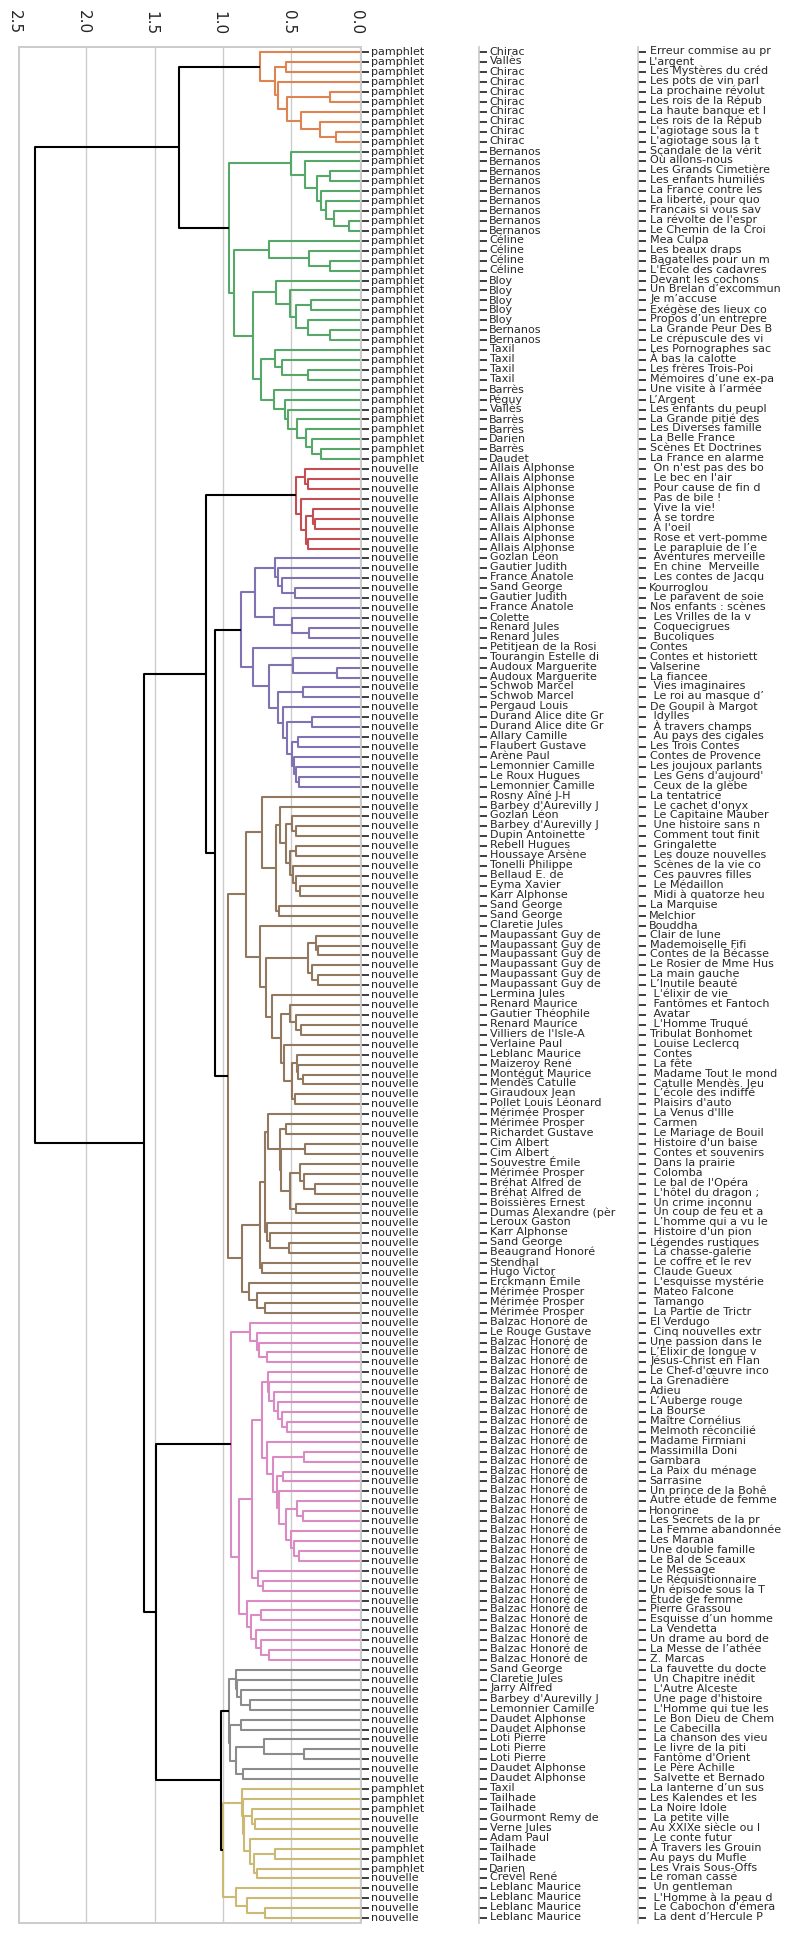
\includegraphics[width=0.60\textwidth]{img/dendogram-corpus-mix-PamNouvelle.png}
\caption{Dendrogramme de classification ascendante hiérarchique, Corpus 1, Genres pamphlet-nouvelle, 1 n-gram de mot, 5700 / 113137 \textit{features}, 40 non nulle}
\label{'fig:dendogram-corpus-mix-PamNouvelle'}
\end{figure}


\begin{figure}[H]
\centering %
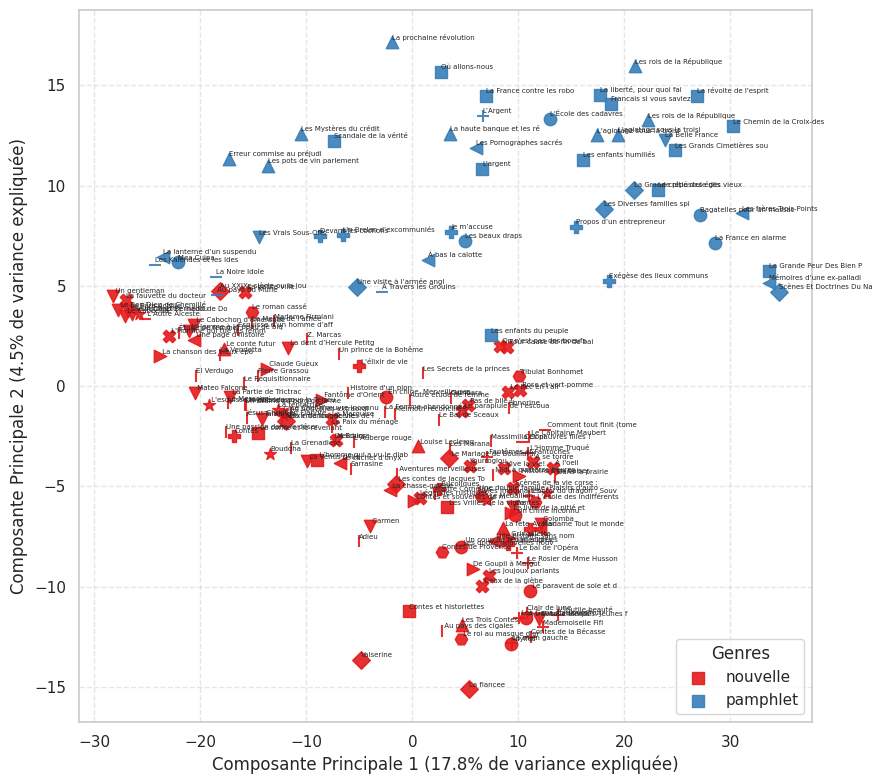
\includegraphics[width=1\textwidth]{img/ACP-corpus-mix-PamNouvelle.png}
\caption{Analyse en composantes principales, Corpus 1 Genres pamphlet-nouvelle}
\label{'fig:ACP-corpus-mix-PamNouvelle'}
\end{figure}

Ces différentes analyses tendent à montrer une nette distinction entre le champ générique de la narration représenté par les mémoires et biographies, les romans, les nouvelles et les pamphlets.
La visualisation de la classification ascendante hiérarchique en dendrogramme nous laisse à penser que cette distinction est franche et que le pamphlet forme un ensemble aussi cohérent que les différents genres mis en comparaison. Néanmoins la visualisation de l'analyse en composantes principales nous montre une dispersion plus grande du groupe de pamphlet qui est bien moins homogène dans sa répartition spatiale que pour les genres d'où nous le comparons.

\subsection{Sortie du Corpus 2}

Nous appliquons donc les mêmes méthodes sur ce second corpus uniquement composés des textes que nous avons agrégés des auteurs pamphlétaires. Cette seconde salve d'analyse à pour but d'observer la force du signal générique face à celle du signal autorial. Étant donné que l'ensemble des textes se divise en une poignée d'auteurs, les similarités des textes risquent fort de se faire par auteurs. Ayant ce biais à l'esprit nous savons que les visualisations en dendrogramme risquent d'être moins pertinentes car plus aptes à montrer un rapprochement par auteurs. Mais nous espérions que la visualisation de l'ACP puisse quand même apporter des regroupements génériques. Nos analyses sur le corpus précédent ont montré une claire frontière entre le champ générique de la narration et celui du pamphlet, ce que nous retrouverons ici malgré le bruitage du signal autorial. Ce qui nous intéresse plus particulièrement sont les comparaisons des pamphlets face aux essais et aux articles. En effet, ces trois genres partagent une proximité générique bien supérieur à ce que partagent, le pamphlet et le roman par exemple. 

\begin{figure}
\centering %
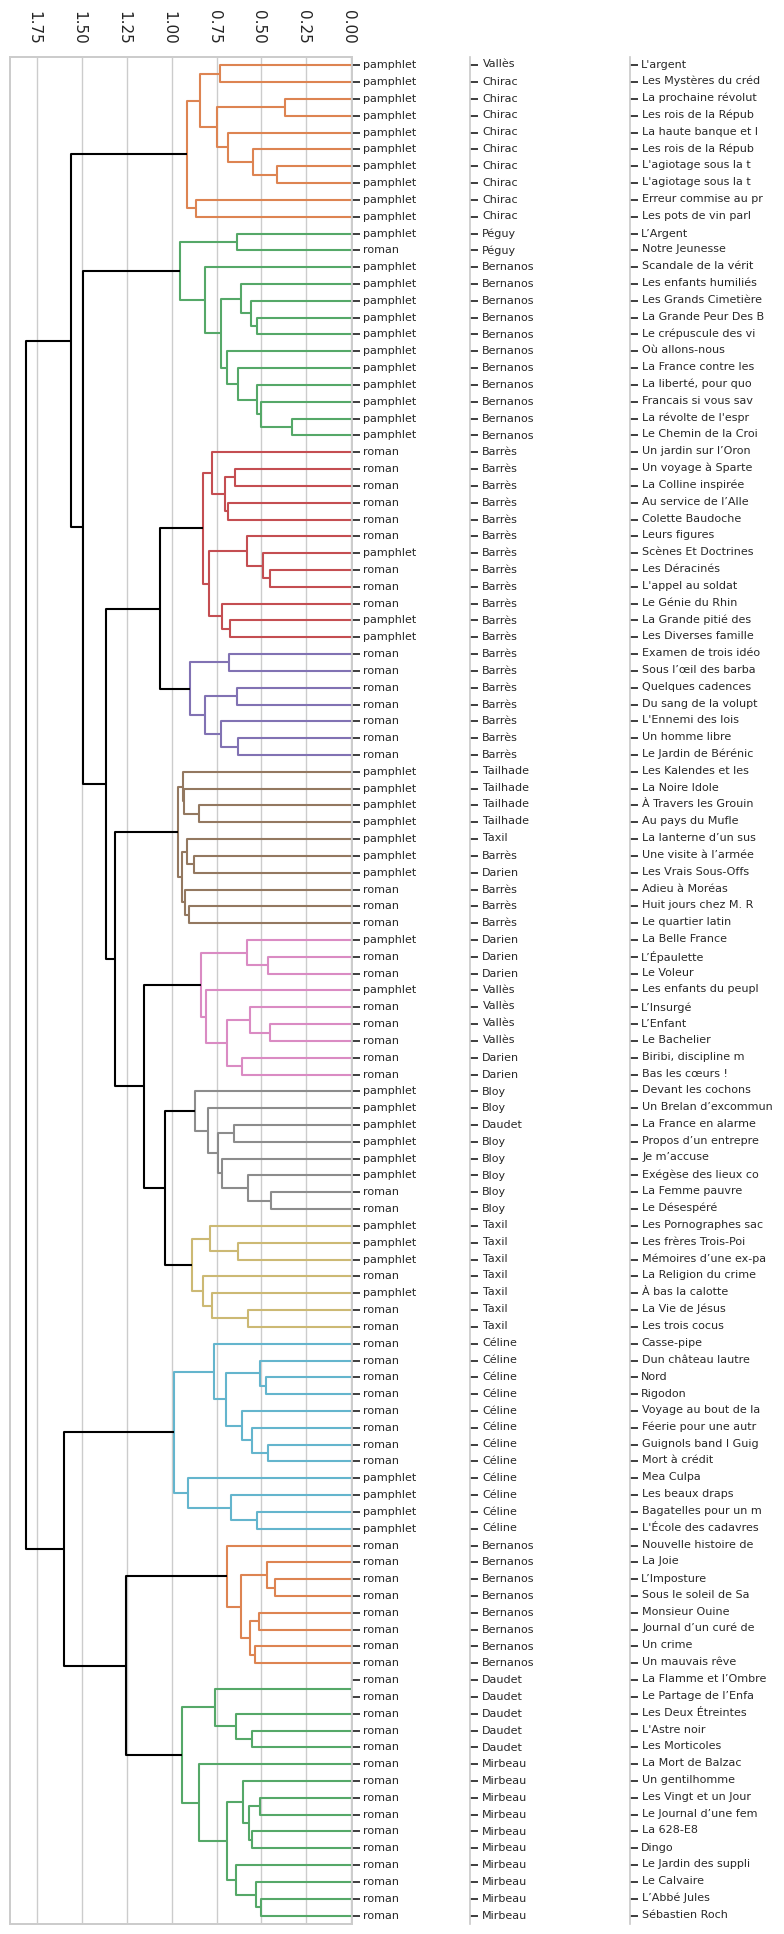
\includegraphics[width=0.6\textwidth]{img/dendogram-corpus-2-PamRoman.png}
\caption{Dendrogramme de classification ascendante hiérarchique, Corpus 2, Genres pamphlet-roman, 1 n-gram de mot, 22272 / 131547 \textit{features}, 25 non nulle}
\label{'fig:dendogram-corpus-2-PamRoman'}
\end{figure}

\begin{figure}[H]
\centering %
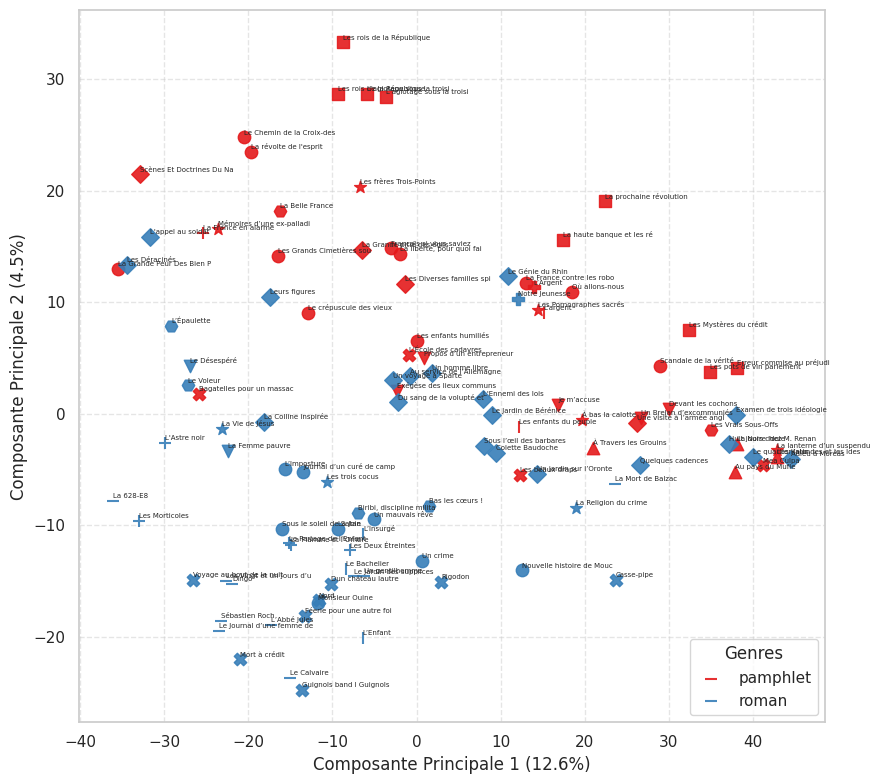
\includegraphics[width=1\textwidth]{img/ACP-corpus-2-PamRoman.png}
\caption{Analyse en composantes principales, Corpus 1 Genres pamphlet-roman}
\label{'fig:ACP-corpus-2-PamRoman'}
\end{figure}

Pour la comparaison du pamphlet et du roman, nous observons une plus grande difficulté à saisir la hiérarchisation des branches de la visualisation en dendrogramme. La formation des branches oscille entre une division par auteur et par genre. Par exemple pour les textes de Georges Bernanos, la division s'effectue par genre assez clairement, alors que pour Louis-Ferdinant Céline, c'est bien l'attribution autoriale qui prédomine. Les choix de la formation des branches suivant le clustering ascendant hiérarchique montre bien une incertitude sur la capacité à classer les textes en genre. L'exemple de la répartition fragmentée des textes de Jules Vallès entre signal autorial et générique renforce cet avis. Nous nous attendions à ce fort bruitage. Les cas de pamphlet spécieux du précédent corpus ne réapparaissent pas avec la même évidence, \textit{Les enfants du peuple} de Jules Vallès est associé au roman de ce même auteur avec une branche divergente là où la majorité des autres cas spécieux se retrouvent dans la même branche au coté de trois romans de Maurice Barrès. Nous pouvons soutenir que ces cas ambigus de pamphlets continuent de l'être dans ce corpus. Cette indisctinction entre classification générique ou autorial rend plus difficile une analyse complète.
Nous retrouvons cette oscillation dans la visualisation de l'analyse en composantes principales, où bien que de grande tendance de groupe émerge entre pamphlet et roman, ces deux ensemble n'ont pas de marges et même partage une union assez marquée. La proximité par auteur bien qu'évidente n'est pas aussi intuitive que nous le présentions. Les exemples de l'emplacement de \textit{Bagatelles pour un massacre} ou de l'ensemble des textes de Maurice Barrès réparti à la jonction des deux ensembles montrent une incapacité à établir clairement une distinction de genre par cette méthode sur ce corpus.

\par
La comparaison des mémoires et biographies face aux pamphlets, ainsi que des nouvelles faces aux pamphlets souffre d'une indigence de diversité d'auteurs. La majorité des mémoires et biographies sont écrites par Léon Bloy ce qui ne permet pas une réelle comparaison de genre, le biais induit est trop grand. Et le nombre de nouvelle est cinq fois moins grand que le nombre de pamphlet. Nous ne nous tardons pas sur ces cas biaisés, néanmoins les visualisations en \textit{dendrogramme \ref{'fig:dendogram-corpus-2-PamMem'}} et celle de \textit{l'ACP \ref{'fig:ACP-corpus-2-PamMem'}} de la comparaison des mémoires et biographies ainsi que le \textit{dendrogramme \ref{'fig:dendogram-corpus-2-PamNouvelle'}} et la visualisation de \textit{l'ACP \ref{'fig:ACP-corpus-2-PamNouvelle'}} sont accessibles depuis l'annexe.

\begin{figure}[H]
\centering %
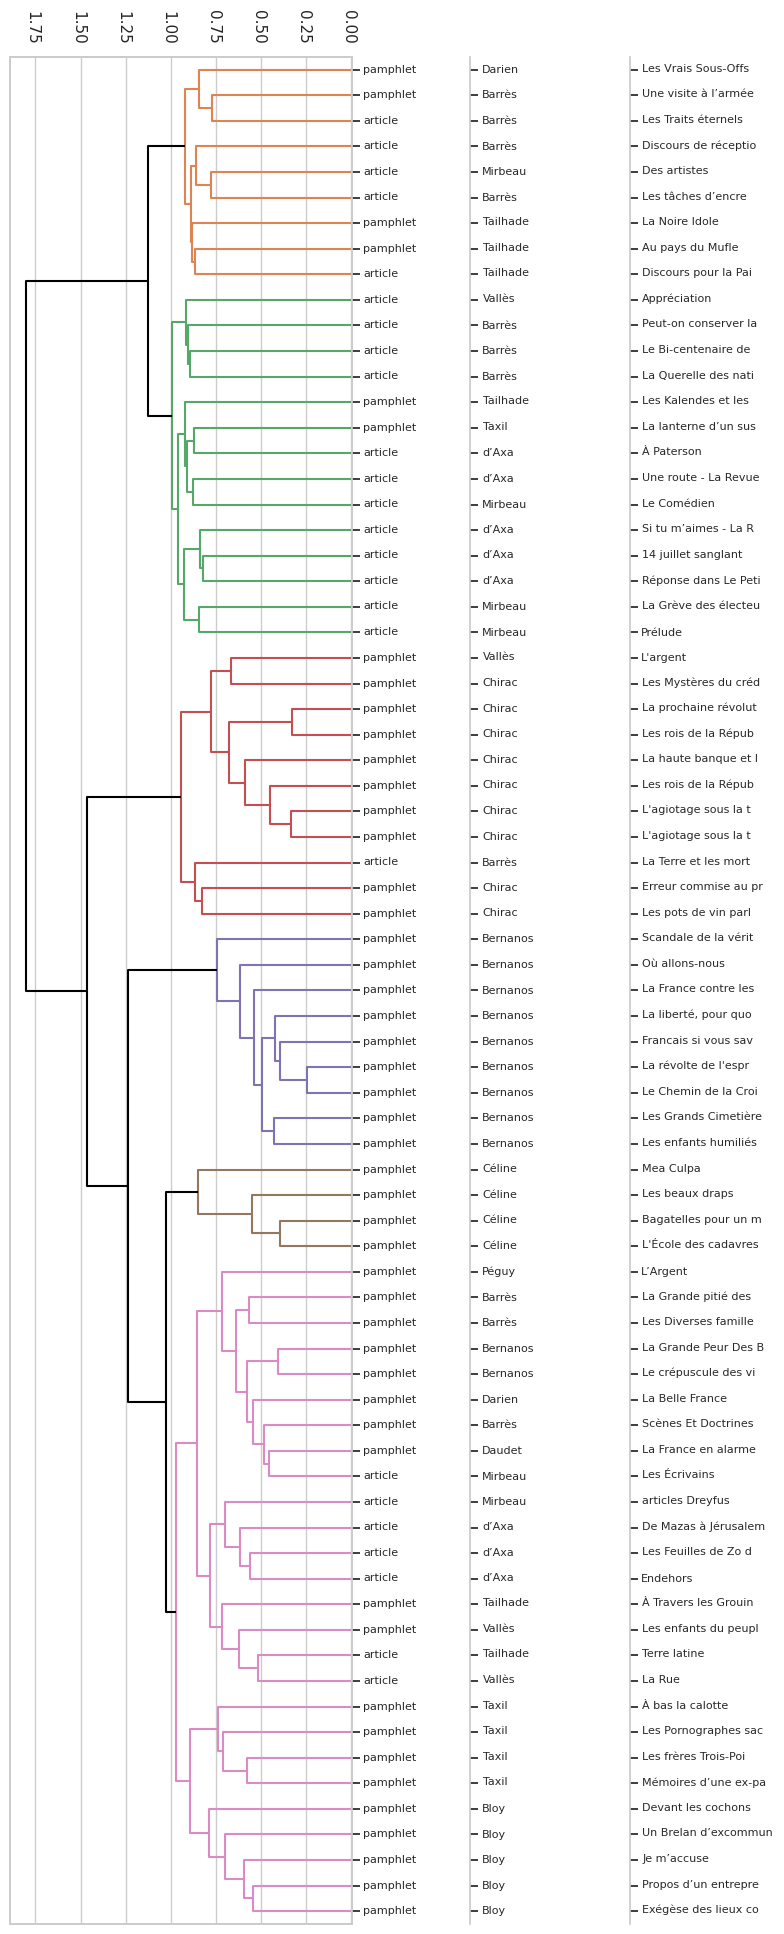
\includegraphics[width=0.60\textwidth]{img/dendogram-corpus-2-PamArticle.png}
\caption{Dendrogramme de classification ascendante hiérarchique, Corpus 2, Genres pamphlet-article, 1 n-gram de mot, 11650 / 92139 \textit{features}, 40 non nulle}
\label{'fig:dendogram-corpus-2-PamArticle'}
\end{figure}


\begin{figure}[H]
\centering %
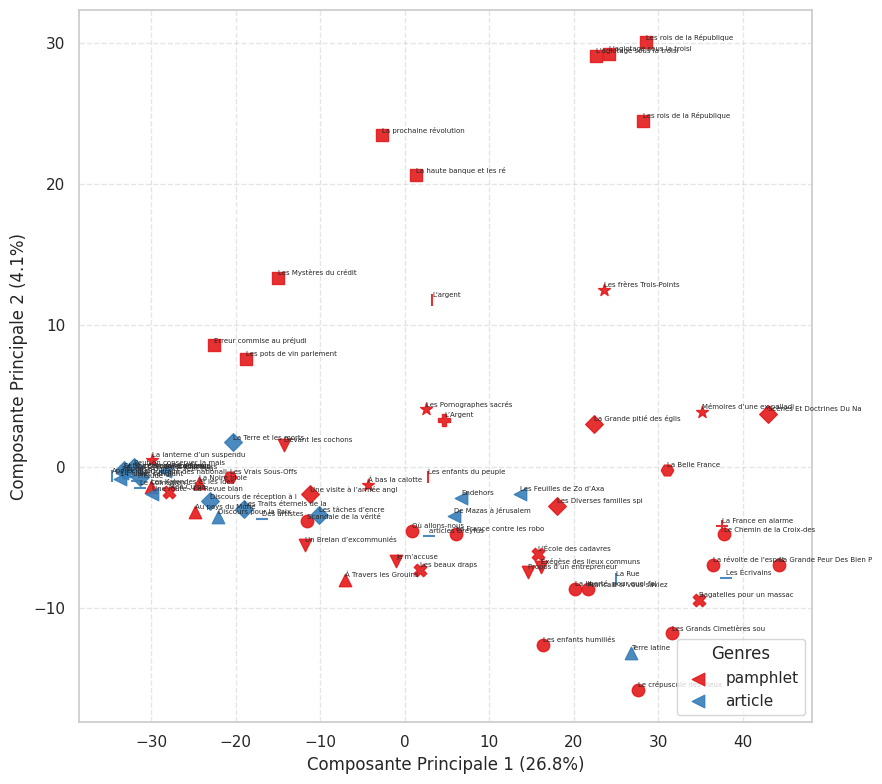
\includegraphics[width=1\textwidth]{img/ACP-corpus-2-PamArticle.png}
\caption{Analyse en composantes principales, Corpus 2 Genres pamphlet-article}
\label{'fig:ACP-corpus-2-PamArticle'}
\end{figure}

La comparaison des pamphlets et des articles rend compte d'une difficulté similaire de visualisation et d'interprétation des résultats. Sur le dendrogramme il semble y avoir des regroupements par genre en deux branches majoritairement pamphlet pour l'une et majoritairement article pour l'autre. Au sein de ces branches le regroupement par auteurs est le plus commun. Néanmoins sur les six textes qualifiés de pamphlet présent dans la branche article, nous retrouvons nos cas de pamphlets spécieux avec \textit{Les Vrais Sous-Offs}, \textit{La Noire Idole}, \textit{Les Kalendes et les Ides} et \textit{La Lanterne d'un suspendu} mais aussi \textit{Au pays du Mufle} qui était un cas ambigu pour la comparaison avec le roman.
Pour les cas des articles regroupés dans des branches contenant majoritairement des pamphlets, nous trouvons deux textes d'Octave Mirbeau, trois de Zo d'Axa, un de Laurent Tailhade et un de Jules Vallès. Il est intrigant de retrouver deux articles d'O. Mirbeau et de Z. d'Axa dans la branche pamphlet alors même qu'il y a des articles de ces mêmes auteurs dans la branche principale des articles. La force du signal autorial devrait à notre sens devoir les regrouper bien plus logiquement. En se tournant vers l'analyse en composantes principales nous constatons que les articles et les pamphlets semblent spatialement peu distinguables. Des regroupement par auteur s'observent dans la plupart des cas. Le groupe de pamphlet est assez dispersé notamment avec les textes d'Auguste Chirac. Nous constatons que les pamphlets spécieux, nos mêmes cas ambigus, sont les plus proches de la zone très agglomérée du groupe des articles. Et que les articles qui étaient regroupés dans la branche pamphlet du dendrogramme sont totalement excentré du groupe d'article de la visualisation de l'ACP. En laissant de coté le cas des pamphlets spécieux, nous pouvons donc affirmer que les unigrammes de mots supposent une proximité entre les pamphlets et les articles des mêmes auteurs de manière plus significatif qu'entre les pamphlets et les romans. À  ce stade nous ne pouvons pas interpréter les raisons de cette proximité avec nos analyses CAH et ACP mais cela se révèle à l'échelle des fréquences de mots.


\begin{figure}[H]
\centering %
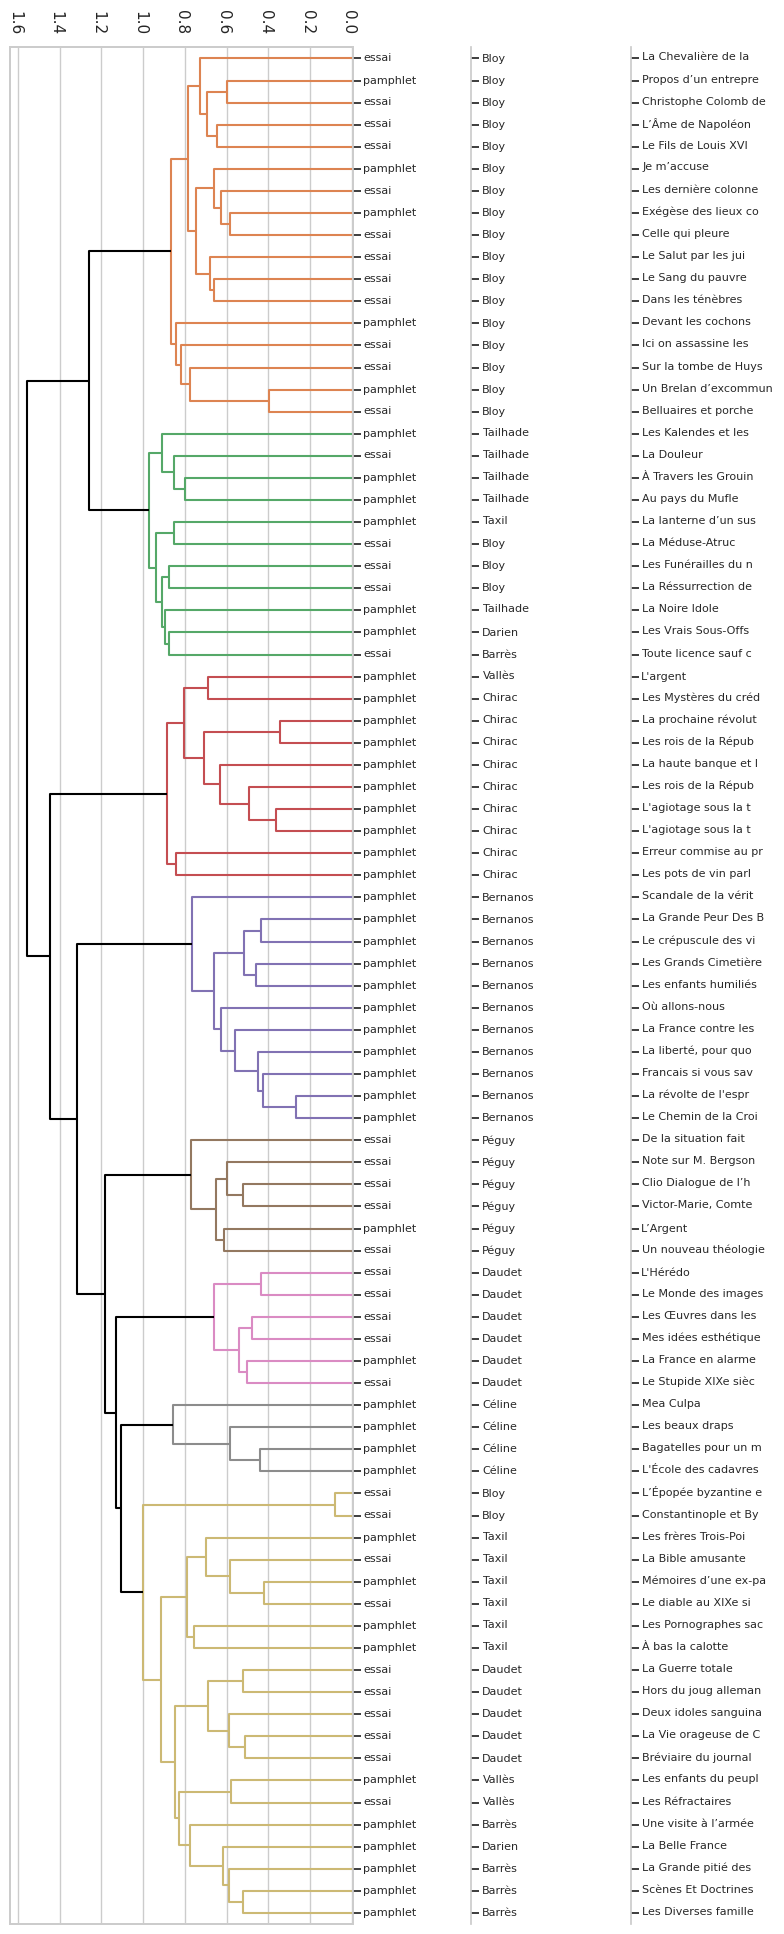
\includegraphics[width=0.60\textwidth]{img/dendogram-corpus-2-PamEssai.png}
\caption{Dendrogramme de classification ascendante hiérarchique, Corpus 2, Genres pamphlet-essai, 1 n-gram de mot, 15492 / 110867 \textit{features}, 40 non nulle}
\label{'fig:dendogram-corpus-2-PamEssai'}
\end{figure}


\begin{figure}[H]
\centering %
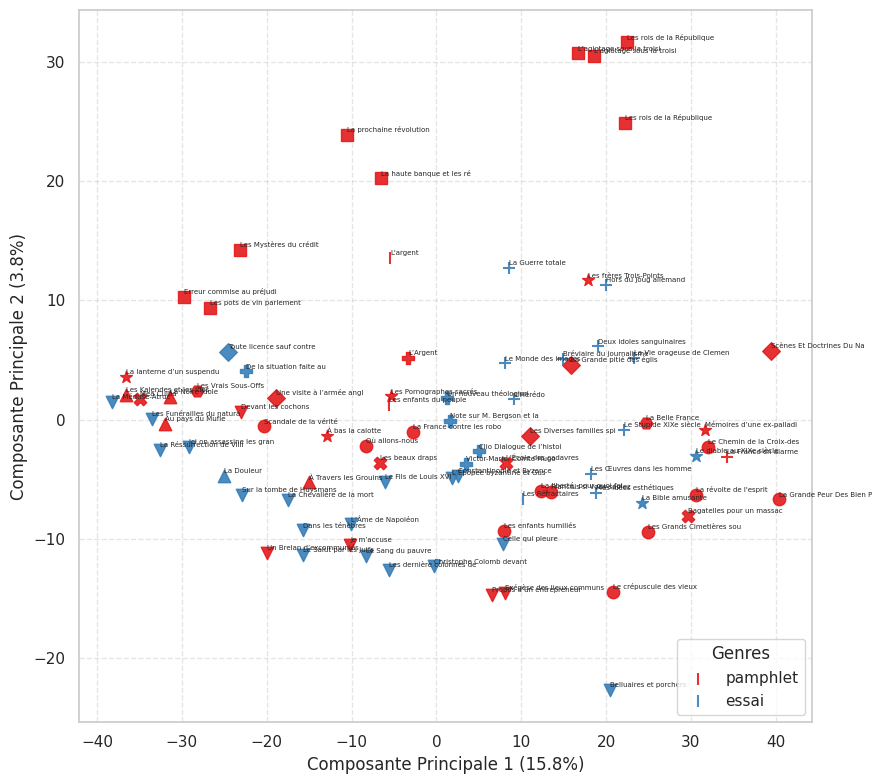
\includegraphics[width=1\textwidth]{img/ACP-corpus-2-PamEssai.png}
\caption{Analyse en composantes principales, Corpus 2 Genres pamphlet-essai}
\label{'fig:ACP-corpus-2-PamEssai'}
\end{figure}

La dernière comparaison entre pamphlet et essai est la plus intéressante pour cette étude. Marc Angenot, comme nous avons pu l'expliquer dans l'introduction, fait du pamphlet et de l'essai une appartenance commune aux discours enthymématique et doxologique. Cette appartenance suppose donc de pouvoir observer des faits de langues communs aux pamphlet et essai. Malgré cette grande proximité nous souhaitons pouvoir observer une divergence entre ces deux ensembles. Lorsque l'on se tourne vers cette dernière visualisation en dendrogramme, nous ne pouvons à première vu observer uniquement une ramification par auteur. Une branche comporte plus de pamphlet mais la distinction est ténu voir quasi nulle. Nos pamphlets spécieux se retrouvent tous dans une branche composée uniquement d'essais d'autres auteurs hormis un essai de Laurent Tailhade. La constance de la répartition de ces pamphlets spécieux souligne une dissemblance forte de ces textes avec le reste de l'ensemble de nos pamphlets. Nous pouvons souligner que certains essais de Léon Bloy, bien qu'une branche identifie la majorité de ces textes pamphlets et essais ensemble, se retrouvent dans des branches très éloignés, nous ne savons pas interpréter cet écart.
La visualisation de l'analyse en composantes principales, \textit{figure \ref{'fig:ACP-corpus-2-PamEssai'}}, ne nous permet pas de déceler une distinction entre le groupe de l'essai et celui du pamphlet, les deux étant indiscernables spatialement. Nous retrouvons encore les textes d'Auguste Chirac assez excentré de l'ensemble. Cette absence de distinction nous force à constater que l'analyse de la fréquence des unigrammes de mots ne sont pas une variable pertinente pour constater une distinction formelle entre les textes pamphlétaires et les essais de mêmes auteurs.

\section{Conclusion}

La méthode non-supervisée que nous avons mis en place avec une analyse en composantes principales et une classification ascendante hiérarchique ont chacune pu offrir un regard complémentaire l'un pour l'autre sur une même matrice de sac de mot d'unigramme. L'enjeu du choix d'analyser le premier corpus composé de textes pamphlétaires et d'autres genres appartenant au champ générique de la narration issu de l'ARN Chapitres a permis de montrer une nette distinction générique entre eux. Cela valide la pertinence de cette approche pour étudier les marques génériques par l'emploi des mots mêmes. L'application de cette méthode sur le second corpus devait servir plus spécifiquement à observer un même découpage générique malgré la présence bien plus forte du signal autorial, c'est-à-dire le rapprochement naturelle des textes par auteurs. Autant cela a pu fonctionner pour le roman, autant cela n'a pas été pertinent pour distinguer les articles et essais du pamphlet. Nous avons tenté d'augmenter le nombre de n-gram et le seuillage de suppression des n-grams peu fréquents sans succès. Nous n'avons pas reproduit ici le résultat de ces tentatives infructueuses sur des ngrams plus grands. Nous en concluons que la variable de sac de mots de n-grams n'est pas pertinent pour distinguer des textes d'un groupe d'auteurs restreints sur la focal générique lorsque ces genres partagent une très grande proximités entre eux tel le pamphlet et l'essai. Néanmoins sont ressortis de cette analyse des textes que nous avons qualifié de pamphlet alors qu'ils semblent être des cas limites ou spécieux, c'est à dire des textes qui tendent à diverger fortement de l'ensemble pamphlet du reste de nos analyses et visualisations. Ils mériteraient une analyse plus fine pour comprendre si seule des passages de ces textes permettent de les réintégrer pleinement dans l'ensemble pamphlet ou si il s'agit d'une mauvaise attribution de départ.


\part{Énonciation et motifs}

\chapter{L'Énonciation}

\section{Propos liminaires}

Après avoir procédé à différentes analyses assez traditionnelles (avec les approches complémentaires supervisées et non-supervisées) en humanités numériques pour défricher nos textes pamphlétaires et faire émerger ou plus simplement constater quantitativement certains rapprochement de nos pamphlets avec différents genres, nous souhaitons dans cette partie interroger directement des aspects distinctifs du genre pamphlétaire. Cela va se faire avec la présentation de deux analyses, l'une portant sur l'énonciation pamphlétaire, l'autre sur la recherche de motifs. L'énonciation pamphlétaire, déjà occultée par Marc Angenot dans son travail que nous citons toujours, \enquote{\textit{La parole pamphlétaire}}, déploie un discours précis sur la relation du locuteur-narrateur de l'allocutaire et de l'adversaire : le \enquote{je}, le \enquote{vous} qui forment un \enquote{nous} face à un \enquote{il}.  Nous analyserons cela en cherchant quantitativement à définir une spécificité du pamphlet dans son emploi des pronoms. La recherche de motifs génériques, inspirée du travail de Thierry Poibeau et al. sur le cliché amoureux \footcites{legallois_reperer_2016}, nous permettra de chercher des structures génériques au seins des phrases.


\section{Définition énonciation}

L'énonciation en stylistique et dans les principes de la pragmatique est d'un grand secours pour définir certaines spécificités du pamphlet comme genre littéraire. L'énoncé littéraire est pris comme moyen et résultat d'un acte de parole qui suppose plusieurs instances. Le pamphlet genre complexe partage plusieurs caractéristiques de l'énonciation avec d'autres genres comme le discours délibératif, l'essai polémique et l'article journalistique. De l'énonciation de l'essai polémique, le pamphlet est associé a l'ensemble du genre agonique (ou littérature de combat). Le pamphlet est surtout un discours agressif et violent, énonçant régulièrement l'image d'un contre-discours à réfuter et disqualifier. Cette disqualification propre à la polémique dans le cadre du pamphlet s'étend à la disqualification totale d'un adversaire car existe alors un scandale de la Vérité à révéler. Le pamphlet porte aussi un discours persuasif, l'énonciateur veut persuader le destinataire d'une vérité qu'il juge travesti, en ce sens il conserve certaine caractéristique du genre délibératif. Le pamphlétaire destine son discours à deux auditoires distincts, l'un étant un destinataire universel que l'on persuade et l'autre étant un adversaire que l'on disqualifie. Cette double destination du pamphlet complexifie le schéma de l'énonciation qui distingue le genre de ses proches parents: la polémique et la satire. Autrement dit le discours instaure une opposition entre deux adversaires le pamphlétaire et sa cible dont celle-ci est portée à l'arbitrage d'un second destinataire. Sur le plan pragmatique, le discours vise à gagner ce tiers à la cause de l'énonciateur, contre son adversaire, et il se définit ainsi, pour reprendre la terminologie jakobsonienne, par une dominante conative \footcites{jakobson_essais_1963} - je me réfère en particulier au chapitre.11, « Linguistique et poétique » -, que nous allons développer après avoir défini le rôle du locuteur. 

Pour mieux cerner les enjeux de l'énonciation propre au pamphlet nous allons définir les différentes instances entre le locuteur et les deux allocutaires repérés.

\subsection{Définir l'énonciation pamphlétaire : Le locuteur}

L'énonciation dans le genre pamphlétaire semble jouir d'un statut complexe. Le pamphlet a ceci de commun avec l'ensemble des énoncés littéraires, du fait qu'il joue avec la langue et que l'évidence de l'énonciation que l'allocutaire reçoit doit être considéré sérieusement.  L'énonciation est un acte de parole dont l'énoncé en est le moyen et le résultat. Cette énonciation dans le pamphlet met en avant un locuteur toujours explicitement présent. En ce sens, on peut la rapprocher du genre des mémoires où la distance entre auteur, narrateur et personnage est volontiers effacée. Le pamphlétaire parle en son nom propre avec sa propre voix. Mais il n'est pas possible de croire à une véritable fusion des trois instances (auteur, narrateur, personnage) car il existe un dédoublement du \enquote{je}. Les pamphlets demeurent des textes extrêmement construits et pensés. L'instance autoriale du \enquote{je} écrit pour un \enquote{je} narrateur situé dans un autre temps et dans espace, l'auteur remanie et retravaille ce qu'il narre. Si la distance entre ces instances parait minime, c'est que l'énoncé pamphlétaire est issu d'un contrat d'authenticité similaire au pacte autobiographique \footcites{lejeune_pacte_1975}. Bernanos en incipit de \textit{La Grande Peur des Bienpensants} écrit par exemple : \\
	
	\enquote{J'écris ce livre pour moi, et pour vous — pour vous qui me lisez, oui : non pas un autre, vous, vous-même. J'ai juré de vous émouvoir — d'amitié ou de colère, qu'importe ? Je vous donne un livre vivant.}\\

Bernanos auteur s'affirme en tant qu'énonciateur explicite avec l'usage du \enquote{je}. Les trois verbes conjugué à la première personne du singulier sont \enquote{écrire}, \enquote{jurer} et \enquote{donner}, ils marquent la performativité du propos, cette exemple agit comme un contrat.

	\enquote{1) POURQUOI JE PUBLIE CE LIVRE. — Je n'avais jamais soupçonné qu'aucun travail de lettres me donnerait la répugnance que je dois surmonter pour rassembler les feuillets de ce livre[...] Chacun des articles que réunit ce volume fut l'expression spontanée et minutieusement exacte des mouvements de mon âme. J'ai vécu, et je ne voudrais point avoir vécu autrement.}\footcites{barres_scenes_1902}\\


Le genre du pamphlet partage un même brouillage de rapport entre l'auteur et le narrateur que celui du genre autobiographique. Le locuteur veut paraître d'un bloc auteur et narrateur, c'est un enjeu d'authenticité et de sincérité de ce qui est dit.\\

	\enquote{J'écris ce que je pense, mais je ne l'écris pas pour mon plaisir. Voilà même pourquoi je me hâte de l'écrire, je sais parfaitement que le temps m'est mesuré.}\footcites{bernanos_francais_1961}\\
	
En cela, le pamphlet porte une ambiguïté similaire au genre épistolaire où la sincérité de ce qui est narré est garanti par un pacte de même facture que celui propre au genre autobiographique. Il faut aussi noter que le \enquote{je} qui s'exprime n'est donc pas fictionnel comme au théâtre ou comme en poésie avec le \enquote{je} lyrique. \\

	\enquote{Croyez-vous donc que j'eusse voulu être entendu de n'importe qui? J'écrivais pour mettre de l'ordre en moi-même et pour me délivrer, car on ne pense, ce qui s'appelle penser, que la plume à la main. Mais le premier venu allait-il pencher sa tête, par-dessus mon épaule, sur mon papier ?}\footcites{barres_homme_1889}\\
	
Si l'on ne peut sonder les coeurs ni les reins au sujet de la sincérité de ce qu'ont pensé et écris les pamphlétaires, l'on constate néanmoins que tous insistent sur la sincérité de leur propos. S'il y a feinte de leur sincérité cela est volontairement effacé. \\

	\enquote{J'ai eu le dégoût d'entendre un ministre de l'instruction publique amuser la Chambre avec des plaisanteries sur le Moi de M. Barrès.[...] Cette après-midi me montra clairement que pour agir sur des intelligences la sincérité ne suffit pas.} \footcites{barres_homme_1889}\\

Qu'il y eu des spécialistes du pamphlet comme des spécialistes d'autres genres tel que dans le journalisme, cela pourrait faire penser que comme toute professionnalisation en littérature, celle de l'indignation lucrative peut demander de feindre des propos pour vivre. Octave Mirbeau au début de sa carrière écrivait qu'il était un \enquote{\textit{prolétaire des lettres}}.
Et Georges Bernanos d'écrire en préface du \textit{Crépuscule des Vieux} : \\
	
	\enquote{Mais les livres sincères ne sont pas les plus faciles à défendre, et vous savez que j'ai écrit celui-ci avec une imprudente bonne foi. [...] Quand on arrache ainsi un livre de soi, ligne après ligne, on peut compter qu'il est sincère [...] L'auteur de mauvaise foi se défend par les textes, qu'il est toujours facile de solliciter. Pour moi je dirai seulement mes intentions.} \footcites{bernanos_crepuscule_1956}

Pour développer sur la sincérité feinte, il est un cas connu de mystification chez les pamphlétaires. C'est celui de Léo Taxil, ayant bâti sa carrière du côté des écrivains radicalement anti-cléricaux, il fit une fausse volte face avec les \textit{confessions d'un ex-libre penseur} où il pu raconter sa vie à travers le regard d'un converti pleins de contrition. Après une suite d'essais traitant d'un complot maçonnique fantasmé et ayant acquis à sa cause une partie de l'opinion catholique, il révéla son imposture et repris ses premières positions. Avec ses confessions feintes, nous pouvons remettre en cause le pacte autobiographique, fruit d'une contrefaçon volontaire.

\subsection{Énonciation de l'allocutaire}

Après avoir cerné le statut du locuteur, nous savons qu'avant tout un locuteur est un allocuteur, c'est-à-dire que celui qui écrit, écrit pour quelqu'un. Les principes de la pragmatique vont être appliqués pour analyser les instances réceptrices du pamphlet. Notamment au travers des visées illocutoire de la parole définie par Austin dans \textit{Quand dire, c'est faire}\footcites{austin_quand_1970} et développé par O. Ducrot dans \textit{Le Dire et le Dit, Éd. de Minuit, Paris 1984}.

Mais dans le genre agonistique, l'énonciation s'établit avec une triple relation, en effet il y a deux instances réceptrices distinctes : un discours à dénoncer et un témoin à persuader.
La polémique est justement un contre-discours, en cela elle inverse l'habitude des relations d'intertextualité de la littérature classique, au sens où le pamphlétaire ne cite pas en hommage mais dans le but de réfuter et de rabaisser. Aussi cela amène à penser que le pamphlet n'est pas un texte clos et autonome mais bien à l'inverse en prise dans une toile intertextuelle circonstanciée dans le temps. 

La fonction conative du pamphlet régit l'adresse aux allocutaires liés à la fonction conative de la polémique qui se décompose en fonction adversative associé à l'adversaire – dont le pamphlet se veut être le contre-discours – et en fonction conjonctive associé au destinataire. Ces deux fonctions décrites comme distinctes ne sont pas pour autant dissociables, une même invective aura une visée illocutoire différente en fonction de l'instance réceptrice de l'énoncé : l'adversaire pourra être humilié et le allocutaire susceptible de s'identifier aux positions du locuteur pourra en retirer un plaisir sadique. Cette stratégie d'énonciation suppose qu'il existe un allocutaire pour accepter de jouer le rôle de témoin complice de l'énonciateur qui lui est assigné et d'adhérer au discours de celui-ci au risque de se voir dégrader au premier plan de la réception qui est celui du destinataire-adversaire méprisé.
Reprenons l'extrait de l'incipit de Bernanos de \textit{La Grande Peur des Bienpensants} : \\
	
	\enquote{J'écris ce livre pour moi, et pour vous — pour vous qui me lisez, oui : non pas un autre, vous, vous-même. J'ai juré de vous émouvoir — d'amitié ou de colère, qu'importe ? Je vous donne un livre vivant.}\\

Pour ce qui est de l'identification de l'allocutaire, nous retrouvons le pronom personnel de la deuxième personne du pluriel employé de nombreuses fois à chaque verbe conjugué. Les dédoublements répétitifs du \enquote{vous} participe d'une insistance à désigner expressément l'allocutaire. Sur la diversité de l'allocutaire, bien que Georges Bernanos semble cibler précisement un allocutaire répond à certains critère, l'allocutaire adversatif apparaît sous \enquote{d'amitié ou de colère}, deux postures possibles résultant de la lecture. Nous avons donc dans cette extrait d'incipit l'exemple parfait de cette triple relation du \enquote{je} pamphlétaire parlant pour un \enquote{vous} face à un \enquote{vous} adversatif qui se transformera en \enquote{il}, c'est ce qui conditionne la visée illocutoire entre amitié ou colère de ce qui est écrit.a

\chapter*{Application de la méthode}

\section{Méthodes numériques déployées}

Depuis notre corpus 2 des textes de tout genre de nos auteurs pamphlétaires, nous allons effectuer un comptage des occurrences des pronoms pour constater des variations de l'usage de ceux-ci par genre. Nous regroupons l'ensemble des pronoms personnels, réfléchis et possessifs dans une seule catégorie de nombre que nous pouvons retrouver à la \textit{table \ref{listepronoms}}. Nous souhaitons obtenir des figures boites à moustaches montrant les occurrences par genre de l'occurrence des pronoms.

\begin{table}[ht]
    \centering 
    \begin{tabular}{l c c c c c c c c}
        \toprule
        1st sing & je & j' & me & m' & moi & mon & mes & \\
        \midrule
        2nd sing & tu & t' & te & t' & toi & ton & ta & tes\\
        \midrule
        3rd sing & il & elle & lui & se & soi & son & sa & ses\\
        \midrule
        1st plur & nous & notre & & & nos & & &\\
        \midrule
        2nd plur & vous & votre & & & vos & & &\\
        \midrule
        3nd plur & ils & elles & eux & & & leurs & & \\
        \bottomrule
    \end{tabular}
\caption{Liste des pronoms recensés par personne}
\label{listepronoms}
\end{table} 

\section{Résultats et analyse}

La \textit{figure \ref{sortieboitemoustachepronoms}} montre la proportion d'emploi des pronoms par nombre et par genre. Plus la boite à moustaches dense plus les valeurs des occurrences sont centrés à la moyenne et plus la boite est étirée plus nous pouvons constater une grande diversité de l'occurrence d'un pronom dans un genre donné. Pour la première personne du singulier, nous trouvons sans surprise une plus grande fréquence pour la littérature de l'intime, c'est à dire les mémoires et biographies que pour les autres genres. Le pamphlet lui se situe au même niveau que les genres de l'essai et de l'article. Pour la deuxième personne du singulier, les fréquences sont globalement les mêmes excepté pour le roman qui probablement du fais de la présence de dialogue a une fréquence plus élevée. L'emploi de la troisième personne du singulier est pour le pamphlet assez similaire à la littérature de l'intime et est assez dense. Ce sont les personnes pluriels qui montrent une grande variabilité de fréquence pour les textes pamphlétaires, nous le constatons par l'étalement extrême des boites à moustaches. Nous pouvons voir que la troisième personne pluriel est, en terme de fréquence d'emploi, supérieur à l'ensemble des autres genres. 

\begin{figure}[H]
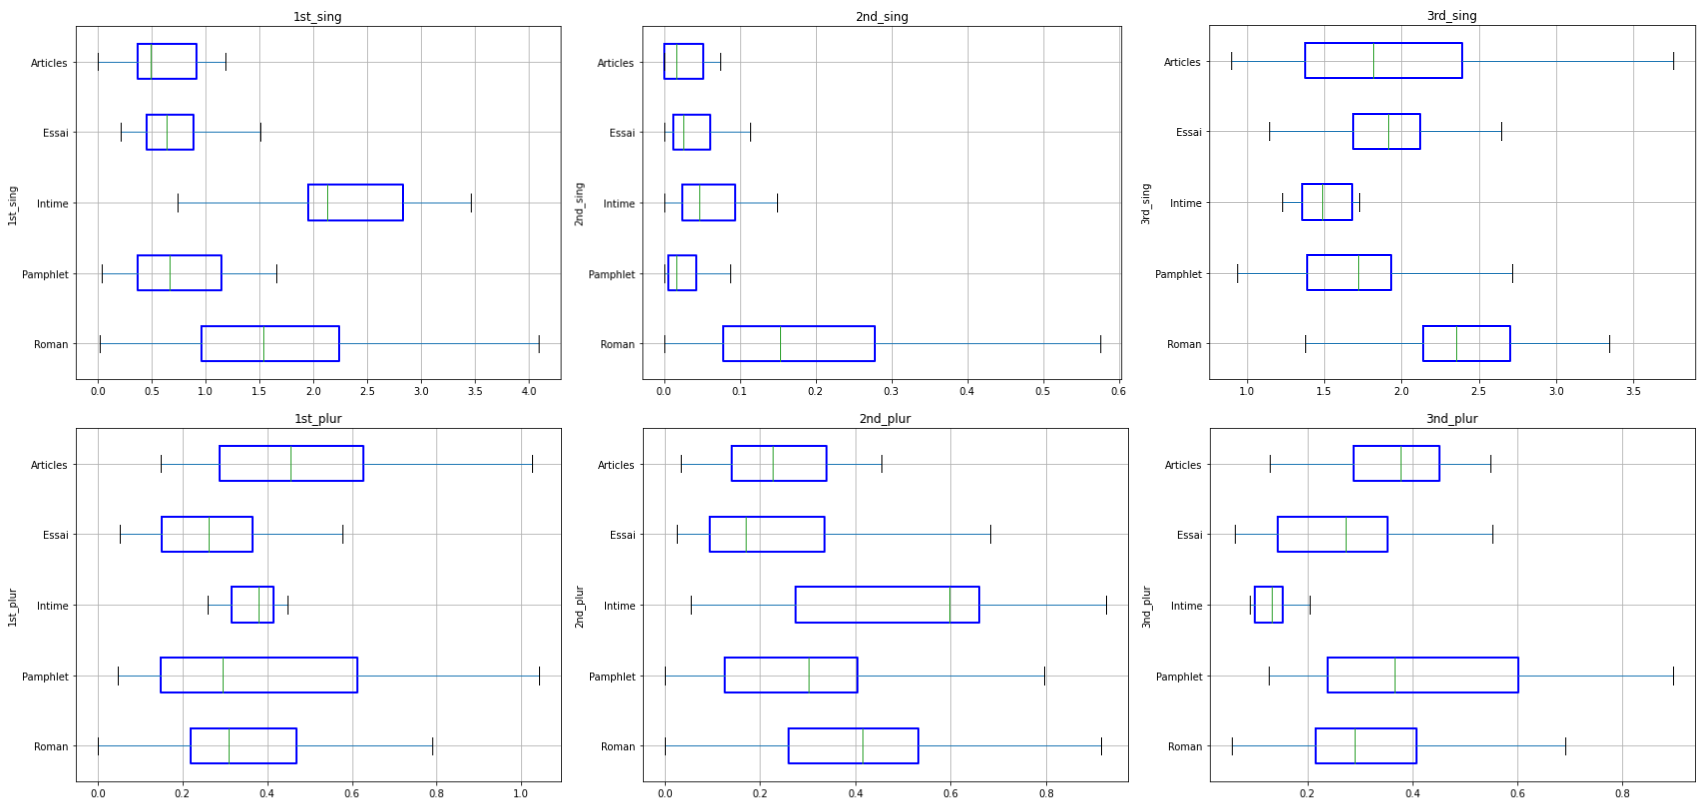
\includegraphics[width=1\textwidth]{img/boxplot_pronoms.png}
\caption{Boite à moustache de la fréquence relative des genres par pronoms}
\label{sortieboitemoustachepronoms}
\end{figure}

\section{Conclusion}

Les résultats ne montrent pas entre le pamphlet et l'essai de différente flagrante sur l'emploi des pronoms. Nous aurions souhaité pouvoir approfondir cette analyse avec la recherche de syntagme plus complexe tel que les suites de \enquote{pronom pronom verbe conjugé} pour avoir un regard plus fin sur la relation des différentes instance de la locution. Avec la librairie Spacy en python, il est possible de rechercher des occurences de \enquote{part-of-speech} ou \enquote{partie de discours} commme avec : \par

    \enquote{[{"TEXT": {"in":["je","tu","il","elle","nous","vous","ils","elles"]}}, {"TEXT": {"in": ["me", "m'","te","t'","le","l'","lui","la","nous","vous","les","s'","leurs"]}}, {"POS":"VERB"}],}

Nous aurions obtenu une matrice combinatoire de tous les emplois des doubles pronoms personnels avant une verbe. Cela aurait pu permettre une analyse factorielle pour discriminer les genres sur l'enjeu de l'énonciation.

\chapter{Recherche de \enquote{motifs} génériques}

\section{Définition des \enquote{motifs}}

Cette seconde partie s'attèle à définir et détecter des motifs distinctifs du genre pamphlétaire. Cela passe par la detection d'occurences lexico-grammaticales caractérisant le style collectif des pamphlétaires. Nous nous appuyons sur le travail de D. Legallois, T. Charnois et T. Poibeau sur l'application de la méthode des motifs du clichés dans les romans sentimentaux\footcites{legallois_reperer_2016}. L'intérêt de cette méthode de detection tient à ce que les formes du cliché sont justement un signe distinctif du roman sentimental\footcites{van_cranenburgh_cliche_nodate}. Pour ce qui est du genre pamphlétaire, nous pensons que le registre polémique et le recours à l'invective puisse être le lieu de formules (motifs) lexicales et grammaticales partagé par une majorité des textes du genre. Nous appliquerons donc une méthode similaire à celle de l'article sur \footcites{legallois_reperer_2016}. Si le cliché est une forme fixe et figée, les auteurs recourt aussi à la detection de forme souple avec des patrons syntaxiques partageant des classes lexicales. \par
Nous appelons \enquote{motifs} des ngrams qui se suivent et se répètent dans un texte ou un corpus de texte. Thierry Poibeau et al.\footcites{legallois_reperer_2016} ont traité cette question des motifs autour du cliché dans les romans sentimentaux. Nous nous inspirons de ce travail pour dans notre cas rechercher des motifs qui soient propres aux textes de pamphlet. Les motifs peuvent être les ngrams de mots mais il est plus intéressant des généraliser l'approche des motifs en modifiant les mots lexicalisés en \textit{part-of-speech}, c'est-à-dire par nature des mots grammaticales. Nous remplaçons dans le corpus de texte les noms, adjectifs, verbes et noms propres en l'indication de leur nature de mots. Cela ajoute une souplesse à la recherche générique de motifs.

\section{Méthode choisie et préparation d'un corpus spécifique}

Pour réaliser cette recherche de motifs nous allons générer nos textes avec la grammaticalisation des noms, adjectifs, verbes et noms propres. Nous effectuons cela avec la librairie Spacy en python. Nous avons tester différents longueur de nombre de mots, les sexto-grammes de mots semblent être le meilleur compromis entre les ressources allouables au calcul et la bonne généralisation de la SVM. Voici un exemple de la sortie des textes avant et après modification : \par

\enquote{Oui, mon Dieu, pour quoi faire, la liberté ? Et pour quoi faire, les pays libres ou réputés tels, la France et ses sœurs d’Europe, pour qui cet idéal de liberté constitue le principal héritage des vieilles chrétientés européennes ?}\textit{La Liberté pour quoi faire ?}, Bernanos\par

\enquote{NOUN , mon PROPN , pour quoi VERB , la NOUN ? Et pour quoi VERB , les NOUN ADJ ou ADJ ADJ , la PROPN et ses NOUN PROPN , pour qui cet ADJ de NOUN VERB le ADJ NOUN des ADJ NOUN ADJ ?}\textit{La Liberté pour quoi faire ?}, Bernanos\par

Nous entraînons avec Superstyl un modèle pour généraliser la classification des textes. Nous extrayons les motifs reconnus comme les plus pertinent pour définir le pamphlet. Nous rechercherons dans les textes la liste des motifs non grammaticalisé en espérant pouvoir analyser une composante stylistique commune.
Pour appliquer cette méthode, nous ne conservons que trois ensemble du corpus 2 défini précédemment, c'est à dire les essais, les romans et les pamphlets de nos auteurs pamphlétaires. Nous délaissons les nouvelles, mémoires et biographies ainsi que les articles car leur distinction avec les pamphlets est plus facilement établi. Nous conservons le roman comme référence très éloignée et le genre de l'essai pour leur grande proximité avec le pamphlet (ce que nous constations précédemment). Pour équilibrer nos classes nous échantillonnons les textes tous les 10000 mots.


\section{Résultats et analyse}

Les résultats de la SVM de la \textit{table \ref{'tab:SVMcorpus2restreint'}} avec les sextogrammes de mots, dont les mots lexicalisés sont grammaticalisés, sont moins bons que ce que nous avons pu obtenir avec les trigrammes de mots simples. Les classes essai et pamphlet sont les moins bien reconnues, néanmoins leurs f1-score restent suffisant pour considérer que le modèle reconnaît les sextogrammes comme cohérent pour généraliser une classification.

\begin{table}[H]
    \centering 
    \begin{tabular}{l c c c c}
        \toprule
             & precision & recall & f1-score & support \\
        \toprule
        \midrule
        roman & 0.87 & 0.92 & 0.90 & 612 \\
        \midrule
        essai & 0.71 & 0.72 & 0.72 & 270\\
        \midrule
        pamphlet & 0.77 & 0.67 & 0.72 & 284\\
        \midrule
        & & & & \\
        \midrule
        accuracy & & & \textbf{0.81} & 1166 \\
        \midrule
        macro-average & 0.79 & 0.77 & 0.78 & 1166\\
        \midrule
        weighted average & 0.81 & 0.81 & 0.81 & 1166\\

        \bottomrule
    \end{tabular}
\caption{Sortie de la SVM sur corpus 2 restreint échantillonné, 6grammes de motifs, LOOCV, class-weight}
\label{'tab:SVMcorpus2restreint'}
\end{table} 
Nous prenons les sextogrammes les plus spécifiques du genre du pamphlet distinct de la classe essai et roman que nous observons sur la figure \ref{'fig:coefs_pamphlet_corpus2restreint'} des coefficients du modèle SVM. 

\begin{figure}[H]
\centering %
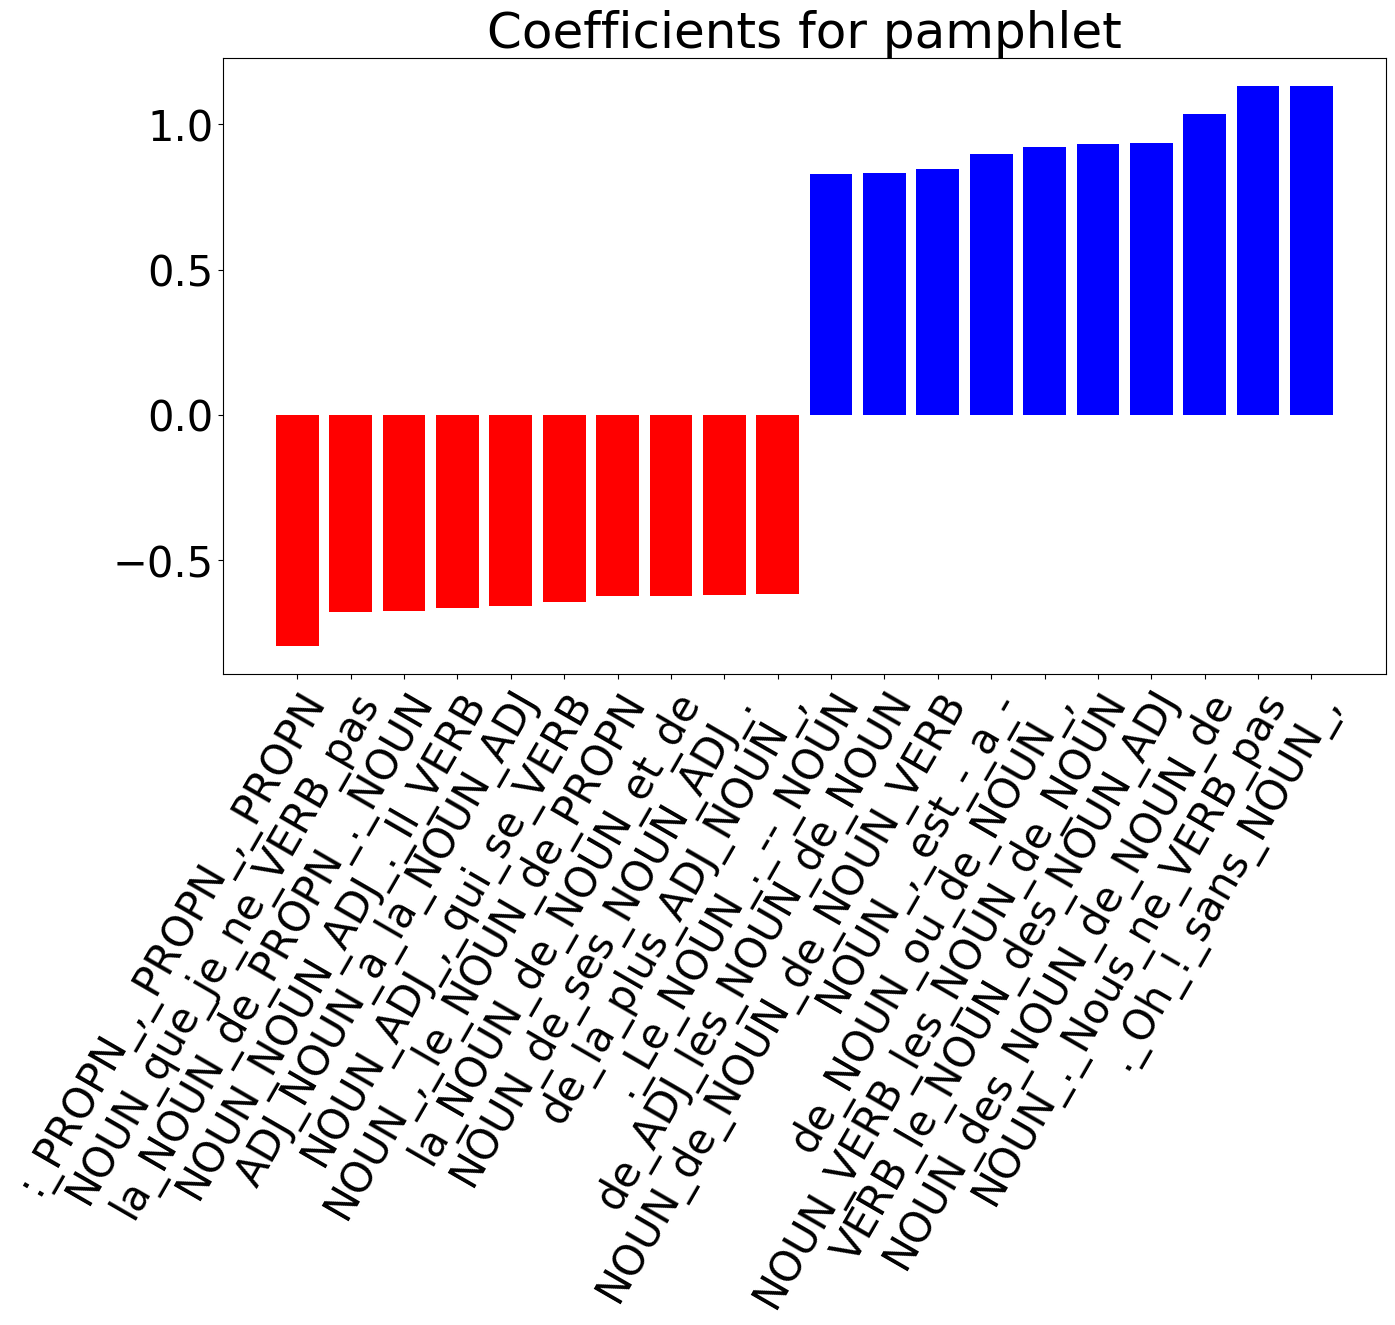
\includegraphics[width=0.70\textwidth]{img/coefs_pamphlet_corpus2restreint.png}
\caption{\textit{Diagramme à barres des coefficients de la classe pamphlet du corpus 2 restreint de motifs}}
\label{'fig:coefs_pamphlet_corpus2restreint'}
\end{figure}

\begin{figure}[H]
\centering %
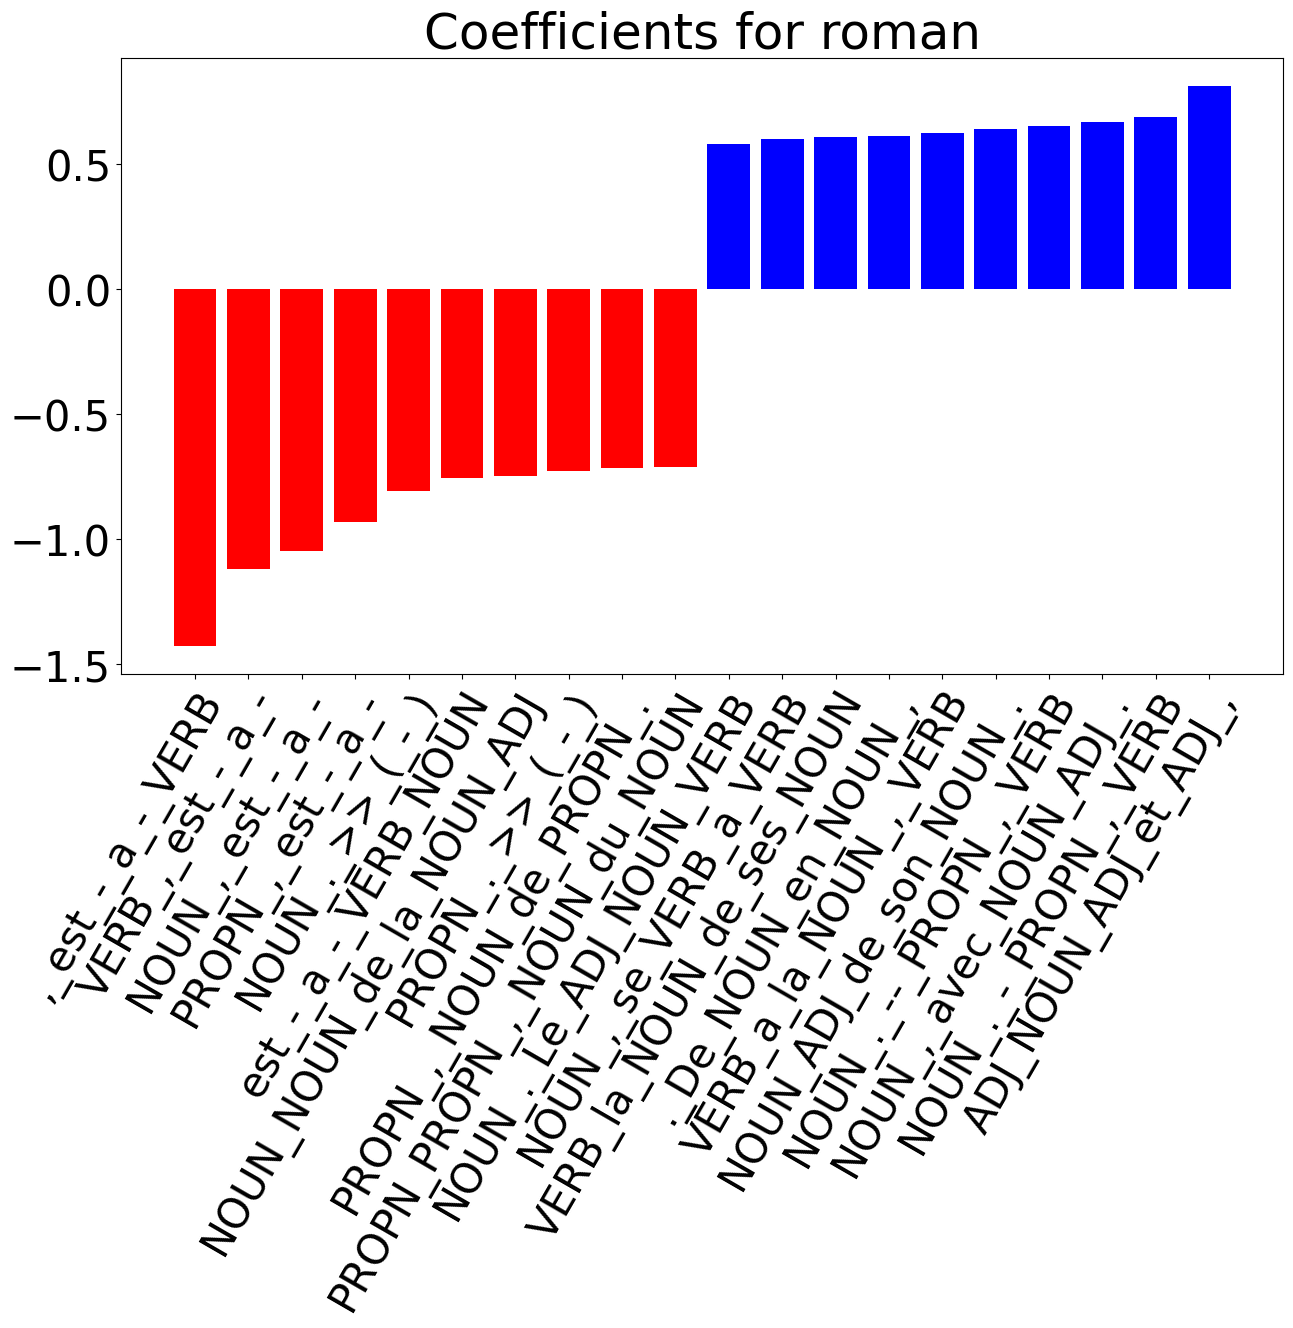
\includegraphics[width=0.70\textwidth]{img/coefs_roman_corpus2restreint.png}
\caption{\textit{Diagramme à barres des coefficients de la classe roman du corpus 2 restreint de motifs}}
\label{'fig:coefs_roman_corpus2restreint'}
\end{figure}

\begin{figure}[H]
\centering %
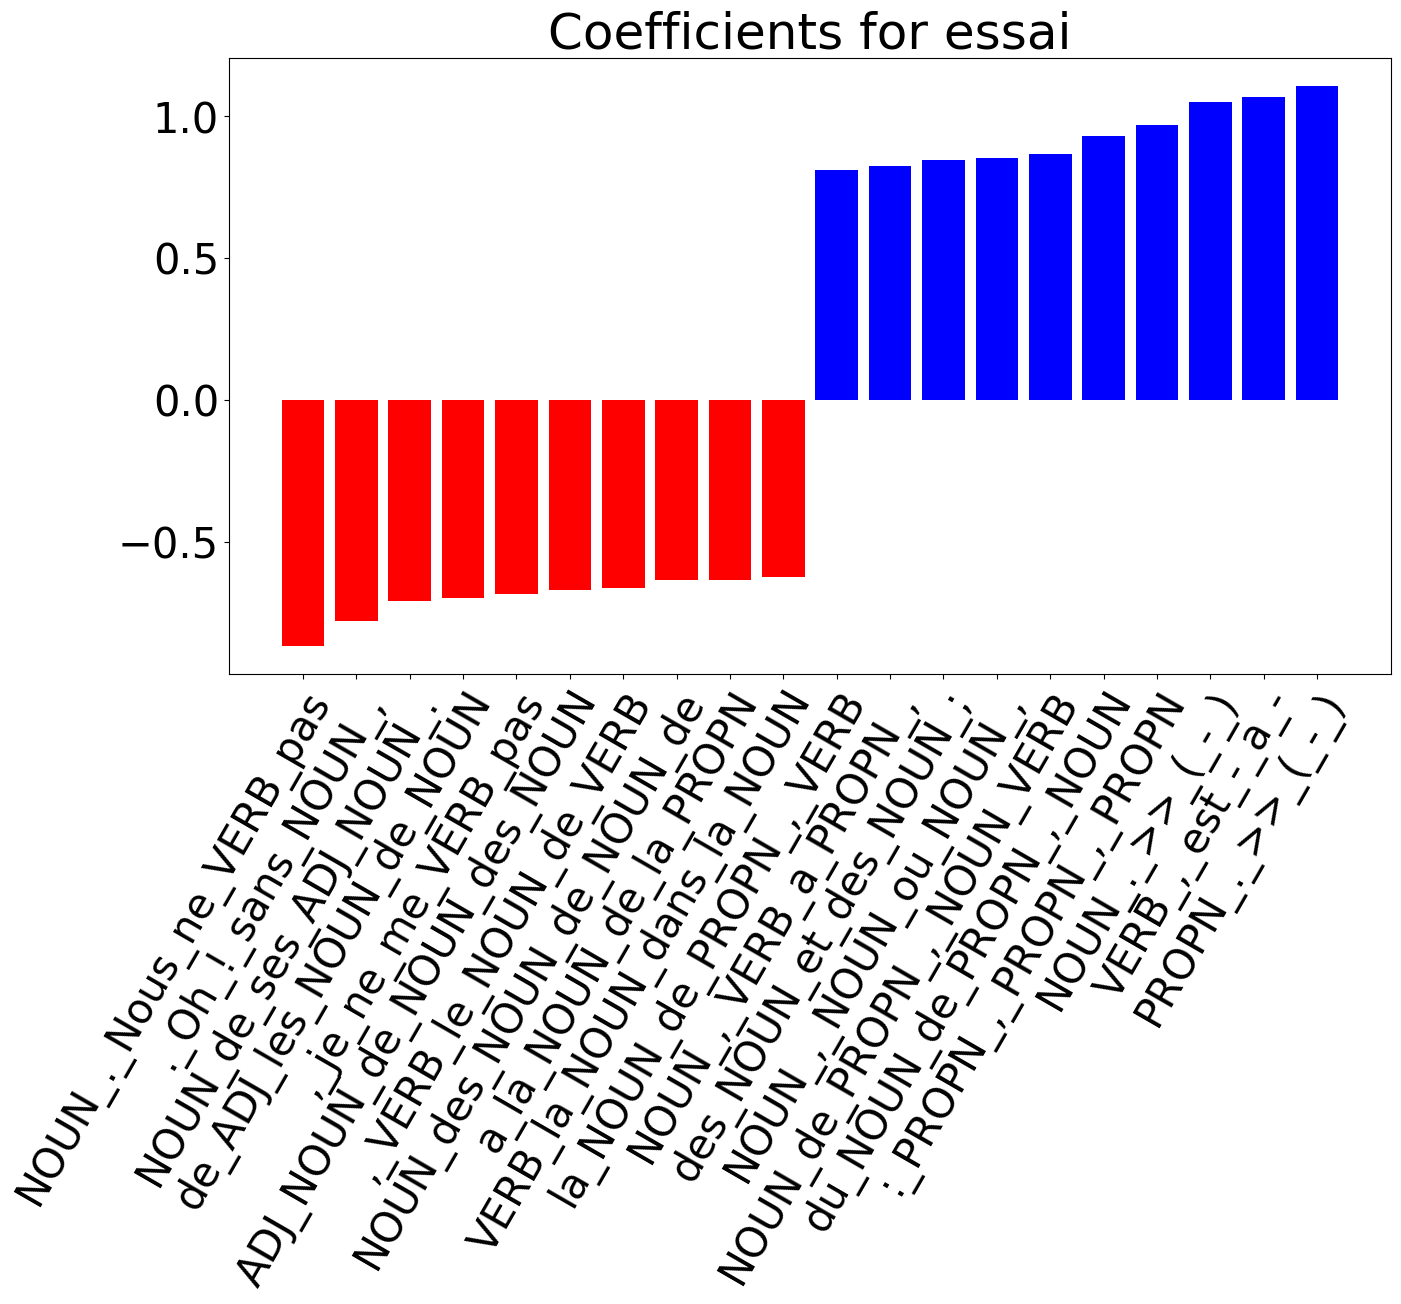
\includegraphics[width=0.70\textwidth]{img/coefs_essai_corpus2restreint.png}
\caption{\textit{Diagramme à barres des coefficients de la classe essai du corpus 2 restreint de motifs}}
\label{'fig:coefs_essai_corpus2restreint'}
\end{figure}

Nous présentons avec la \textit{table \ref{'tab:NOUNoudeNOUN'}} un exemple de ce qu'un des motifs peux dévoiler lorsque l'on recherche les valeurs propres non grammaticalisées dans les textes. La forme déterminant/nom/ou/déterminant/nom dévoile une structure binaire a deux valeur. Soit par opposition comme \enquote{\textit{de vie ou de mort}}, \enquote{\textit{de gré ou de force}} et \enquote{\textit{de paysans ou de bourgeois}}, soit par amplification ou requalification tel \enquote{\textit{de duché ou de comté}}, \enquote{\textit{de médisances ou de calomnies}} et \enquote{\textit{de traîtres ou de lâches}}. Il est intéréssant de voir qu'à travers un même syntagme, différents emplois soit possible.

\newgeometry{left=0.5cm, right=0.5cm}
\begin{longtable}{| p{12.5cm}| c | c| }
    \centering
        \textbf{Match Texte} & \textbf{Nom du Fichier} \\
        \hline
        de système ou de parti & pamphlet\_Bernanos\_La liberté, pour quoi faire \\
        \hline
        de hausse ou de baisse & pamphlet\_Chirac\_Les rois de la République I \\
        \hline
        de tour ou de collection & pamphlet\_Barrès\_Une visite à l’armée anglaise \\
        \hline
        de banditisme ou de forfaiture & pamphlet\_Bloy\_Je m’accuse \\
        \hline
        de vie ou de mort & pamphlet\_Darien\_La Belle France \\
        \hline
        de traîtres ou de lâches & pamphlet\_Bernanos\_Les Grands Cimetières sous la lune \\
        \hline
        de fête ou de dimanche & pamphlet\_Taxil\_Les Pornographes sacrés \\
        \hline
        de régénération ou de destruction & pamphlet\_Taxil\_Les frères Trois-Points \\
        \hline
        de monuments ou de ruines & pamphlet\_Céline\_Mea Culpa \\
        \hline
        de crainte ou de scrupules & pamphlet\_Barrès\_Scènes Et Doctrines Du Nationalisme \\
        \hline
        de variole ou de choléra & pamphlet\_Céline\_Les beaux draps \\
        \hline
        de chefs ou de camarades & pamphlet\_Barrès\_Les Diverses familles spirituelles de la France \\
        \hline
        de croix ou de fleur & pamphlet\_Taxil\_La lanterne d’un suspendu \\
        \hline
        de rouge ou de noir & pamphlet\_Bernanos\_Le crépuscule des vieux \\
        \hline
        de coalitions ou de collusions & pamphlet\_Darien\_Les Vrais Sous-Offs \\
        \hline
        de grains ou de fruits & pamphlet\_Tailhade\_La Noire Idole \\
        \hline
        de perles ou de diamants & pamphlet\_Chirac\_L'agiotage sous la troisième république I \\
        \hline
        de lait ou de pain & pamphlet\_Céline\_Bagatelles pour un massacre \\
        \hline
        de races ou de religions & pamphlet\_Taxil\_À bas la calotte \\
        \hline
        de pions ou de dévotes & pamphlet\_Bernanos\_Où allons-nous \\
        \hline
        de gré ou de force & pamphlet\_Chirac\_L'agiotage sous la troisième république II \\
        \hline
        de chômage ou de bas & pamphlet\_Bernanos\_La France contre les robots \\
        \hline
        de couleur ou de passion & pamphlet\_Tailhade\_À Travers les Grouins \\
        \hline
        de concorde ou de discorde & pamphlet\_Daudet\_La France en alarme \\
        \hline
        de paysans ou de bourgeois & pamphlet\_Vallès\_L'argent \\
        \hline
        de rue ou de café & pamphlet\_Bernanos\_La révolte de l'esprit \\
        \hline
        de comédies ou de drames & pamphlet\_Bloy\_Propos d’un entrepreneur de démolitions \\
        \hline
        de cirage ou de savonnette & pamphlet\_Bernanos\_Le Chemin de la Croix-des-âmes \\
        \hline
        de créancier ou de débiteur & pamphlet\_Chirac\_Les Mystères du crédit \\
        \hline
        de goujatisme ou de piedplatisme & pamphlet\_Bloy\_Devant les cochons \\
        \hline
        de rentes ou de titres & pamphlet\_Tailhade\_Au pays du Mufle \\
        \hline
        de duché ou de comté & pamphlet\_Chirac\_Les rois de la République II \\
        \hline
        de stoïques ou de saints & pamphlet\_Bernanos\_Les enfants humiliés  \\
        \hline
        de chantiers ou de terrains & pamphlet\_Bloy\_Exégèse des lieux communs \\
        \hline
        de guerre ou de salut & pamphlet\_Bernanos\_Francais si vous saviez \\
        \hline
        de droite ou de gauche & pamphlet\_Céline\_L'École des cadavres \\
        \hline
        de cour ou de cuisine & pamphlet\_Chirac\_Erreur commise au préjudice du Trésor français \\
        \hline
        de médisances ou de calomnies & pamphlet\_Taxil\_Mémoires d’une ex-palladiste parfaite, initiée, indépendante \\
        \hline
        de ministre ou de rapporteur & pamphlet\_Chirac\_Les pots de vin parlementaires \\
        \hline
    \caption{Liste de NOUN ou de NOUN pamphlet}
    \label{'tab:NOUNoudeNOUN'}
\end{longtable}


\section{Conclusion}

Nous aurions aimé aller beaucoup plus loin sur cette analyse des motifs, notamment en associant automatiquement les termes lexicalisés à des thèmes en vectorisant les noms, adjectifs et verbes et les plaçant sur des échelles de valeurs comme noble/ignoble, insultant/laudateur et autre. Nous aurions utilisé la librairie Gensim en python pour cela. Cela aurait permis de maximiser la recherche de motifs en associant des valeurs thématiques à des motifs grammaticaux, apportant une dimension de différentes connotations aux motifs.
\chapter{Conclusion générale}

\section{Conclusion}

Pour résumé le propos de cette étude, nous avons déployé différents outils en employant une démarche hypothético-déductive sur l'aspect générique du pamphlet. Notre point de départ fut basé sur le travail de Cédric Passard et de Marc Angenot qui tout deux ont contribués à renouveller les études sur le phénomène du pamphlet. Nos méthodes quantitatives ont nécéssités d'aggréger un grand nombre de texte. Pour cela nous avons constitué différents corpus de texte propre à chacun des choix méthodologiques. 

Nous avons utilisé un classifieur SVM pour détecter les occurrences de classes associables aux genres du roman, de l'essai, de la nouvelle, de l'article, des mémoires et biographies et d'un ensemble de pamphlet. Deux corpus distinct on servi l'un a comparer des textes de pamphlet face à une multitude d'autres genres d'autres auteurs, et l'autre à comparer des genres différents dont le pamphlet sur un même groupe restreint d'auteurs pamphlétaires.
Nous avons pu observer conformément à nos attentes une distinction nette entre ces classes notamment entre les genres narratifs et le pamphlet dans les deux corpus. Une distinction plus fine existe entre le genre de l'essai et le pamphlet pour notre second corpus, le seul à comporter des essais.
À partir de cela nous avons poursuivi notre recherche en nous tournant vers des méthodes non supervisées tel le \textit{clustering ascendant hiérarchique} et l'analyse en composantes principales. Cette seconde salve d'analyse fut propice à mieux cerner la proximité des textes les uns pour les autres et de pouvoir spatialiser la distance qui les séparent ou les rapprochent. La similarité autoriale expliqua beaucoup les rapprochements des oeuvres mais à part pour la comparaison du pamphlet et de l'essai, la majorité des genres se distinguèrent nettement visuellement. Nous avons vu apparaître un groupe de pamphlet se détacher fortement de l'ensemble pamphlétaire, ce qui fait de ces textes un ensemble spécieux de pamphlet qui n'en sont pas entièrement.
Ces deux approches supervisées et non supervisées on montré que si le pamphlet se distingue aisément de différents genre, l'essai sont plus proche parent dans notre corpus est assimilable voir dans le cas des analyses non-supervisées, indiscernable du pamphlet.

Nous avons tenté de développer les spécificités de l'énonciation pamphlétaire pour pouvoir quantitativement constater une distinction du pamphlet et de l'essai. Notre méthode trop rigide n'a pas permis de constater un écart significatif entre ces deux ensembles. 
Une dernière méthode de recherche de syntagme générique ou recherche de motifs à été effectué pour voir poindre des structures proche d'un style collectif des textes pamphlétaire et les premiers résultats encourageant mériteraient d'être approfondis.

En somme, cette étude bien qu'infructueuse a permis de déployer un dialogue entre des méthodes quantitatives très diverse et une réflexion linguistique et stylistique sur les spécificités génériques des textes.

\section{Ouverture}


De nombreuses réflexions laissées à l'état d'ébauche mériteraient une poursuite et un approfondissement. Notamment sur la recherche des aspects spécifiques de l'énonciation par la comparaison de l'usage des pronoms. Nous imaginons très bien une visualisation en réseaux dont les différents noeuds serait les instances locutoires et dont les arrêtes seraient la fréquence des adresses des pronoms personnels sujets vers les pronoms personnels complément d'objet indirect. Nous pourrions y constater des autoréférences comme avec enquote{vous vous trompez} et des réseaux de distribution et de flux distinct en fonction des genres.

Pour l'ébauche d'analyse des motifs, nous aurions souhaité implémenter la méthode suivi par T. Poibeau et al dans l'analyse du cliché, avec la base de l’indice statistique de l’Information Mutuelle pour extraire nos descripteurs. 
Ainsi ce travail n'est pas achevé et appelle une analyse approfondie des structures syntagmatiques pouvant avoir un impact générique plus grand que celui du signal autorial.

% annexes
\chapter{Annexes}

\newgeometry{left=0.5cm, right=0.5cm}
\begin{longtable}{| p{12.5cm}| c | c| }
        \textbf{Nom de l'échantillon} & \textbf{Classe réelle} & \textbf{Classe prédite} \\
        \hline
        mémoire et bio.\char`_Audoux Marguerite\char`_Marie-Claire\char`_sample\char`_1.txt & mémoire et bio. & nouvelle \\
        \hline
        mémoire et bio.\char`_Audoux Marguerite\char`_Marie-Claire\char`_sample\char`_3.txt & mémoire et bio. & nouvelle \\
        \hline
        mémoire et bio.\char`_Barbara Charles\char`_L'assassinat du pont rouge\char`_sample\char`_1.txt & mémoire et bio. & roman \\
        \hline
        mémoire et bio.\char`_Bazin René\char`_La Sarcelle Bleue\char`_sample\char`_1.txt & mémoire et bio. & nouvelle \\
        \hline
        mémoire et bio.\char`_Bazin René\char`_La Sarcelle Bleue\char`_sample\char`_3.txt & mémoire et bio. & nouvelle \\
        \hline
        mémoire et bio.\char`_Belot Adolphe\char`_Alphonsine\char`_sample\char`_2.txt & mémoire et bio. & roman \\
        \hline
        mémoire et bio.\char`_Belot Adolphe\char`_Alphonsine\char`_sample\char`_3.txt & mémoire et bio. & roman \\
        \hline
        mémoire et bio.\char`_Boylesve René\char`_Le carrosse aux deux lézards verts\char`_sample\char`_1.txt & mémoire et bio. & nouvelle \\
        \hline
        mémoire et bio.\char`_Boylesve René\char`_Le carrosse aux deux lézards verts\char`_sample\char`_2.txt & mémoire et bio. & roman \\
        \hline
        mémoire et bio.\char`_Daudet Alphonse\char`_Souvenirs d'un homme de lettres\char`_sample\char`_1.txt & mémoire et bio. & nouvelle \\
        \hline
        mémoire et bio.\char`_Daudet Alphonse\char`_Wood'stown\char`_sample\char`_1.txt & mémoire et bio. & nouvelle \\
        \hline
        mémoire et bio.\char`_Dubut de Laforest Jean-Louis\char`_Morphine\char`_sample\char`_2.txt & mémoire et bio. & nouvelle \\
        \hline
        mémoire et bio.\char`_Dubut de Laforest Jean-Louis\char`_Morphine\char`_sample\char`_3.txt & mémoire et bio. & nouvelle \\
        \hline
        mémoire et bio.\char`_Dumas (père) Alexandre\char`_La boule de neige\char`_sample\char`_3.txt & mémoire et bio. & nouvelle \\
        \hline
        mémoire et bio.\char`_Dumas (père) Alexandre\char`_La boule de neige\char`_sample\char`_4.txt & mémoire et bio. & roman \\
        \hline
        mémoire et bio.\char`_Dumas (père) Alexandre\char`_Une aventure d'amour\char`_sample\char`_2.txt & mémoire et bio. & roman \\
        \hline
        mémoire et bio.\char`_Durand Alice dite Gréville Henry\char`_Croquis\char`_sample\char`_3.txt & mémoire et bio. & nouvelle \\
        \hline
        mémoire et bio.\char`_Durand Alice dite Gréville Henry\char`_Croquis\char`_sample\char`_4.txt & mémoire et bio. & nouvelle \\
        \hline
        mémoire et bio.\char`_Eekhoud Georges\char`_La faneuse d'amour\char`_sample\char`_1.txt & mémoire et bio. & nouvelle \\
        \hline
        mémoire et bio.\char`_Eekhoud Georges\char`_La faneuse d'amour\char`_sample\char`_3.txt & mémoire et bio. & nouvelle \\
        \hline
        mémoire et bio.\char`_Eekhoud Georges\char`_La faneuse d'amour\char`_sample\char`_4.txt & mémoire et bio. & nouvelle \\
        \hline
        mémoire et bio.\char`_Feuillet Octave\char`_La petite comtesse\char`_sample\char`_1.txt & mémoire et bio. & roman \\
        \hline
        mémoire et bio.\char`_Féval Paul (père)\char`_La Ville-Vampire (ou bien le malheur d’écrire des romans noirs)\char`_sample\char`_2.txt & mémoire et bio. & nouvelle \\
        \hline
        mémoire et bio.\char`_Féval Paul (père)\char`_La Ville-Vampire (ou bien le malheur d’écrire des romans noirs)\char`_sample\char`_4.txt & mémoire et bio. & roman \\
        \hline
        mémoire et bio.\char`_Féval (père) Paul\char`_La fabrique de crimes\char`_sample\char`_1.txt & mémoire et bio. & roman \\
        \hline
        mémoire et bio.\char`_Galopin Arnould\char`_La ténébreuse affaire de Green-Park\char`_sample\char`_2.txt & mémoire et bio. & nouvelle \\
        \hline
        mémoire et bio.\char`_Galopin Arnould\char`_La ténébreuse affaire de Green-Park\char`_sample\char`_3.txt & mémoire et bio. & nouvelle \\
        \hline
        mémoire et bio.\char`_Gay Sophie\char`_Anatole, Vol. 2\char`_sample\char`_2.txt & mémoire et bio. & roman \\
        \hline
        mémoire et bio.\char`_Gérald-Montméril (pseud. Gérald Mabel et Mme Mairel d'Eslon)\char`_Chryséis au désert\char`_sample\char`_1.txt & mémoire et bio. & nouvelle \\
        \hline
        mémoire et bio.\char`_Gérald-Montméril (pseud. Gérald Mabel et Mme Mairel d'Eslon)\char`_Chryséis au désert\char`_sample\char`_3.txt & mémoire et bio. & nouvelle \\
        \hline
        mémoire et bio.\char`_Gérald-Montméril (pseud. Gérald Mabel et Mme Mairel d'Eslon)\char`_Chryséis au désert\char`_sample\char`_4.txt & mémoire et bio. & roman \\
        \hline
        mémoire et bio.\char`_Ginouvier J.-F.-T.\char`_Gustave et Aspaïs, ou Les victimes des préjugés de l'époque . Par T. Ginouvier - Tome 2 (1826)\char`_sample\char`_3.txt & mémoire et bio. & pamphlet \\
        \hline
        mémoire et bio.\char`_Hémon Louis\char`_Écrits sur le Québec\char`_sample\char`_2.txt & mémoire et bio. & pamphlet \\
        \hline
        mémoire et bio.\char`_Inconnu\char`_Indiscrétions d'une Parisienne. Mademoiselle Figaro (1880)\char`_sample\char`_1.txt & mémoire et bio. & nouvelle \\
        \hline
        mémoire et bio.\char`_Inconnu\char`_Indiscrétions d'une Parisienne. Mademoiselle Figaro (1880)\char`_sample\char`_2.txt & mémoire et bio. & roman \\
        \hline
        mémoire et bio.\char`_Inconnu\char`_Indiscrétions d'une Parisienne. Mademoiselle Figaro (1880)\char`_sample\char`_3.txt & mémoire et bio. & roman \\
        \hline
        mémoire et bio.\char`_Lermina Jules\char`_La deux fois morte\char`_sample\char`_1.txt & mémoire et bio. & nouvelle \\
        \hline
        mémoire et bio.\char`_Lermina Jules\char`_L'énigme\char`_sample\char`_1.txt & mémoire et bio. & nouvelle \\
        \hline
        mémoire et bio.\char`_Loti Pierre\char`_Figures et choses qui passaient\char`_sample\char`_3.txt & mémoire et bio. & nouvelle \\
        \hline
        mémoire et bio.\char`_Loti Pierre\char`_Matelot\char`_sample\char`_1.txt & mémoire et bio. & nouvelle \\
        \hline
        mémoire et bio.\char`_Loti Pierre\char`_Matelot\char`_sample\char`_3.txt & mémoire et bio. & nouvelle \\
        \hline
        mémoire et bio.\char`_Maupassant Guy de\char`_Au soleil\char`_sample\char`_2.txt & mémoire et bio. & nouvelle \\
        \hline
        mémoire et bio.\char`_Maupassant Guy de\char`_Au soleil\char`_sample\char`_3.txt & mémoire et bio. & nouvelle \\
        \hline
        mémoire et bio.\char`_Mazier du Heaume Hippolyte\char`_Voyage d'un jeune grec à Paris. Volume 2\char`_sample\char`_1.txt & mémoire et bio. & pamphlet \\
        \hline
        mémoire et bio.\char`_Méténier Oscar\char`_Le gorille. Roman parisien\char`_sample\char`_1.txt & mémoire et bio. & roman \\
        \hline
        mémoire et bio.\char`_Méténier Oscar\char`_Le gorille. Roman parisien\char`_sample\char`_2.txt & mémoire et bio. & nouvelle \\
        \hline
        mémoire et bio.\char`_Méténier Oscar\char`_Le gorille. Roman parisien\char`_sample\char`_3.txt & mémoire et bio. & roman \\
        \hline
        mémoire et bio.\char`_Musset Paul de\char`_La Chèvre Jaune\char`_sample\char`_1.txt & mémoire et bio. & nouvelle \\
        \hline
        mémoire et bio.\char`_Musset Paul de\char`_La Chèvre Jaune\char`_sample\char`_2.txt & mémoire et bio. & nouvelle \\
        \hline
        mémoire et bio.\char`_Nadaud Marcel\char`_Chignole (la guerre aérienne)\char`_sample\char`_1.txt & mémoire et bio. & nouvelle \\
        \hline
        mémoire et bio.\char`_Nervo Robert de (Baron)\char`_Les Mémoires de mon coupé (1881)\char`_sample\char`_2.txt & mémoire et bio. & nouvelle \\
        \hline
        mémoire et bio.\char`_Nizan Paul\char`_Aden Arabie\char`_sample\char`_1.txt & mémoire et bio. & pamphlet \\
        \hline
        mémoire et bio.\char`_Nizan Paul\char`_Aden Arabie\char`_sample\char`_2.txt & mémoire et bio. & pamphlet \\
        \hline
        mémoire et bio.\char`_Nizan Paul\char`_Aden Arabie\char`_sample\char`_3.txt & mémoire et bio. & pamphlet \\
        \hline
        mémoire et bio.\char`_Ohnet Georges\char`_L'Ame de Pierre\char`_sample\char`_1.txt & mémoire et bio. & nouvelle \\
        \hline
        mémoire et bio.\char`_Ohnet Georges\char`_L'Ame de Pierre\char`_sample\char`_2.txt & mémoire et bio. & nouvelle \\
        \hline
        mémoire et bio.\char`_Ohnet Georges\char`_L'Ame de Pierre\char`_sample\char`_3.txt & mémoire et bio. & roman \\
        \hline
        mémoire et bio.\char`_Pollet Louis Léonard dit Corday Michel\char`_Les révélées\char`_sample\char`_1.txt & mémoire et bio. & nouvelle \\
        \hline
        mémoire et bio.\char`_Pollet Louis Léonard dit Corday Michel\char`_Les révélées\char`_sample\char`_2.txt & mémoire et bio. & nouvelle \\
        \hline
        mémoire et bio.\char`_Ponson du Terrail Pierre\char`_Le Chambrion\char`_sample\char`_1.txt & mémoire et bio. & roman \\
        \hline
        mémoire et bio.\char`_Renard Jules\char`_Poil de carotte\char`_sample\char`_2.txt & mémoire et bio. & nouvelle \\
        \hline
        mémoire et bio.\char`_Rodenbach Georges\char`_Bruges-la-Morte\char`_sample\char`_1.txt & mémoire et bio. & nouvelle \\
        \hline
        mémoire et bio.\char`_Rosny aîné J-H\char`_La Femme disparue\char`_sample\char`_2.txt & mémoire et bio. & roman \\
        \hline
        mémoire et bio.\char`_Sales Pierre\char`_Le sergent Renaud. Aventures parisiennes\char`_sample\char`_1.txt & mémoire et bio. & roman \\
        \hline
        mémoire et bio.\char`_Sand George\char`_Promenades autour d’un village\char`_sample\char`_2.txt & mémoire et bio. & pamphlet \\
        \hline
        mémoire et bio.\char`_Sand George\char`_Promenades autour d’un village\char`_sample\char`_3.txt & mémoire et bio. & pamphlet \\
        \hline
        mémoire et bio.\char`_Sand George\char`_Promenades autour d’un village\char`_sample\char`_4.txt & mémoire et bio. & pamphlet \\
        \hline
        mémoire et bio.\char`_Signol Alphonse\char`_Le Chiffonnier, par Alphonse Signol et Stanislas Macaire - Tome 3 (1831)\char`_sample\char`_2.txt & mémoire et bio. & roman \\
        \hline
        mémoire et bio.\char`_Signol Alphonse\char`_Le Chiffonnier, par Alphonse Signol et Stanislas Macaire - Tome 4 (1831)\char`_sample\char`_1.txt & mémoire et bio. & roman \\
        \hline
        mémoire et bio.\char`_Tardieu Charles Henri\char`_Lettres de Bayreuth\char`_sample\char`_2.txt & mémoire et bio. & pamphlet \\
        \hline
        mémoire et bio.\char`_Toudouze Gustave\char`_La sirène: souvenir de Capri\char`_sample\char`_1.txt & mémoire et bio. & nouvelle \\
        \hline
        mémoire et bio.\char`_Toulet Paul Jean\char`_La jeune fille verte, roman\char`_sample\char`_3.txt & mémoire et bio. & nouvelle \\
        \hline
        mémoire et bio.\char`_Verlaine Paul\char`_Les mémoires d’un veuf\char`_sample\char`_2.txt & mémoire et bio. & pamphlet \\
        \hline
        mémoire et bio.\char`_Verlaine Paul\char`_Mes hôpitaux\char`_sample\char`_1.txt & mémoire et bio. & pamphlet \\
        \hline
        mémoire et bio.\char`_Verlaine Paul\char`_Mes prisons\char`_sample\char`_1.txt & mémoire et bio. & pamphlet \\
        \hline
        mémoire et bio.\char`_Zaccone Pierre\char`_Éric le mendiant\char`_sample\char`_2.txt & mémoire et bio. & nouvelle \\
        \hline
        mémoire et bio.\char`_Zaccone Pierre\char`_La Dame d'Auteuil\char`_sample\char`_3.txt & mémoire et bio. & roman \\
        \hline
        nouvelle\char`_Allary Camille\char`_Au pays des cigales\char`_sample\char`_2.txt & nouvelle & mémoire et bio. \\
        \hline
        nouvelle\char`_Arène Paul\char`_Contes de Provence\char`_sample\char`_2.txt & nouvelle & mémoire et bio. \\
        \hline
        nouvelle\char`_Balzac Honoré de\char`_El Verdugo\char`_sample\char`_1.txt & nouvelle & roman \\
        \hline
        nouvelle\char`_Balzac Honoré de\char`_Esquisse d’un homme d’affaires d’après nature\char`_sample\char`_1.txt & nouvelle & roman \\
        \hline
        nouvelle\char`_Balzac Honoré de\char`_Gambara\char`_sample\char`_2.txt & nouvelle & roman \\
        \hline
        nouvelle\char`_Balzac Honoré de\char`_Le Bal de Sceaux\char`_sample\char`_1.txt & nouvelle & roman \\
        \hline
        nouvelle\char`_Balzac Honoré de\char`_Le Bal de Sceaux\char`_sample\char`_2.txt & nouvelle & roman \\
        \hline
        nouvelle\char`_Balzac Honoré de\char`_Les Secrets de la princesse de Cadignan\char`_sample\char`_1.txt & nouvelle & roman \\
        \hline
        nouvelle\char`_Balzac Honoré de\char`_Maître Cornélius\char`_sample\char`_1.txt & nouvelle & roman \\
        \hline
        nouvelle\char`_Balzac Honoré de\char`_Une passion dans le désert\char`_sample\char`_1.txt & nouvelle & roman \\
        \hline
        nouvelle\char`_Balzac Honoré de\char`_Z. Marcas\char`_sample\char`_1.txt & nouvelle & roman \\
        \hline
        nouvelle\char`_Bellaud E. de\char`_Ces pauvres filles !\char`_sample\char`_1.txt & nouvelle & roman \\
        \hline
        nouvelle\char`_Bellaud E. de\char`_Ces pauvres filles !\char`_sample\char`_3.txt & nouvelle & roman \\
        \hline
        nouvelle\char`_Boissières Ernest\char`_Un crime inconnu\char`_sample\char`_3.txt & nouvelle & mémoire et bio. \\
        \hline
        nouvelle\char`_Bréhat Alfred de\char`_Le bal de l'Opéra\char`_sample\char`_4.txt & nouvelle & mémoire et bio. \\
        \hline
        nouvelle\char`_Bréhat Alfred de\char`_L'hôtel du dragon ; Souvenirs de voyages\char`_sample\char`_1.txt & nouvelle & mémoire et bio. \\
        \hline
        nouvelle\char`_Bréhat Alfred de\char`_L'hôtel du dragon ; Souvenirs de voyages\char`_sample\char`_3.txt & nouvelle & mémoire et bio. \\
        \hline
        nouvelle\char`_Cim Albert\char`_Contes et souvenirs de mon pays\char`_sample\char`_2.txt & nouvelle & mémoire et bio. \\
        \hline
        nouvelle\char`_Claretie Jules\char`_Bouddha\char`_sample\char`_1.txt & nouvelle & mémoire et bio. \\
        \hline
        nouvelle\char`_Colette\char`_Les Vrilles de la vigne\char`_sample\char`_2.txt & nouvelle & mémoire et bio. \\
        \hline
        nouvelle\char`_Crevel René\char`_Le roman cassé\char`_sample\char`_1.txt & nouvelle & pamphlet \\
        \hline
        nouvelle\char`_Daudet Alphonse\char`_Le Cabecilla\char`_sample\char`_1.txt & nouvelle & mémoire et bio. \\
        \hline
        nouvelle\char`_Daudet Alphonse\char`_Le Père Achille\char`_sample\char`_1.txt & nouvelle & mémoire et bio. \\
        \hline
        nouvelle\char`_Dumas Alexandre (père)\char`_Un coup de feu et autres nouvelles\char`_sample\char`_2.txt & nouvelle & mémoire et bio. \\
        \hline
        nouvelle\char`_Dupin Antoinette\char`_Comment tout finit (tome 1)\char`_sample\char`_3.txt & nouvelle & mémoire et bio. \\
        \hline
        nouvelle\char`_Durand Alice dite Gréville Henry\char`_À travers champs\char`_sample\char`_2.txt & nouvelle & mémoire et bio. \\
        \hline
        nouvelle\char`_Eyma Xavier\char`_Le Médaillon\char`_sample\char`_1.txt & nouvelle & roman \\
        \hline
        nouvelle\char`_Eyma Xavier\char`_Le Médaillon\char`_sample\char`_2.txt & nouvelle & roman \\
        \hline
        nouvelle\char`_France Anatole\char`_Les contes de Jacques Tournebroche\char`_sample\char`_2.txt & nouvelle & mémoire et bio. \\
        \hline
        nouvelle\char`_France Anatole\char`_Nos enfants : scènes de la ville et des champs\char`_sample\char`_1.txt & nouvelle & mémoire et bio. \\
        \hline
        nouvelle\char`_Gautier Judith\char`_Le paravent de soie et d'or\char`_sample\char`_1.txt & nouvelle & mémoire et bio. \\
        \hline
        nouvelle\char`_Giraudoux Jean\char`_L’école des indifférents\char`_sample\char`_1.txt & nouvelle & mémoire et bio. \\
        \hline
        nouvelle\char`_Gourmont Remy de\char`_La petite ville\char`_sample\char`_1.txt & nouvelle & mémoire et bio. \\
        \hline
        nouvelle\char`_Gozlan Léon\char`_Le Capitaine Maubert\char`_sample\char`_2.txt & nouvelle & mémoire et bio. \\
        \hline
        nouvelle\char`_Houssaye Arsène\char`_Les douze nouvelles nouvelles\char`_sample\char`_3.txt & nouvelle & mémoire et bio. \\
        \hline
        nouvelle\char`_Hugo Victor\char`_Claude Gueux\char`_sample\char`_1.txt & nouvelle & roman \\
        \hline
        nouvelle\char`_Jarry Alfred\char`_L'Autre Alceste\char`_sample\char`_1.txt & nouvelle & mémoire et bio. \\
        \hline
        nouvelle\char`_Karr Alphonse\char`_Histoire d'un pion\char`_sample\char`_1.txt & nouvelle & mémoire et bio. \\
        \hline
        nouvelle\char`_Leblanc Maurice\char`_La dent d’Hercule Petitgris\char`_sample\char`_1.txt & nouvelle & roman \\
        \hline
        nouvelle\char`_Leblanc Maurice\char`_Le Cabochon d'émeraude\char`_sample\char`_1.txt & nouvelle & mémoire et bio. \\
        \hline
        nouvelle\char`_Leblanc Maurice\char`_Un gentleman\char`_sample\char`_1.txt & nouvelle & mémoire et bio. \\
        \hline
        nouvelle\char`_Lermina Jules\char`_L'élixir de vie\char`_sample\char`_1.txt & nouvelle & mémoire et bio. \\
        \hline
        nouvelle\char`_Leroux Gaston\char`_L’homme qui a vu le diable\char`_sample\char`_1.txt & nouvelle & mémoire et bio. \\
        \hline
        nouvelle\char`_Le Roux Hugues\char`_Les Gens d'aujourd'hui. Marins et soldats\char`_sample\char`_2.txt & nouvelle & mémoire et bio. \\
        \hline
        nouvelle\char`_Loti Pierre\char`_Fantôme d'Orient\char`_sample\char`_1.txt & nouvelle & mémoire et bio. \\
        \hline
        nouvelle\char`_Loti Pierre\char`_Le livre de la pitié et de la mort\char`_sample\char`_1.txt & nouvelle & mémoire et bio. \\
        \hline
        nouvelle\char`_Loti Pierre\char`_Le livre de la pitié et de la mort\char`_sample\char`_2.txt & nouvelle & mémoire et bio. \\
        \hline
        nouvelle\char`_Loti Pierre\char`_Le livre de la pitié et de la mort\char`_sample\char`_3.txt & nouvelle & mémoire et bio. \\
        \hline
        nouvelle\char`_Mérimée Prosper\char`_Colomba\char`_sample\char`_2.txt & nouvelle & roman \\
        \hline
        nouvelle\char`_Mérimée Prosper\char`_Colomba\char`_sample\char`_3.txt & nouvelle & roman \\
        \hline
        nouvelle\char`_Mérimée Prosper\char`_La Venus d'Ille\char`_sample\char`_1.txt & nouvelle & mémoire et bio. \\
        \hline
        nouvelle\char`_Mérimée Prosper\char`_Mateo Falcone\char`_sample\char`_1.txt & nouvelle & mémoire et bio. \\
        \hline
        nouvelle\char`_Petitjean de la Rosière Jeanne-Marie\char`_Contes\char`_sample\char`_1.txt & nouvelle & roman \\
        \hline
        nouvelle\char`_Pollet Louis Léonard dit Corday Michel\char`_Plaisirs d'auto\char`_sample\char`_1.txt & nouvelle & mémoire et bio. \\
        \hline
        nouvelle\char`_Renard Jules\char`_Bucoliques\char`_sample\char`_3.txt & nouvelle & mémoire et bio. \\
        \hline
        nouvelle\char`_Renard Maurice\char`_Fantômes et Fantoches\char`_sample\char`_1.txt & nouvelle & mémoire et bio. \\
        \hline
        nouvelle\char`_Renard Maurice\char`_L'Homme Truqué\char`_sample\char`_1.txt & nouvelle & mémoire et bio. \\
        \hline
        nouvelle\char`_Renard Maurice\char`_L'Homme Truqué\char`_sample\char`_2.txt & nouvelle & mémoire et bio. \\
        \hline
        nouvelle\char`_Renard Maurice\char`_L'Homme Truqué\char`_sample\char`_3.txt & nouvelle & mémoire et bio. \\
        \hline
        nouvelle\char`_Richardet Gustave\char`_Le Mariage de Bouillardin, suivi de Quatre jours de prison sous la Commune\char`_sample\char`_1.txt & nouvelle & mémoire et bio. \\
        \hline
        nouvelle\char`_Richardet Gustave\char`_Le Mariage de Bouillardin, suivi de Quatre jours de prison sous la Commune\char`_sample\char`_2.txt & nouvelle & mémoire et bio. \\
        \hline
        nouvelle\char`_Rosny Aîné J-H\char`_La tentatrice\char`_sample\char`_1.txt & nouvelle & mémoire et bio. \\
        \hline
        nouvelle\char`_Sand George\char`_Kourroglou\char`_sample\char`_1.txt & nouvelle & roman \\
        \hline
        nouvelle\char`_Sand George\char`_La fauvette du docteur\char`_sample\char`_1.txt & nouvelle & mémoire et bio. \\
        \hline
        nouvelle\char`_Sand George\char`_Melchior\char`_sample\char`_1.txt & nouvelle & roman \\
        \hline
        nouvelle\char`_Schwob Marcel\char`_Le roi au masque d’or\char`_sample\char`_3.txt & nouvelle & mémoire et bio. \\
        \hline
        nouvelle\char`_Souvestre Émile\char`_Dans la prairie\char`_sample\char`_2.txt & nouvelle & roman \\
        \hline
        nouvelle\char`_Souvestre Émile\char`_Dans la prairie\char`_sample\char`_3.txt & nouvelle & roman \\
        \hline
        nouvelle\char`_Tonelli Philippe\char`_Scènes de la vie corse : Seppa\char`_sample\char`_3.txt & nouvelle & mémoire et bio. \\
        \hline
        nouvelle\char`_Verne Jules\char`_Au XXIXe siècle ou la journée d’un journaliste américain\char`_sample\char`_1.txt & nouvelle & mémoire et bio. \\
        \hline
        nouvelle\char`_Villiers de l'Isle-Adam Auguste\char`_Tribulat Bonhomet\char`_sample\char`_1.txt & nouvelle & mémoire et bio. \\
        \hline
        nouvelle\char`_Villiers de l'Isle-Adam Auguste\char`_Tribulat Bonhomet\char`_sample\char`_2.txt & nouvelle & pamphlet \\
        \hline
        pamphlet\char`_Céline\char`_Bagatelles pour un massacre\char`_sample\char`_1.txt & pamphlet & mémoire et bio. \\
        \hline
        pamphlet\char`_Tailhade\char`_La Noire Idole\char`_sample\char`_1.txt & pamphlet & mémoire et bio. \\
        \hline
        roman\char`_Allais Alphonse\char`_L’affaire Blaireau\char`_sample\char`_1.txt & roman & nouvelle \\
        \hline
        roman\char`_Allais Alphonse\char`_L’affaire Blaireau\char`_sample\char`_2.txt & roman & mémoire et bio. \\
        \hline
        roman\char`_Balzac Honoré de\char`_Gaudissart II\char`_sample\char`_1.txt & roman & nouvelle \\
        \hline
        roman\char`_Balzac Honoré de\char`_Gobseck\char`_sample\char`_1.txt & roman & nouvelle \\
        \hline
        roman\char`_Balzac Honoré de\char`_Histoire des Treize : La Fille aux yeux d’or\char`_sample\char`_1.txt & roman & nouvelle \\
        \hline
        roman\char`_Balzac Honoré de\char`_Histoire des Treize : La Fille aux yeux d’or\char`_sample\char`_2.txt & roman & nouvelle \\
        \hline
        roman\char`_Balzac Honoré de\char`_La Fausse Maîtresse\char`_sample\char`_1.txt & roman & nouvelle \\
        \hline
        roman\char`_Balzac Honoré de\char`_La Maison du chat-qui-pelote\char`_sample\char`_1.txt & roman & nouvelle \\
        \hline
        roman\char`_Balzac Honoré de\char`_La Maison Nucingen\char`_sample\char`_1.txt & roman & nouvelle \\
        \hline
        roman\char`_Balzac Honoré de\char`_La Maison Nucingen\char`_sample\char`_2.txt & roman & nouvelle \\
        \hline
        roman\char`_Balzac Honoré de\char`_Le Colonel Chabert\char`_sample\char`_1.txt & roman & nouvelle \\
        \hline
        roman\char`_Balzac Honoré de\char`_Le Colonel Chabert\char`_sample\char`_2.txt & roman & nouvelle \\
        \hline
        roman\char`_Balzac Honoré de\char`_L’Enfant maudit\char`_sample\char`_1.txt & roman & nouvelle \\
        \hline
        roman\char`_Balzac Honoré de\char`_L’Enfant maudit\char`_sample\char`_3.txt & roman & nouvelle \\
        \hline
        roman\char`_Balzac Honoré de\char`_Les Proscrits\char`_sample\char`_1.txt & roman & nouvelle \\
        \hline
        roman\char`_Balzac Honoré de\char`_L’Illustre Gaudissart\char`_sample\char`_1.txt & roman & nouvelle \\
        \hline
        roman\char`_Barbey d'Aurevilly Jules\char`_Le Chevalier des Touches\char`_sample\char`_2.txt & roman & nouvelle \\
        \hline
        roman\char`_Barrès Maurice\char`_Sous l'oeil des barbares. Le culte du moi 1\char`_sample\char`_1.txt & roman & nouvelle \\
        \hline
        roman\char`_Barrès Maurice\char`_Sous l'oeil des barbares. Le culte du moi 1\char`_sample\char`_2.txt & roman & nouvelle \\
        \hline
        roman\char`_Barrès Maurice\char`_Un jardin sur l'Oronte\char`_sample\char`_2.txt & roman & nouvelle \\
        \hline
        roman\char`_David Laurent-Olivier\char`_Le Héros de Châteauguay\char`_sample\char`_1.txt & roman & pamphlet \\
        \hline
        roman\char`_Dumas (père) Alexandre\char`_Jane\char`_sample\char`_2.txt & roman & mémoire et bio. \\
        \hline
        roman\char`_Dumas (père) Alexandre\char`_La colombe\char`_sample\char`_1.txt & roman & mémoire et bio. \\
        \hline
        roman\char`_Dumas (père) Alexandre\char`_La colombe\char`_sample\char`_2.txt & roman & mémoire et bio. \\
        \hline
        roman\char`_Féval (père) Paul\char`_Le Chevalier Ténèbre\char`_sample\char`_1.txt & roman & mémoire et bio. \\
        \hline
        roman\char`_Féval (père) Paul\char`_Le Chevalier Ténèbre\char`_sample\char`_3.txt & roman & mémoire et bio. \\
        \hline
        roman\char`_Féval (père) Paul\char`_Madame Gil Blas, souvenirs et aventures d'une femme de notre temps\char`_sample\char`_1.txt & roman & mémoire et bio. \\
        \hline
        roman\char`_Féval (père) Paul\char`_Madame Gil Blas, souvenirs et aventures d'une femme de notre temps (Volume 7)\char`_sample\char`_1.txt & roman & nouvelle \\
        \hline
        roman\char`_Féval (père) Paul\char`_Madame Gil Blas, souvenirs et aventures d'une femme de notre temps (Volume 7)\char`_sample\char`_2.txt & roman & mémoire et bio. \\
        \hline
        roman\char`_Féval (père) Paul\char`_Madame Gil Blas, souvenirs et aventures d'une femme de notre temps (Volume 7)\char`_sample\char`_3.txt & roman & mémoire et bio. \\
        \hline
        roman\char`_Galopin Arnould\char`_Le bacille\char`_sample\char`_1.txt & roman & nouvelle \\
        \hline
        roman\char`_Galopin Arnould\char`_Le bacille\char`_sample\char`_3.txt & roman & nouvelle \\
        \hline
        roman\char`_Gondrecourt Aristide de\char`_Le Pays de la peur, par A. de Gondrecourt - Tome 1\char`_sample\char`_2.txt & roman & mémoire et bio. \\
        \hline
        roman\char`_Gondrecourt Aristide de\char`_Le Pays de la peur, par A. de Gondrecourt - Tome 1\char`_sample\char`_3.txt & roman & mémoire et bio. \\
        \hline
        roman\char`_Gondrecourt Aristide de\char`_Le Pays de la peur, par A. de Gondrecourt - Tome 2 (1861)\char`_sample\char`_3.txt & roman & mémoire et bio. \\
        \hline
        roman\char`_Hervilly Ernest d'\char`_Le Chat du Neptune\char`_sample\char`_1.txt & roman & nouvelle \\
        \hline
        roman\char`_Istrati Panaït\char`_Les récits d’Adrien Zograffi III\char`_sample\char`_1.txt & roman & nouvelle \\
        \hline
        roman\char`_Istrati Panaït\char`_Les récits d’Adrien Zograffi III\char`_sample\char`_2.txt & roman & nouvelle \\
        \hline
        roman\char`_Istrati Panaït\char`_Les récits d’Adrien Zograffi III\char`_sample\char`_3.txt & roman & nouvelle \\
        \hline
        roman\char`_La Blanchère Henri de\char`_Les derniers Peaux-Rouges. Le trésor de Montcalm\char`_sample\char`_1.txt & roman & mémoire et bio. \\
        \hline
        roman\char`_Maricourt René Du Mesnil\char`_Un coin de la vieille Picardie, ou les Arquebusiers de Senlis\char`_sample\char`_1.txt & roman & mémoire et bio. \\
        \hline
        roman\char`_Méré Élisabeth Brossin (de)\char`_Le Parc aux Cerfs ou Histoire secrète des jeunes demoiselles qui y ont été renfermées (Tome 4)\char`_sample\char`_3.txt & roman & mémoire et bio. \\
        \hline
        roman\char`_Nion François\char`_Bellefleur roman d'un comédien au XVIIe siecle\char`_sample\char`_2.txt & roman & mémoire et bio. \\
        \hline
        roman\char`_Noir Louis (Salmon Louis-Étienne)\char`_En route vers le Pôle. Au pays des bœufs musqués\char`_sample\char`_1.txt & roman & mémoire et bio. \\
        \hline
        roman\char`_Noir Louis (Salmon Louis-Étienne)\char`_Un mariage polaire. Au Pôle Nord, chez les esquimaux\char`_sample\char`_1.txt & roman & pamphlet \\
        \hline
        roman\char`_Ponson du Terrail Pierre\char`_La Vérité sur Rocambole\char`_sample\char`_1.txt & roman & mémoire et bio. \\
        \hline
        roman\char`_Rolland Romain\char`_Jean-Christophe - Tome VI - Antoinette\char`_sample\char`_1.txt & roman & nouvelle \\
        \hline
        roman\char`_Rolland Romain\char`_Jean-Christophe - Tome VI - Antoinette\char`_sample\char`_2.txt & roman & nouvelle \\
        \hline
        roman\char`_Rolland Romain\char`_Jean-Christophe - Tome VI - Antoinette\char`_sample\char`_3.txt & roman & nouvelle \\
        \hline
        roman\char`_Saint-Exupéry Antoine de\char`_Courrier Sud\char`_sample\char`_1.txt & roman & nouvelle \\
        \hline
        roman\char`_Saint-Exupéry Antoine de\char`_Courrier Sud\char`_sample\char`_2.txt & roman & mémoire et bio. \\
        \hline
        roman\char`_Sisson Andrée dite Dombre Roger\char`_Un tuteur embarrassé\char`_sample\char`_1.txt & roman & mémoire et bio. \\
        \hline
        roman\char`_Sue Eugène\char`_Kernok le Pirate\char`_sample\char`_2.txt & roman & mémoire et bio. \\
        \hline
        roman\char`_Sue Eugène\char`_La coucaratcha - Tome III\char`_sample\char`_2.txt & roman & nouvelle \\
        \hline
        roman\char`_Sue Eugène\char`_La coucaratcha - Tome III\char`_sample\char`_3.txt & roman & nouvelle \\
        \hline
        roman\char`_Sue Eugène\char`_La coucaratcha - Tome II\char`_sample\char`_2.txt & roman & mémoire et bio. \\
        \hline
        roman\char`_Sue Eugène\char`_La coucaratcha - Tome II\char`_sample\char`_3.txt & roman & nouvelle \\
        \hline
        roman\char`_Vavasseur Alphonsine Zéphirine dite du Veuzit Max\char`_Amour fratricide\char`_sample\char`_1.txt & roman & nouvelle \\
        \hline
        roman\char`_Vavasseur Alphonsine Zéphirine dite du Veuzit Max\char`_La Jeannette\char`_sample\char`_3.txt & roman & mémoire et bio. \\
        \hline
        roman\char`_Zaccone Pierre\char`_Une Vengeance Anglaise\char`_sample\char`_1.txt & roman & mémoire et bio. \\
        \hline
    \caption{Table des mauvaises attributions SVM corpus 1}
    \label{tab:misattributions-corpus1}
\end{longtable}

\begin{longtable}{| p{12.5cm}| c | c| }
    \centering
        \textbf{Nom de l'échantillon} & \textbf{Classe réelle} & \textbf{Classe prédite} \\
        \hline
        article\char`_Barrès\char`_Discours de réception à l’Académie française\char`_sample\char`_1.txt & article & roman \\
        \hline
        article\char`_Barrès\char`_La Querelle des nationalistes et des cosmopolites\char`_sample\char`_1.txt & article & roman \\
        \hline
        article\char`_Barrès\char`_La Terre et les morts\char`_sample\char`_1.txt & article & pamphlet \\
        \hline
        article\char`_Barrès\char`_Le Bi-centenaire de Jean-Jacques Rousseau\char`_sample\char`_1.txt & article & pamphlet \\
        \hline
        article\char`_Barrès\char`_Les tâches d’encre\char`_sample\char`_1.txt & article & roman \\
        \hline
        article\char`_Barrès\char`_Les Traits éternels de la France\char`_sample\char`_1.txt & article & roman \\
        \hline
        article\char`_d’Axa\char`_Endehors\char`_sample\char`_1.txt & article & pamphlet \\
        \hline
        article\char`_d’Axa\char`_Les Feuilles de Zo d’Axa\char`_sample\char`_3.txt & article & pamphlet \\
        \hline
        article\char`_Mirbeau\char`_articles Dreyfus\char`_sample\char`_1.txt & article & roman \\
        \hline
        article\char`_Mirbeau\char`_articles Dreyfus\char`_sample\char`_2.txt & article & pamphlet \\
        \hline
        article\char`_Mirbeau\char`_articles Dreyfus\char`_sample\char`_3.txt & article & roman \\
        \hline
        article\char`_Mirbeau\char`_Les Écrivains\char`_sample\char`_4.txt & article & essai \\
        \hline
        article\char`_Mirbeau\char`_Les Écrivains\char`_sample\char`_5.txt & article & pamphlet \\
        \hline
        article\char`_Mirbeau\char`_Les Écrivains\char`_sample\char`_7.txt & article & roman \\
        \hline
        article\char`_Tailhade\char`_Terre latine\char`_sample\char`_4.txt & article & essai \\
        \hline
        article\char`_Tailhade\char`_Terre latine\char`_sample\char`_5.txt & article & pamphlet \\
        \hline
        article\char`_Vallès\char`_Appréciation\char`_sample\char`_1.txt & article & roman \\
        \hline
        article\char`_Vallès\char`_La Rue\char`_sample\char`_2.txt & article & roman \\
        \hline
        essai\char`_Barrès\char`_Toute licence sauf contre l'amour\char`_sample\char`_1.txt & essai & roman \\
        \hline
        essai\char`_Bloy\char`_Belluaires et porchers\char`_sample\char`_1.txt & essai & pamphlet \\
        \hline
        essai\char`_Bloy\char`_Belluaires et porchers\char`_sample\char`_4.txt & essai & pamphlet \\
        \hline
        essai\char`_Bloy\char`_Celle qui pleure\char`_sample\char`_4.txt & essai & roman \\
        \hline
        essai\char`_Bloy\char`_La Chevalière de la mort\char`_sample\char`_1.txt & essai & pamphlet \\
        \hline
        essai\char`_Bloy\char`_La Méduse-Atruc\char`_sample\char`_1.txt & essai & article \\
        \hline
        essai\char`_Bloy\char`_Les dernière colonnes de l’Église\char`_sample\char`_3.txt & essai & pamphlet \\
        \hline
        essai\char`_Bloy\char`_Les Funérailles du naturalisme\char`_sample\char`_1.txt & essai & roman \\
        \hline
        essai\char`_Bloy\char`_Sur la tombe de Huysmans\char`_sample\char`_1.txt & essai & pamphlet \\
        \hline
        essai\char`_Daudet\char`_Deux idoles sanguinaires\char`_sample\char`_4.txt & essai & pamphlet \\
        \hline
        essai\char`_Daudet\char`_Deux idoles sanguinaires\char`_sample\char`_6.txt & essai & pamphlet \\
        \hline
        essai\char`_Daudet\char`_La Vie orageuse de Clemenceau\char`_sample\char`_4.txt & essai & roman \\
        \hline
        essai\char`_Daudet\char`_Les Œuvres dans les hommes\char`_sample\char`_4.txt & essai & pamphlet \\
        \hline
        essai\char`_Daudet\char`_Les Œuvres dans les hommes\char`_sample\char`_5.txt & essai & roman \\
        \hline
        essai\char`_Tailhade\char`_La Douleur\char`_sample\char`_1.txt & essai & article \\
        \hline
        essai\char`_Taxil\char`_Le diable au XIXe siècle\char`_sample\char`_23.txt & essai & roman \\
        \hline
        essai\char`_Taxil\char`_Le diable au XIXe siècle\char`_sample\char`_2.txt & essai & roman \\
        \hline
        essai\char`_Taxil\char`_Le diable au XIXe siècle\char`_sample\char`_65.txt & essai & pamphlet \\
        \hline
        essai\char`_Taxil\char`_Le diable au XIXe siècle\char`_sample\char`_69.txt & essai & pamphlet \\
        \hline
        essai\char`_Taxil\char`_Le diable au XIXe siècle\char`_sample\char`_70.txt & essai & pamphlet \\
        \hline
        essai\char`_Taxil\char`_Le diable au XIXe siècle\char`_sample\char`_75.txt & essai & pamphlet \\
        \hline
        essai\char`_Taxil\char`_Le diable au XIXe siècle\char`_sample\char`_77.txt & essai & roman \\
        \hline
        essai\char`_Vallès\char`_Les Réfractaires\char`_sample\char`_1.txt & essai & article \\
        \hline
        essai\char`_Vallès\char`_Les Réfractaires\char`_sample\char`_2.txt & essai & roman \\
        \hline
        essai\char`_Vallès\char`_Les Réfractaires\char`_sample\char`_3.txt & essai & roman \\
        \hline
        essai\char`_Vallès\char`_Les Réfractaires\char`_sample\char`_4.txt & essai & article \\
        \hline
        essai\char`_Vallès\char`_Les Réfractaires\char`_sample\char`_5.txt & essai & roman \\
        \hline
        essai\char`_Vallès\char`_Les Réfractaires\char`_sample\char`_6.txt & essai & roman \\
        \hline
        mémoire et bio.\char`_Céline\char`_Écrits de guerre\char`_sample\char`_1.txt & mémoire et bio. & pamphlet \\
        \hline
        mémoire et bio.\char`_Daudet\char`_Fantômes et Vivants\char`_sample\char`_1.txt & mémoire et bio. & roman \\
        \hline
        mémoire et bio.\char`_Daudet\char`_Fantômes et Vivants\char`_sample\char`_2.txt & mémoire et bio. & roman \\
        \hline
        mémoire et bio.\char`_Daudet\char`_Fantômes et Vivants\char`_sample\char`_3.txt & mémoire et bio. & roman \\
        \hline
        mémoire et bio.\char`_Daudet\char`_Fantômes et Vivants\char`_sample\char`_4.txt & mémoire et bio. & roman \\
        \hline
        mémoire et bio.\char`_Daudet\char`_Fantômes et Vivants\char`_sample\char`_5.txt & mémoire et bio. & roman \\
        \hline
        mémoire et bio.\char`_Daudet\char`_Fantômes et Vivants\char`_sample\char`_6.txt & mémoire et bio. & roman \\
        \hline
        mémoire et bio.\char`_Tailhade\char`_Verlaine Quelques fantômes de jadis\char`_sample\char`_1.txt & mémoire et bio. & article \\
        \hline
        mémoire et bio.\char`_Taxil\char`_Confessions d’un ex-libre-penseur\char`_sample\char`_2.txt & mémoire et bio. & roman \\
        \hline
        mémoire et bio.\char`_Taxil\char`_Confessions d’un ex-libre-penseur\char`_sample\char`_5.txt & mémoire et bio. & essai \\
        \hline
        pamphlet\char`_Barrès\char`_Scènes Et Doctrines Du Nationalisme\char`_sample\char`_10.txt & pamphlet & roman \\
        \hline
        pamphlet\char`_Barrès\char`_Scènes Et Doctrines Du Nationalisme\char`_sample\char`_12.txt & pamphlet & roman \\
        \hline
        pamphlet\char`_Barrès\char`_Scènes Et Doctrines Du Nationalisme\char`_sample\char`_3.txt & pamphlet & article \\
        \hline
        pamphlet\char`_Barrès\char`_Scènes Et Doctrines Du Nationalisme\char`_sample\char`_4.txt & pamphlet & roman \\
        \hline
        pamphlet\char`_Barrès\char`_Scènes Et Doctrines Du Nationalisme\char`_sample\char`_5.txt & pamphlet & roman \\
        \hline
        pamphlet\char`_Barrès\char`_Scènes Et Doctrines Du Nationalisme\char`_sample\char`_7.txt & pamphlet & roman \\
        \hline
        pamphlet\char`_Barrès\char`_Une visite à l’armée anglaise\char`_sample\char`_1.txt & pamphlet & roman \\
        \hline
        pamphlet\char`_Bernanos\char`_La Grande Peur Des Bien Pensants\char`_sample\char`_1.txt & pamphlet & roman \\
        \hline
        pamphlet\char`_Bernanos\char`_Le crépuscule des vieux\char`_sample\char`_2.txt & pamphlet & essai \\
        \hline
        pamphlet\char`_Bloy\char`_Exégèse des lieux communs\char`_sample\char`_1.txt & pamphlet & essai \\
        \hline
        pamphlet\char`_Bloy\char`_Exégèse des lieux communs\char`_sample\char`_2.txt & pamphlet & essai \\
        \hline
        pamphlet\char`_Bloy\char`_Exégèse des lieux communs\char`_sample\char`_4.txt & pamphlet & roman \\
        \hline
        pamphlet\char`_Bloy\char`_Exégèse des lieux communs\char`_sample\char`_5.txt & pamphlet & essai \\
        \hline
        pamphlet\char`_Bloy\char`_Je m’accuse\char`_sample\char`_2.txt & pamphlet & article \\
        \hline
        pamphlet\char`_Bloy\char`_Propos d’un entrepreneur de démolitions\char`_sample\char`_1.txt & pamphlet & essai \\
        \hline
        pamphlet\char`_Bloy\char`_Propos d’un entrepreneur de démolitions\char`_sample\char`_2.txt & pamphlet & essai \\
        \hline
        pamphlet\char`_Bloy\char`_Propos d’un entrepreneur de démolitions\char`_sample\char`_5.txt & pamphlet & essai \\
        \hline
        pamphlet\char`_Bloy\char`_Un Brelan d’excommuniés\char`_sample\char`_1.txt & pamphlet & essai \\
        \hline
        pamphlet\char`_Céline\char`_Bagatelles pour un massacre\char`_sample\char`_11.txt & pamphlet & roman \\
        \hline
        pamphlet\char`_Céline\char`_Bagatelles pour un massacre\char`_sample\char`_1.txt & pamphlet & roman \\
        \hline
        pamphlet\char`_Céline\char`_Bagatelles pour un massacre\char`_sample\char`_4.txt & pamphlet & roman \\
        \hline
        pamphlet\char`_Céline\char`_Mea Culpa\char`_sample\char`_1.txt & pamphlet & roman \\
        \hline
        pamphlet\char`_Darien\char`_Les Vrais Sous-Offs\char`_sample\char`_1.txt & pamphlet & article \\
        \hline
        pamphlet\char`_Péguy\char`_L’Argent\char`_sample\char`_1.txt & pamphlet & essai \\
        \hline
        pamphlet\char`_Péguy\char`_L’Argent\char`_sample\char`_3.txt & pamphlet & essai \\
        \hline
        pamphlet\char`_Tailhade\char`_À Travers les Grouins\char`_sample\char`_1.txt & pamphlet & article \\
        \hline
        pamphlet\char`_Tailhade\char`_Au pays du Mufle\char`_sample\char`_1.txt & pamphlet & article \\
        \hline
        pamphlet\char`_Tailhade\char`_La Noire Idole\char`_sample\char`_1.txt & pamphlet & essai \\
        \hline
        pamphlet\char`_Taxil\char`_À bas la calotte\char`_sample\char`_1.txt & pamphlet & roman \\
        \hline
        pamphlet\char`_Taxil\char`_La lanterne d’un suspendu\char`_sample\char`_1.txt & pamphlet & article \\
        \hline
        pamphlet\char`_Taxil\char`_Les frères Trois-Points\char`_sample\char`_16.txt & pamphlet & essai \\
        \hline
        pamphlet\char`_Taxil\char`_Mémoires d’une ex-palladiste parfaite, initiée, indépendante\char`_sample\char`_10.txt & pamphlet & essai \\
        \hline
        pamphlet\char`_Taxil\char`_Mémoires d’une ex-palladiste parfaite, initiée, indépendante\char`_sample\char`_12.txt & pamphlet & essai \\
        \hline
        pamphlet\char`_Taxil\char`_Mémoires d’une ex-palladiste parfaite, initiée, indépendante\char`_sample\char`_13.txt & pamphlet & essai \\
        \hline
        pamphlet\char`_Taxil\char`_Mémoires d’une ex-palladiste parfaite, initiée, indépendante\char`_sample\char`_16.txt & pamphlet & essai \\
        \hline
        pamphlet\char`_Taxil\char`_Mémoires d’une ex-palladiste parfaite, initiée, indépendante\char`_sample\char`_18.txt & pamphlet & essai \\
        \hline
        pamphlet\char`_Taxil\char`_Mémoires d’une ex-palladiste parfaite, initiée, indépendante\char`_sample\char`_1.txt & pamphlet & mémoire et bio. \\
        \hline
        pamphlet\char`_Taxil\char`_Mémoires d’une ex-palladiste parfaite, initiée, indépendante\char`_sample\char`_2.txt & pamphlet & essai \\
        \hline
        pamphlet\char`_Taxil\char`_Mémoires d’une ex-palladiste parfaite, initiée, indépendante\char`_sample\char`_4.txt & pamphlet & essai \\
        \hline
        pamphlet\char`_Taxil\char`_Mémoires d’une ex-palladiste parfaite, initiée, indépendante\char`_sample\char`_5.txt & pamphlet & essai \\
        \hline
        pamphlet\char`_Taxil\char`_Mémoires d’une ex-palladiste parfaite, initiée, indépendante\char`_sample\char`_6.txt & pamphlet & essai \\
        \hline
        pamphlet\char`_Taxil\char`_Mémoires d’une ex-palladiste parfaite, initiée, indépendante\char`_sample\char`_7.txt & pamphlet & essai \\
        \hline
        pamphlet\char`_Taxil\char`_Mémoires d’une ex-palladiste parfaite, initiée, indépendante\char`_sample\char`_8.txt & pamphlet & essai \\
        \hline
        pamphlet\char`_Taxil\char`_Mémoires d’une ex-palladiste parfaite, initiée, indépendante\char`_sample\char`_9.txt & pamphlet & essai \\
        \hline
        pamphlet\char`_Vallès\char`_Les enfants du peuple\char`_sample\char`_1.txt & pamphlet & roman \\
        \hline
        pamphlet\char`_Vallès\char`_Les enfants du peuple\char`_sample\char`_2.txt & pamphlet & roman \\
        \hline
        pamphlet\char`_Vallès\char`_Les enfants du peuple\char`_sample\char`_3.txt & pamphlet & roman \\
        \hline
        roman\char`_Barrès\char`_La Colline inspirée\char`_sample\char`_1.txt & roman & essai \\
        \hline
        roman\char`_Barrès\char`_Le Génie du Rhin\char`_sample\char`_1.txt & roman & pamphlet \\
        \hline
        roman\char`_Barrès\char`_Le Génie du Rhin\char`_sample\char`_3.txt & roman & essai \\
        \hline
        roman\char`_Barrès\char`_Les Déracinés\char`_sample\char`_7.txt & roman & pamphlet \\
        \hline
        roman\char`_Bloy\char`_Le Désespéré\char`_sample\char`_3.txt & roman & essai \\
        \hline
        roman\char`_Bloy\char`_Le Désespéré\char`_sample\char`_4.txt & roman & essai \\
        \hline
        roman\char`_Daudet\char`_L'Astre noir\char`_sample\char`_5.txt & roman & essai \\
        \hline
        roman\char`_Daudet\char`_Souvenirs littéraires\char`_sample\char`_10.txt & roman & essai \\
        \hline
        roman\char`_Daudet\char`_Souvenirs littéraires\char`_sample\char`_11.txt & roman & essai \\
        \hline
        roman\char`_Daudet\char`_Souvenirs littéraires\char`_sample\char`_12.txt & roman & essai \\
        \hline
        roman\char`_Daudet\char`_Souvenirs littéraires\char`_sample\char`_13.txt & roman & essai \\
        \hline
        roman\char`_Daudet\char`_Souvenirs littéraires\char`_sample\char`_14.txt & roman & essai \\
        \hline
        roman\char`_Daudet\char`_Souvenirs littéraires\char`_sample\char`_15.txt & roman & essai \\
        \hline
        roman\char`_Daudet\char`_Souvenirs littéraires\char`_sample\char`_1.txt & roman & mémoire et bio. \\
        \hline
        roman\char`_Daudet\char`_Souvenirs littéraires\char`_sample\char`_2.txt & roman & mémoire et bio. \\
        \hline
        roman\char`_Daudet\char`_Souvenirs littéraires\char`_sample\char`_3.txt & roman & mémoire et bio. \\
        \hline
        roman\char`_Mirbeau\char`_Histoire d’une minute\char`_sample\char`_1.txt & roman & article \\
        \hline
        roman\char`_Péguy\char`_Notre Jeunesse\char`_sample\char`_1.txt & roman & essai \\
        \hline
        roman\char`_Péguy\char`_Notre Jeunesse\char`_sample\char`_2.txt & roman & essai \\
        \hline
        roman\char`_Péguy\char`_Notre Jeunesse\char`_sample\char`_3.txt & roman & pamphlet \\
        \hline
        roman\char`_Péguy\char`_Notre Jeunesse\char`_sample\char`_4.txt & roman & essai \\
        \hline
        roman\char`_Péguy\char`_Notre Jeunesse\char`_sample\char`_5.txt & roman & essai \\
        \hline
        roman\char`_Taxil\char`_La Vie de Jésus\char`_sample\char`_14.txt & roman & essai \\
        \hline
        roman\char`_Taxil\char`_La Vie de Jésus\char`_sample\char`_2.txt & roman & essai \\
        \hline
    \caption{Table des mauvaises attributions SVM corpus 2}
    \label{tab:misattributions-corpus2}
\end{longtable}
\restoregeometry

\begin{figure}[H]
\centering %
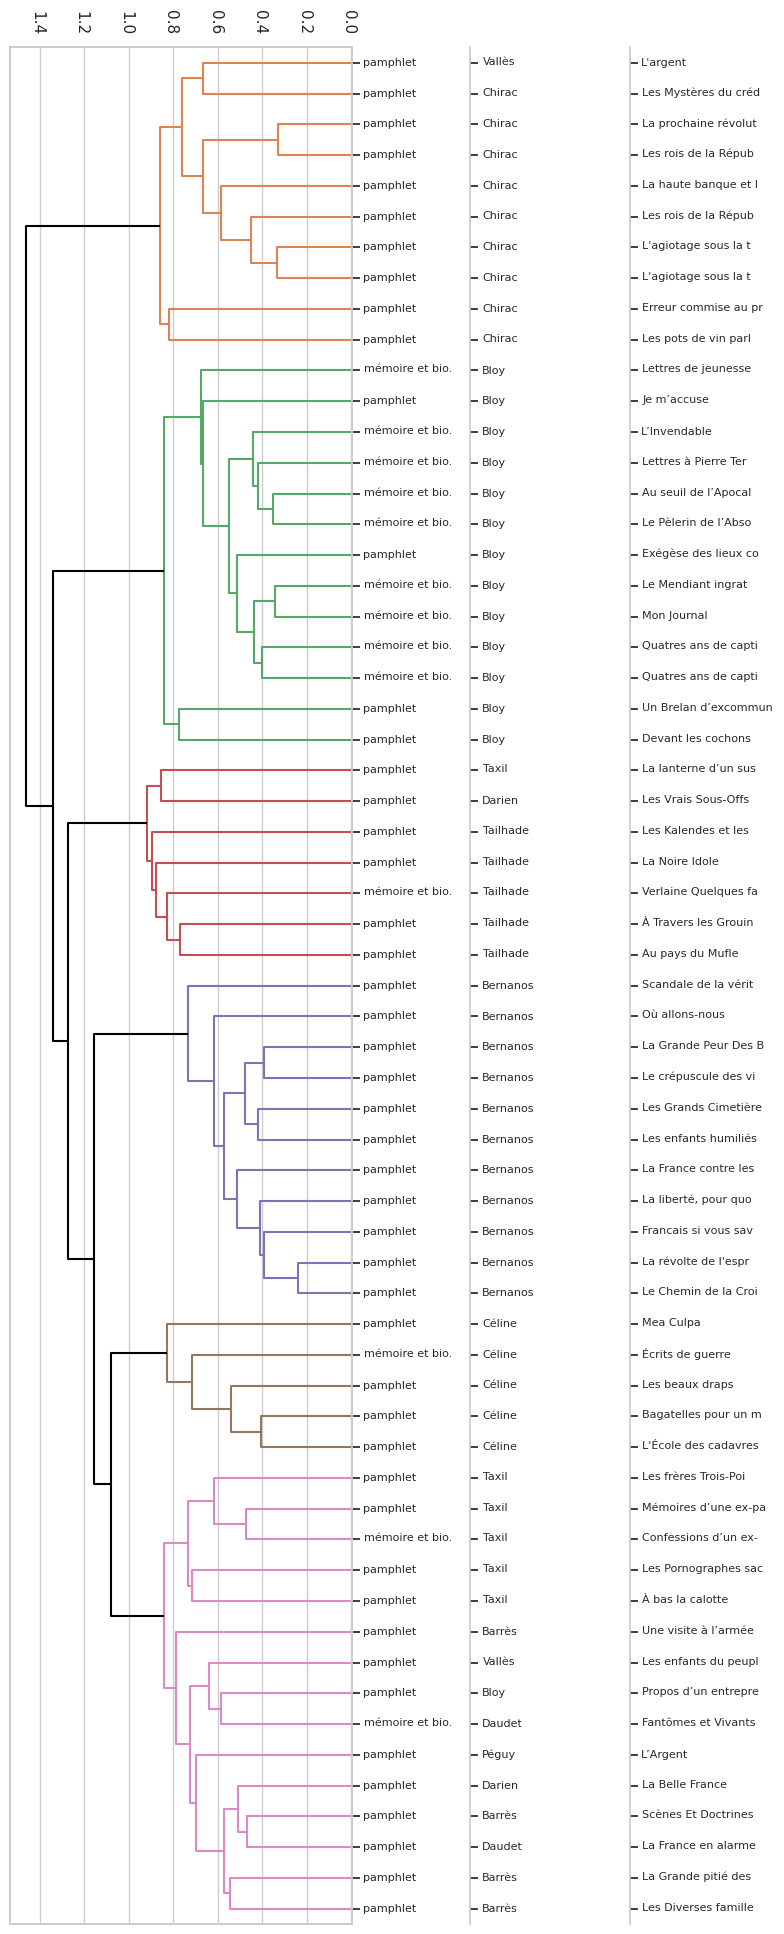
\includegraphics[width=0.60\textwidth]{img/dendogram-corpus-2-PamMem.png }
\caption{Dendrogramme de classification ascendante hiérarchique, Corpus 2, Genres pamphlet-mémoire et biographie, 1 ngram de mot, 12077 / 102851 features, 25 non nulle}
\label{'fig:dendogram-corpus-2-PamMem'}
\end{figure}

\begin{figure}[H]
\centering %
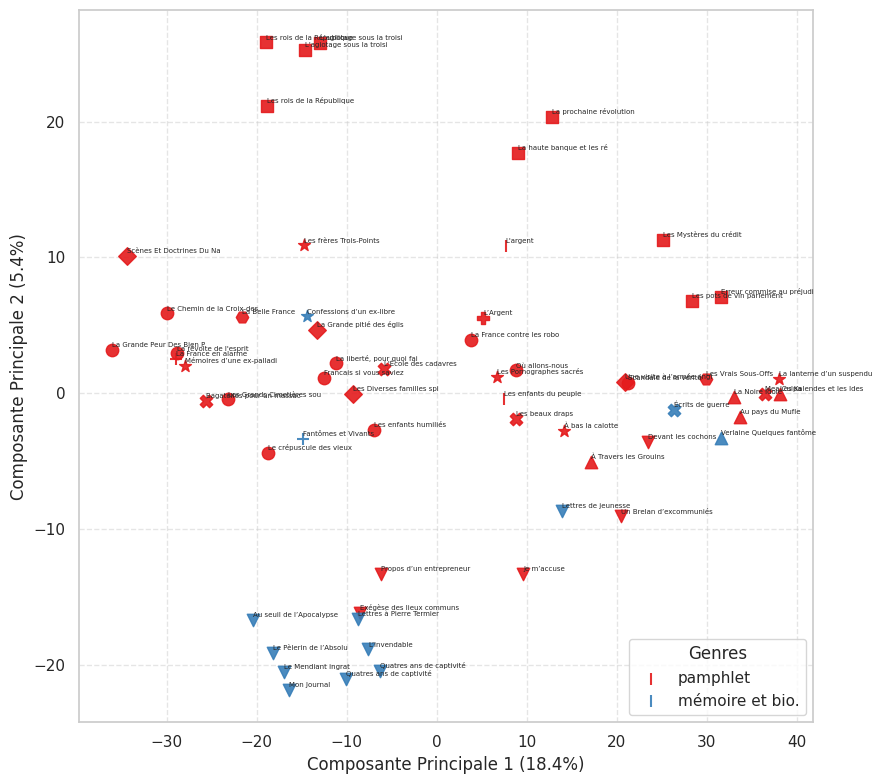
\includegraphics[width=1\textwidth]{img/ACP-corpus-2-PamMem.png}
\caption{Analyse en composantes principales, Corpus 2, Genres pamphlet-mémoire et biographie}
\label{'fig:ACP-corpus-2-PamMem'}
\end{figure}

\begin{figure}[H]
\centering %
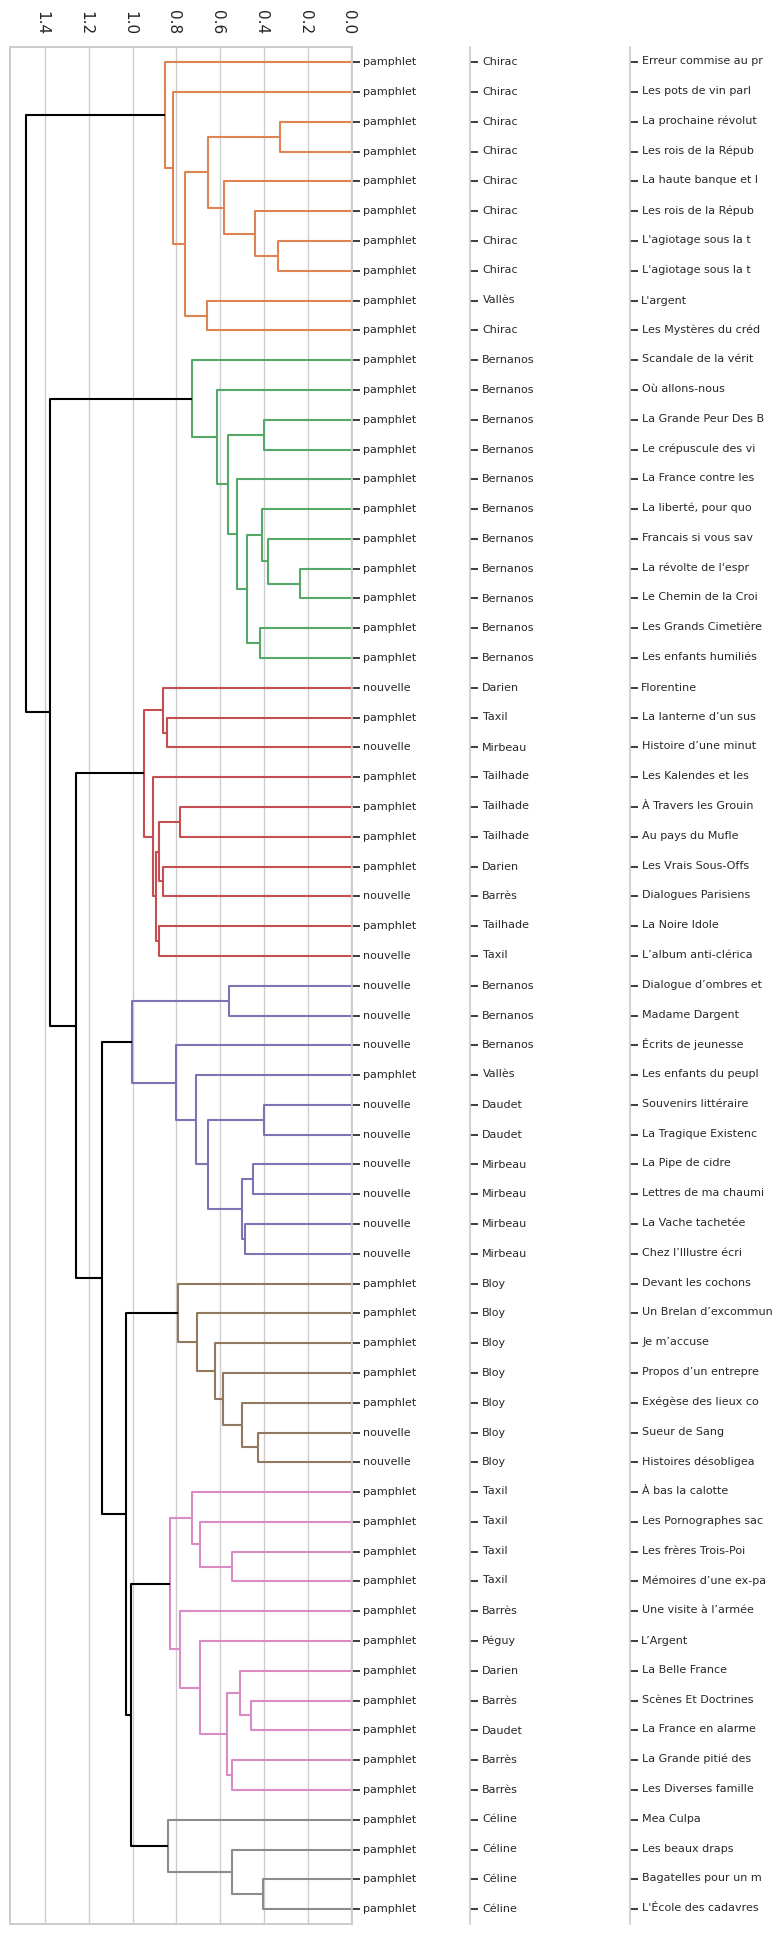
\includegraphics[width=0.60\textwidth]{img/dendogram-corpus-2-PamNouvelle.png}
\caption{Dendrogramme de classification ascendante hiérarchique, Corpus 2, Genres pamphlet-nouvelle, 1 ngram de mot, 11814 / 93079 features, 40 non nulle}
\label{'fig:dendogram-corpus-2-PamNouvelle'}
\end{figure}


\begin{figure}[H]
\centering %
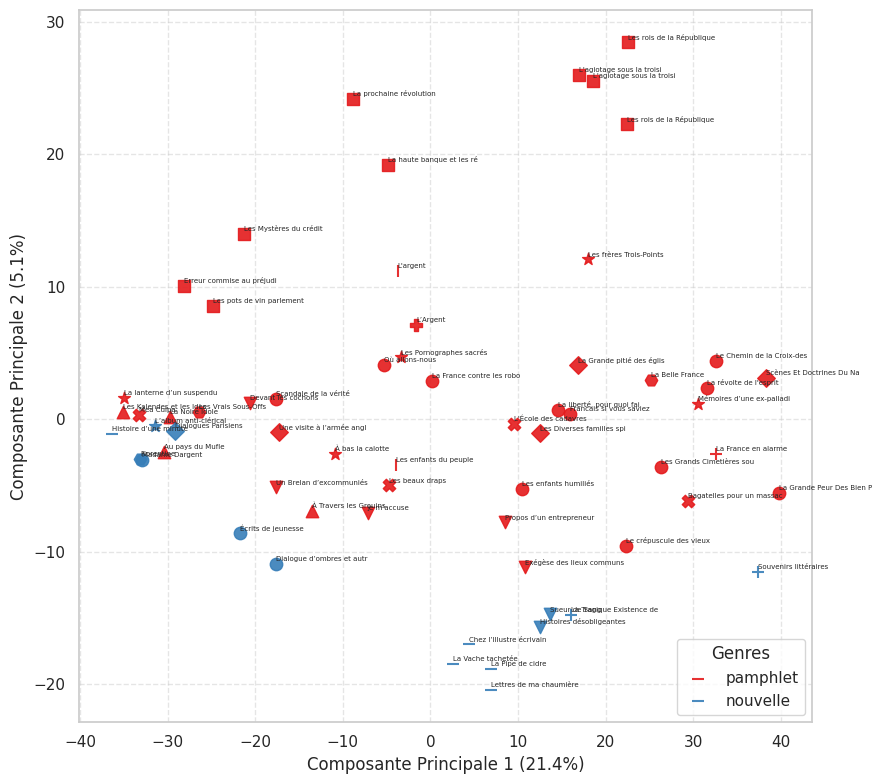
\includegraphics[width=1\textwidth]{img/ACP-corpus-2-PamNouvelle.png}
\caption{Analyse en composantes principales, Corpus 2 Genres pamphlet-nouvelle}
\label{'fig:ACP-corpus-2-PamNouvelle'}
\end{figure}
\backmatter

\listoffigures

\listoftables

\addcontentsline{toc}{chapter}{Table des matières}
\tableofcontents

\end{document}